\documentclass{aa}



% \usepackage[draft]{graphicx}
% \usepackage{txfonts}
\usepackage{amsmath}


\title{Palomar 5 Gaps}

\subtitle{Globular clusters as hole punchers}

\author{S. Ferrone
       \inst{1,2}
       \and
       P. Di Matteo\inst{2}
       \and
       M. Montuori\inst{1}
       }

\institute{Dipartimento di Fisica, Universit\`a di Roma ``La Sapienza'',
           Piazza Aldo Moro\\
           \email{salvatore.ferrone@uniroma1.it}
      \and
          Paris Observatory. Paris Sciences et Lettres\\
          \email{c.ptolemy@hipparch.uheaven.space}
          \thanks{The university of heaven temporarily does not
                  accept e-mails}
          }

\date{Born in 1996; Accepted in 2018}



\begin{document}




\abstract
  {Holy moly artichokey}
 % aims heading (mandatory)
  {ok}
 % methods heading (mandatory)
  {good}
 % results heading (mandatory)
  {alright}
 % conclusions heading (optional), leave it empty if necessary
  {done}


\maketitle
\section{Introduction}

  The presence of dark matter has substantial observational evidence on scales larger than individual galaxies. The aim of this work is to add more context to aid in the search for evidence of dark matter on the sub-galactic scale and within the Milky Way. Initially proposed by [Author Name] in [Year], the concept of dark matter emerged to explain the anomalously high velocities of stars in distant dwarf galaxies. These velocities exceed what would be expected given the visible mass exerting gravitational forces on them. Furthermore, dark matter's influence extends to cosmological scales, as evidenced by the bending of light trajectories within cosmic web filaments due to the mass of dark matter. Despite significant advancements, understanding the true nature of dark matter remains elusive, with the scientific community continually seeking evidence of its existence beyond its gravitational effects on cosmic and extragalactic scales. A current focus is the detection of dark matter at sub-galactic scales, such as through the study of stellar streams.

  Stellar streams, which are long, thin structures formed from the tidal disruption of globular clusters or dwarf galaxies as they orbit a host galaxy, offer a promising avenue for probing the distribution of dark matter. Tidal forces arise because these stellar systems are extended objects, leading to a differential gravitational pull across their structure. As a result, stars farther from the galactic center lag behind the cluster, while those closer are pulled away. This process stretches the cluster in the radial direction, creating two tidal tails that trace the orbit of the cluster. Theoretical predictions of this phenomenon have long existed, but it was not until the early 1995 that streams were observed for the first time \citet{carl_j_grillmair_globular_1995}. Then, \citet{odenkirchen_detection_2001} discovered that stars beyond the tidal radius of the Palomar 5 cluster shared the same spectroscopic characteristics as those within it.

  Over the past two decades, both theoretical and numerical studies have demonstrated the utility of stellar streams in constraining the gravitational field of host galaxies, particularly the Milky Way. Galactic dynamics, governed by Poisson's equation, allow the decomposition of a galaxy into components such as the central bulge, disk, and dark matter halo. The dark matter halo, often modeled as spherical, is the largest component and plays a critical role in the observed constant rotational velocity of galaxies. However, determining whether the halo might be an oblate spheroid could provide insight into the self-interaction properties of dark matter. Numerical studies, such as those by \citet{varghese2011stellar} who explored the extent to which stellar streams can constrain the galactic potential under varying levels of observational data. Meanwhile, Bonaca et al. approached stellar streams from an information-theoretic perspective, identifying the orbits and configurations that yield the most information about the galactic potential.

  The release of Gaia Data Release 2 (DR2) and DR3 significantly advanced the observational study of stellar streams. The StreamFinder algorithm has identified 90 stellar streams, with some of these candidates being followed up by other instruments and surveys. For instance, streams like GD-1 and Palomar 5 have approximately 1,000 to 3,000 currently associated members, although there is an observational bias toward brighter stars, such as red giants.

  The goal of this study is to contribute to the ongoing effort to use stellar streams as probes for dark matter on sub-galactic scales. According to the cold dark matter model, which is supported by observations, galaxies form hierarchically, leading to a mass distribution of dark matter subhalos that follows a power-law. This suggests that numerous small dark matter clumps should exist within galaxies. \citet{rodrigo_ibata_uncovering_2002} suggested that the presence of said dark matter subhaloes dark matter subhalos can influence the stellar streams by diffussing their distribution of orbital elements. \citet{r_g_carlberg_pal_2012} extended this idea by noting that subhaloes could have flybys and that leave gaps in stellar streams and subsquently explored the statistical distribution the number of gaps gaps given a probabilistic model of the rate of encounters given based on the expected distribution of dark matter subhalos. \citet{bonaca_spur_2018} took a more direct observational approach, identifying an underdensity in the GD-1 stream that could not be explained by known objects like globular clusters and was inconsistent with the mass-size relationship predicted by the Lambda-CDM model.

  In this study, we aim to investigate the potential influence of globular clusters on stellar streams, specifically examining whether galactic globular clusters can produce gaps similar to those expected from dark matter subhalos. If globular clusters do create significant gaps, this must be considered when using stellar streams to infer the local presence of dark matter. Our focus is on the Palomar 5 stream, which has been well-studied and has observable gaps, a high membership count, and favorable visibility due to its position above the galactic disk. In the following sections, we describe the modeling of this stream, the gravitational interactions with the galaxy and other globular clusters, and the statistical analysis of the perturbations affecting the stream.













\section{Methods}



  \subsection{Numerical Methodology}
    Our numerical methodology follows the approach outlined in Ferrone et al. (2023), which we briefly summarize here for completeness. We begin by extracting the phase space properties (positions, velocities) as well as the masses and half-mass radii of 165 globular clusters from the dataset provided by Baumgardt and Vasiliev et al. The dataset includes the clusters' masses, radial velocities, distances, proper motions in RA and DEC, and their associated covariance terms.

    To generate initial conditions, we treat the five-dimensional phase space variables (position and velocity components) for each globular cluster as Gaussian distributions. Using the \texttt{np.random.gauss} function, we generate 50 samples per cluster, producing 50 sets of initial conditions for the entire globular cluster system. These samples are stored in data files for later use.

    Next, we convert the initial conditions into a galactocentric reference frame. The local standard of rest was computed using XXX, with the Sun's peculiar velocity set to XXX, and the Sun's distance from the Galactic center taken as XXX. These transformations were performed using the \texttt{astropy} package.

    For the galactic potential, we employed the static model proposed by Pouliasis et al. (2017), which consists of a superposition of a thin disk, thick disk, and a dark matter halo. This model is assumed to be time-independent over the course of our simulations.

    The primary methodological departure from Ferrone et al. (2023) is that now we include globular cluster interactions. Instead of treating the clusters as point masses that only experience the gravitational potential of the galaxy, we now compute N-body interactions between the clusters during the backward integration over 5 billion years. Although these interactions were included, we observed no significant exchanges of orbital energy or momentum between clusters. The resulting orbits were saved to data files for subsequent analysis.

    At the computed positions 5 Gyr ago, each globular cluster was replaced by a system of 100,000 particles, sampled from a Plummer distribution to represent the stellar content of the cluster. We then integrated the evolution of these particles forward in time to the present day. During this forward integration, each star particle feels the gravitational influence of the galaxy and all globular clusters, but not other star particles. We do not perform direct N-body simulations between star particles; instead, at each time step, we compute the positions of all globular clusters and apply their forces to the star particles.

    The integration was performed using a leapfrog integrator. The timestep was chosen to be sufficiently small to ensure both the conservation of energy and that the integration error over 5 Gyr was negligible compared to the scale radius of the globular clusters. Further details on the timestep selection are discussed in the appendix.

    During the integration, intermediate snapshots were saved to facilitate the analysis of stellar streams and the effects of cluster impacts. Specifically, for each of the 50 realizations of the Palomar 5 stream, we saved 5,000 intermediate timesteps, resulting in approximately XX GB of data ($N_p \times N_s \times 7 \times \text{float}$).




  \subsection{Gap detection}

    At the end of the simulations, some gaps in the stellar stream are so prominent that they can be identified visually without any sophisticated quantitative analysis. However, upon closer inspection, more subtle gaps emerge, highlighting the need for quantitative methods to systematically detect and assess these features.

    We initially sought an automated, quantitative approach from signal and image processing that could reliably detect all gaps and evaluate their significance. Unfortunately, despite extensive efforts, an ideal method remained elusive. As a result, we opted for a simpler approach: a combination of visual inspection aided by comparative analysis.

    To facilitate this process, we ran a series of \texttt{vanilla} simulations. In these control simulations, we used the same 50 sets of initial conditions but excluded interactions between globular clusters and omitted the gravitational influence of the clusters on the star particles within the stream. By comparing the morphological differences between these control simulations and the full simulations (which included cluster interactions), we could identify and assess the impact of globular clusters on the stream structure more effectively.


    Comparisons between the \texttt{vanilla} and full simulations  were performed in the tail coordinate system. This system allows for consistent morphological comparisons by aligning the stream with the cluster's orbit. The coordinate system is based on the work of Dehnen et al. (2004) and is detailed in Appendix~\ref{appendix:TailCoordinates}.

    Briefly, the x'coordinate represents the position of a particle along the orbit relative to the globular cluster—whether it is ahead or behind the cluster. The y' coordinate measures the particle's distance within the orbital plane, where positive values indicate that the particle is farther from the Galactic center and negative values indicate that it is closer.

    \subsubsection*{Density maps and profiles}
      For each of the 50 simulations, we compare the final snapshots between the \texttt{vanilla} and full simulations in the tail coordinate system. We inspect these differences by creating 2D density maps of the streams. Subsequently, we wish to employ a quantitative method to make detections discover when the \textit{full} simulations are significantly less dense than the \textit{vanilla} simulations. To do so, we marginalize over the y'-coordinate to produce 1D density profiles along the x'-axis. These comparisons are illustrated in the results section (see Fig.~\ref{fig:profiles}).

      To construct the 1D density profiles, we first bin the data using the $\sqrt{N}$-rule for determining the number of bins, where N is the number of data points which is 10$^5$. After histogramming the 1D profiles, we apply a boxcar smoothing technique, where each central value is replaced by the median of the surrounding XX adjacent data points, corresponding to a smoothing length of approximately 300 parsecs. This procedure reduces high-frequency noise and smooths the profiles, as shown in Fig.~\ref{fig:profiles}, where the center of mass has been effectively removed.


      With the smoothed 1D density profiles in hand, we consider the \textit{vanilla} simulations to be truth, and search for locations that are significantly less dense than \textit{vanilla} in a way that is greater than stochastic chance. To do so, we first compute the log ratio of the two profiles:
      \begin{equation}
        \mathcal{R} = \log\left(\frac{\rho_f}{\rho_v}\right),
        \end{equation}
      where $\rho$ is the 1D density, $v$ corresponding to the vanilla simulation, and $f$ corresponding to the full simulation, and $R$ is the log ratio of the two. Using the log ratio is important, because the distribution is symmetric and zero centered. For example if we only used the ratio, then the codomain would be $\frac{\rho_f}{\rho_v} \in [1,+\inf]$ for $\rho_f > \rho_v$, and $\frac{\rho_f}{\rho_v} \in [0,1]$ for $\rho_f < \rho_v$. 

      Yet, we only wish to consider bins with a significant amount of counts. We find this threshold by asserting that the signal to noise ratio must be greater than 50. The signal is based on the \textit{vanilla} profile, and the noise is the error propogation given poisson uncertainties for the number of counts a given bin: 
      \begin{equation}
        \mathcal{S}/\mathcal{N} =50= \frac{\log{N}}{\frac{1}{\ln(10)} \sqrt{N}}
        \end{equation}



      

      
      we compute the difference between the logarithms of the binned counts for each profile and search for points that fall more than two standard deviations below the mean. However, we only consider regions that surpass a predefined significance threshold, where the significance is determined by the uncertainties in the binned counts governed by Poisson statistics multiplied by a factor of 50. This noise floor was chosen to eliminate the low-density regions near Palomar 5, where gaps are more likely caused by epicyclic oscillations rather than impacts from globular clusters. The identified gap candidates are marked and labeled on the plots.

      This method, however, is not without limitations, particularly when detecting smaller gaps. As discussed in Erkal et al. (2015), a gap's size is not necessarily indicative of a weak impact but could result from a more recent interaction. Additionally, because our streams have finite width, some gaps may be oriented obliquely relative to the stream axis. In these cases, marginalizing over y' can dilute the gap's signal, making it difficult to detect. An example of this is the small gap around 5 kpc, which, as we will demonstrate later, is caused by the interaction with NGC 2808 and appears in most simulations. 


    \subsubsection*{From Suspect to Culprit} \label{SuspectToCulprit}

      A key question we seek to answer is: from the gaps present at the end of the simulation, who caused them? To address this, we examine the evolution of stream density over time. Instead of using the x'coordinate, we introduce $\tau$, which represents time rather than distance. Specifically, $\tau$ indicates how long it will take for a cluster to reach, or how long ago it passed, a given point on its orbit. This is advantageous because the growth of the stream is approximately linear in $\tau$ whereas in physical space, streams on eccentric orbits expand and contract depending on the orbital phase.


      \citet{sanders2016dynamics} extended the analysis of Erkal et al. (2015), demonstrating that action-angle variables provide a useful coordinate system for analyzing stream evolution, as actions are conserved and the angles associated with the stream's growth evolve linearly over time. Although we became aware of this work only after completing our analysis, we note that $\tau$ is a suitable approximation and behaves similarly to the angle variable corresponding to the azimuthal action: $\tau \approx \theta_{\phi,i} - \theta_{\phi,\text{GC}}$

      The core of our analysis is presented in Fig.~XXX. The bottom panel shows the evolution of the stream density over time. To avoid extreme low-density regions at the stream's edges, we applied a density threshold to focus on the more significant areas of the stream. Next, we modeled Palomar 5's orbit as a proxy for its stream and sampled points along the orbit to measure the gravitational force exerted by other globular clusters. This force data is displayed in the top panel of Fig.~XXX, showing how the total gravitational acceleration on Palomar 5's stream evolves over its length throughout the simulation.

      We then used \texttt{scipy}'s \texttt{ndimage} package to identify the top five local maxima in the data space of gravitational acceleration $\vec{g}$ as a function of time $t$ and the stream coordinate $\tau$. Once these local maxima were identified, we iterated over the contributions of individual globular clusters to determine which cluster contributed the most to each peak in $\vec{g}$. Each significant peak was labeled with the corresponding globular cluster.


      Afterward, we cross-referenced these peaks with the previously identified gaps in the stream. For large gaps resulting from strong interactions, we observed that after an impact, a low-density wake is left behind in the ($t,\tau$) plane.

      The results of this analysis were compiled into a table. If a gap was attributed to a particular globular cluster, it was labeled as \texttt{TRUE}; otherwise, it was marked as \texttt{FALSE}. For a handful of simulations, to double check that the verdict made correctly when passing from suspect to culprit, we re-compute the simulations yet individually adding one globular cluster at a time. As a result, we are able to confirm that singular gaps arrise from the suspected clusters.  


  \subsection{Reconstruction of the impact geometry}
    In its simplest form, impact theory, as presented in works such as Binney and Tremaine, John Taylor, and Galaxies, considers two particles: one stationary and the other moving past it. The distance between the two particles at their closest approach is known as the impact parameter. To simplify the analysis, the \textit{impulse approximation} is often employed, which assumes that the velocity of the perturber remains unchanged during the interaction. This assumption greatly simplifies the computation.

    To understand how the impacted particle is perturbed, one needs to compute its change in momentum, which is determined by integrating the force acting on the particle over the duration of the interaction. A useful approximation for this change in momentum is the force at the closest approach multiplied by an estimate of the interaction time:
    \begin{equation} 
      \Delta p \approx \text{Force} \times \text{interaction time} = \frac{GMm}{b^2} \times \frac{b}{v} = \frac{GM}{bv}, 
      \end{equation}
    where $M$ is the mass of the perturber, $m$ is the mass of the particle, $b$ is the impact parameter, $v$ is the relative velocity of the perturber with respect to the particle, and $G$ is the gravitational constant.

    From this analysis, we can conclude that a more massive perturber, passing closer to the particle, and moving more slowly, will have a greater impact. It's important to note that the momentum change is inversely proportional to the velocity of the perturber, which contrasts with the intuition from elastic collisions, such as those between billiard balls, where higher velocities generally result in greater impact.

    Erkal et al. (2015) extended this impact theory to a one-dimensional stream, studying how the momentum change of a particle varies as a function of its distance from the point of impact. In their analysis, the perturber was modeled not as a point mass, but as a Plummer sphere with a characteristic length scale $r_p$. Since the stream is not zero-dimensional and has length, both the parallel and perpendicular components of the velocity must be considered. Consequently, five parameters determine the change in velocity of a given particle: $M$, $r_p$, $b$, $W_\parallel$, and $W_\perp$. Our goal is to constrain these parameters during the impact in our simulations and compare them to close approaches that do not generate gaps, in order to establish the criteria necessary for gap formation.

    To achieve this, we begin by identifying the approximate moments of impact from the most significant clusters, as determined in the previous analysis in Sec.~\ref{SuspectToCulprit}. Then, we refine these estimates. While the orbit serves as a good first-order proxy for the stream, it is insufficient, as the typical offset between the stream and its orbit can be on the order of 200-400 pc—significantly larger than the impact parameters we are investigating.

    In this refinement process, we aim to pinpoint both the exact location of the impact along the stream and the precise moment it occurred. To do so, we fit a third-order parametric polynomial to the stream, using the saved snapshots from our simulations.
    \begin{align}
      x(\tau) &= a_0 + a_1 \tau + a_2 \tau^2 + a_3 \tau^3, \\ 
      y(\tau) &= b_0 + b_1 \tau + b_2 \tau^2 + b_3 \tau^3, \\
      z(\tau) &= c_0 + c_1 \tau + c_2 \tau^2 + c_3 \tau^3,
      \end{align}
    where $x$, $y$, and $z$ represent the parametric line describing the stream in galactocentric coordinates, $\tau$ is the stream coordinate in time as described in the previous section, and is used as the independent variable in this analysis. The coefficients $a_i$, $b_i$, and $c_i$ are the polynomial coefficients. We found that a second-order polynomial was insufficient to capture the curvature along the full length of the stream, with divergence from the star particle positions occurring at the extremes. A third-order polynomial was sufficient and desirable, as it is the lowest order that adequately captures the path of the stream over the entire length under consideration.

    In this analysis, only one side of the stream is considered. For instance, if the impact candidate was in the leading tail, only the star particles with $\tau > 0$ are used to constrain the stream. The polynomial coefficients were determined using the Nelder-Mead algorithm from \texttt{scipy}'s optimization package.

    Since the simulation snapshots were saved at a temporal resolution of 1 Myr—rather than at the integration timestep of $10^4$ years, which would generate an excessive amount of data—we interpolate between snapshots to more precisely estimate the impact geometry. This is achieved by fitting the stream at five timesteps surrounding the approximate impact time, a period of 5 Myr, which sufficiently covers the interaction time. The interaction time can be estimated as $t \approx \frac{100~\text{pc}}{300~\frac{\text{km}}{\text{s}}} \approx 0.3~\text{Myr}$.

    As a result, each polynomial coefficient can now be expressed as a function of time. Consequently, we can parameterize the stream as a function of both simulation time and position along the stream:

    \begin{align}
      x(t,\tau) &= a_0(t) + a_1(t)\tau + a_2(t) \tau^2 + a_3(t)\tau^3, \\ 
      y(t,\tau) &= b_0(t) + b_1(t)\tau + b_2(t) \tau^2 + b_3(t)\tau^3, \\
      z(t,\tau) &= c_0(t) + c_1(t)\tau + c_2(t) \tau^2 + c_3(t)\tau^3.
      \end{align}
    The values of the coefficients as a function of time are obtained through linear interpolation, ensuring that the coefficients at the snapshot times match the values constrained by the simulation data.

    Next, we fit the trajectory of the perturber with a second-order polynomial. With equations for both the stream and the perturber as functions of time, we identify the time and location of impact by minimizing a cost function, defined as the distance between the stream and the perturber:

    \begin{equation} b(t, \tau) = \left\lVert \vec{s}(t, \tau) - \vec{p}(t) \right\rVert, \end{equation}

    where $\vec{s}(t, \tau)$ is the galactocentric position of a point on the stream, $\vec{p}(t)$ is the position of the perturber, and $b$ is the distance between the two. The minimum value of $b$, denoted as $\text{min}(b)$, represents the impact parameter. The minimization is carried out using \texttt{scipy}'s optimization package with the \textit{L-BFGS-B} method, which allows us to constrain $t$ and $\tau$, ensuring no extrapolation occurs.

    Once this minimization is performed, determining the relative velocity becomes straightforward. Since the minimization provides the impact parameter, time of impact, and corresponding value of $\tau$, we can compute the derivatives of the parametric equations at $t_{\text{min}}$ and $\tau_{\text{min}}$. The parallel and perpendicular components of the perturber's velocity relative to the stream are given by:

    \begin{align}
      \Delta \vec{v} &=\vec{v_p} - \vec{v_s} \\
      w_\parallel &= \left(\Delta \vec{v}\right)\cdot \hat{v_s}\\  
      w_\perp &=  \sqrt{\Delta v ^2 - w_\parallel ^ 2}
      \end{align}


    where $\vec{v}_p$ and $\vec{v}_s$ are the velocities of the perturber and the stream, respectively. For each of the 50 simulations, this information was compute for the strongs 5 flybys of a perturber with the stream. Thus, we compute a sample of 250 impacts, and flag those that give way to gaps. 


\section{Results}

  I'm gonna go remake the figures before I adapt the text. However, before that, I will say the general outline of the flow of the article. I will show a general result here, which is what we would expect to see on the sky, which is comparable with reality. It's a great first figure becuase it shows the essence of the paper. Then, I pretty much follow the methodology and keep the story the same with just monte-carlo-009. The story is we need to understand how many gaps are present in a given simulation, then we need to identidy who the perturbers are. So step 1 (fig 2) shows our aided eye-test. Fig~3 shows how I tried to find each perturber, and Fig~4 shows a sanity check to reassure me that the suspects are indeed guilty. However, I will say that we picked monte-carlo-009 because it has two obvious gaps and two subtle ones, which aid in communicating our point. A full display of the gaps in our simulations is shown in the appendix (i'll make pair-plots with vanilla and full simulations above and below one another with the gaps labeled. :D ) 

  After we discuss the magic to make detections, I THEN will discuss some general properties, i.e. is there something special about these perturbers compared to other clusters? The main results is that \textit{you need to enter Pal5's orbital space}, which is not a shocker. If you can hit me, you can't perturb me. NEXT, I want to compare the population of perturbers to all globular clusters based on their internal parameters, so here we do show a tendency. Next, I wanna show how often gaps appear, and thus how many time a given GC pertubered Pal5, and when the gaps occur. I think a conclusion with the histograms in time is 

  Lastly, I will try to show something about the impact geometry. I will state that we want to compare the ones that create gaps to those that did not. We wanted to apply what we learned from Carlberg, Erkal and Sanders. The moral of the story will be that, no combination of parameters explaining the geometry cleared demarcated the presence of a gap or not. This can be inline with Sander's expanion of the analysis initiated by Carlberg and extended by Erkal. Namly, a uniformly dense stream on a circular orbit is just not good enough. I think Sanders also said that the streams needs to be sufficiently diffuse, which could make sense given the epicycles. 


  \textbf{\textit{Action item:}} I need to make sure I check out real good the papers that investigate the gaps from Palomar 5. I wanna compare this to the known length of Palomar 5, how does this reduce the results, and are there observed gaps in Palomar 5 that are consistent with these simulations? 


  \begin{figure*}
    \centering
    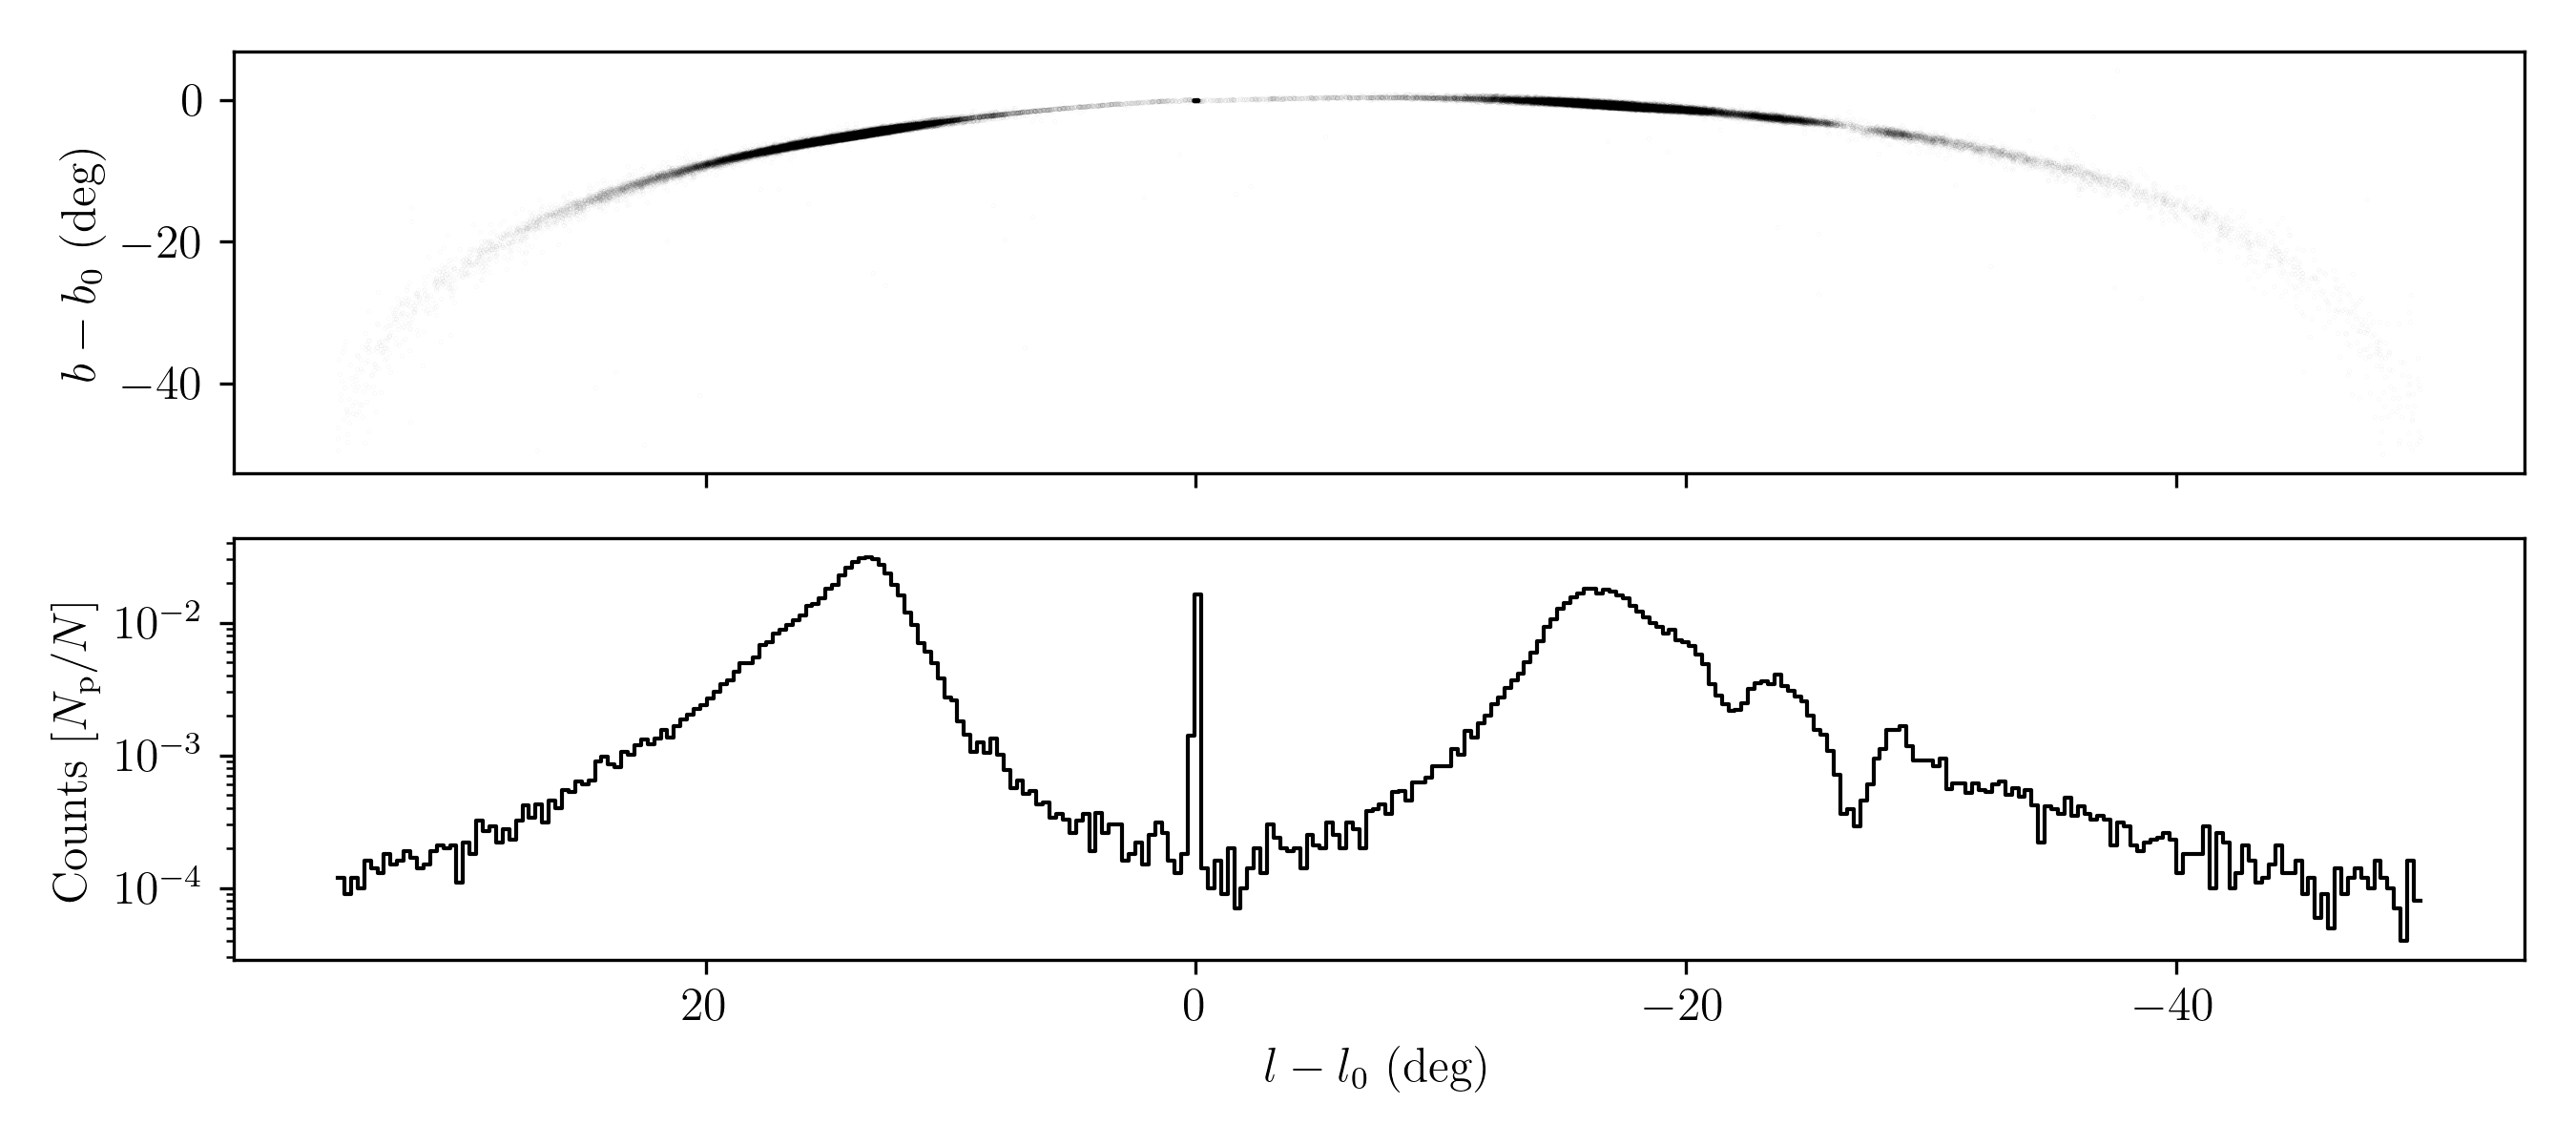
\includegraphics[width=\linewidth]{stream_on_sky_Pal5_monte-carlo-009_pouliasis2017pii-GCNBody.png}
    \caption[]{A model of the Palomar 5 stream in an axis-symmetric galactic potential plus all other globular clusters. The top plot is a scatter plot of star-particles that escaped the cluster due to tidal forces, the bottom plot shows the marginalized 1D density profile in longitude. Two large gaps are present and are due to the passage of two globular clusters. }
    \end{figure*}


  \begin{figure*}
    \centering
    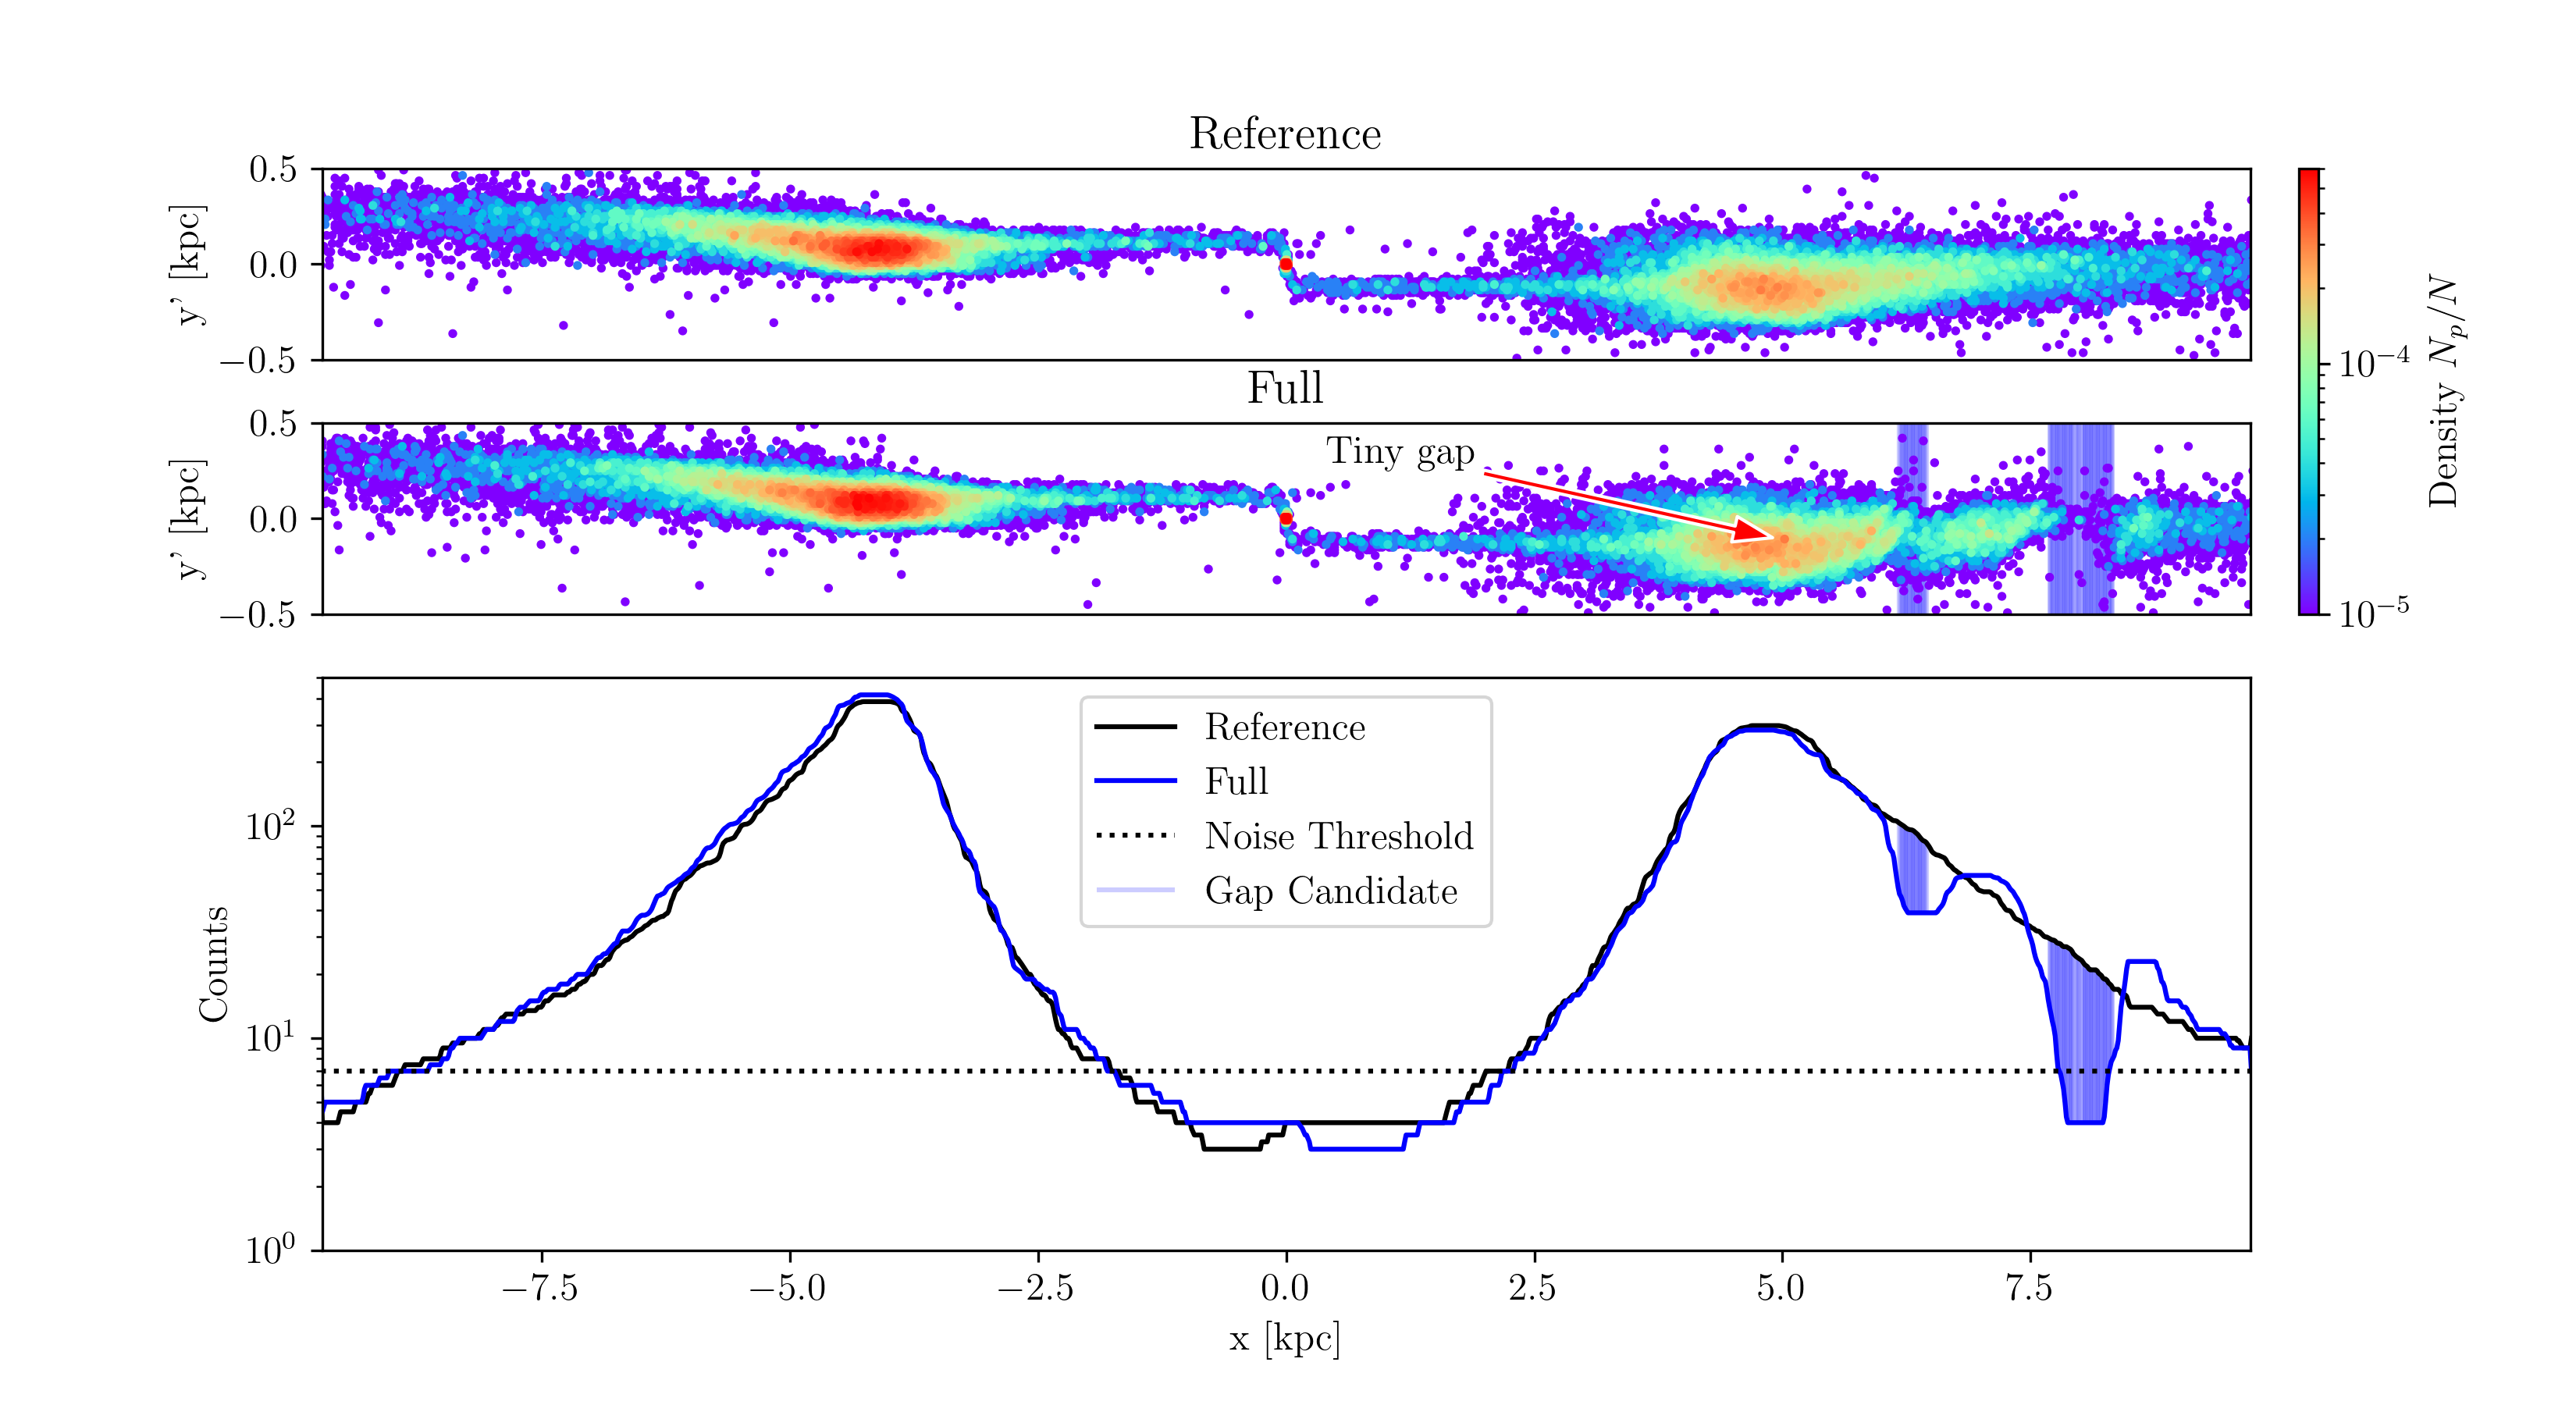
\includegraphics[width=\linewidth, trim=20 0 15 0]{monte-carlo-009-pouliasis2017pii-GCNBody-2000-milisigma-5-noisefactor-20-boxcarindexlength-shifted-0.png}
    \caption[]{A comparison between the vanilla and full simulations. This showcases our gap detection method, in which the 2D maps in \textit{tail coordinates} are inspected, and their 1D marginalized density distributions are compared quantitatively. The $x'$ coordinate indicates distance from the center of mass of Pal5 along it's orbit. The two profiles are subtraced in locations where the signal is above the noise threshold, and locations that are more that are underdense by 2-$\sigma$ are highlighted with vertical blue lines, and labeled \textit{gap candidate}. This also showcases the limitation in this 1D profile method since a very skinny and oblique gap is present, whose signal is washed out from marginalizing.}
    \label{fig:profiles}
    \end{figure*}  


  \begin{figure*}
    \centering
    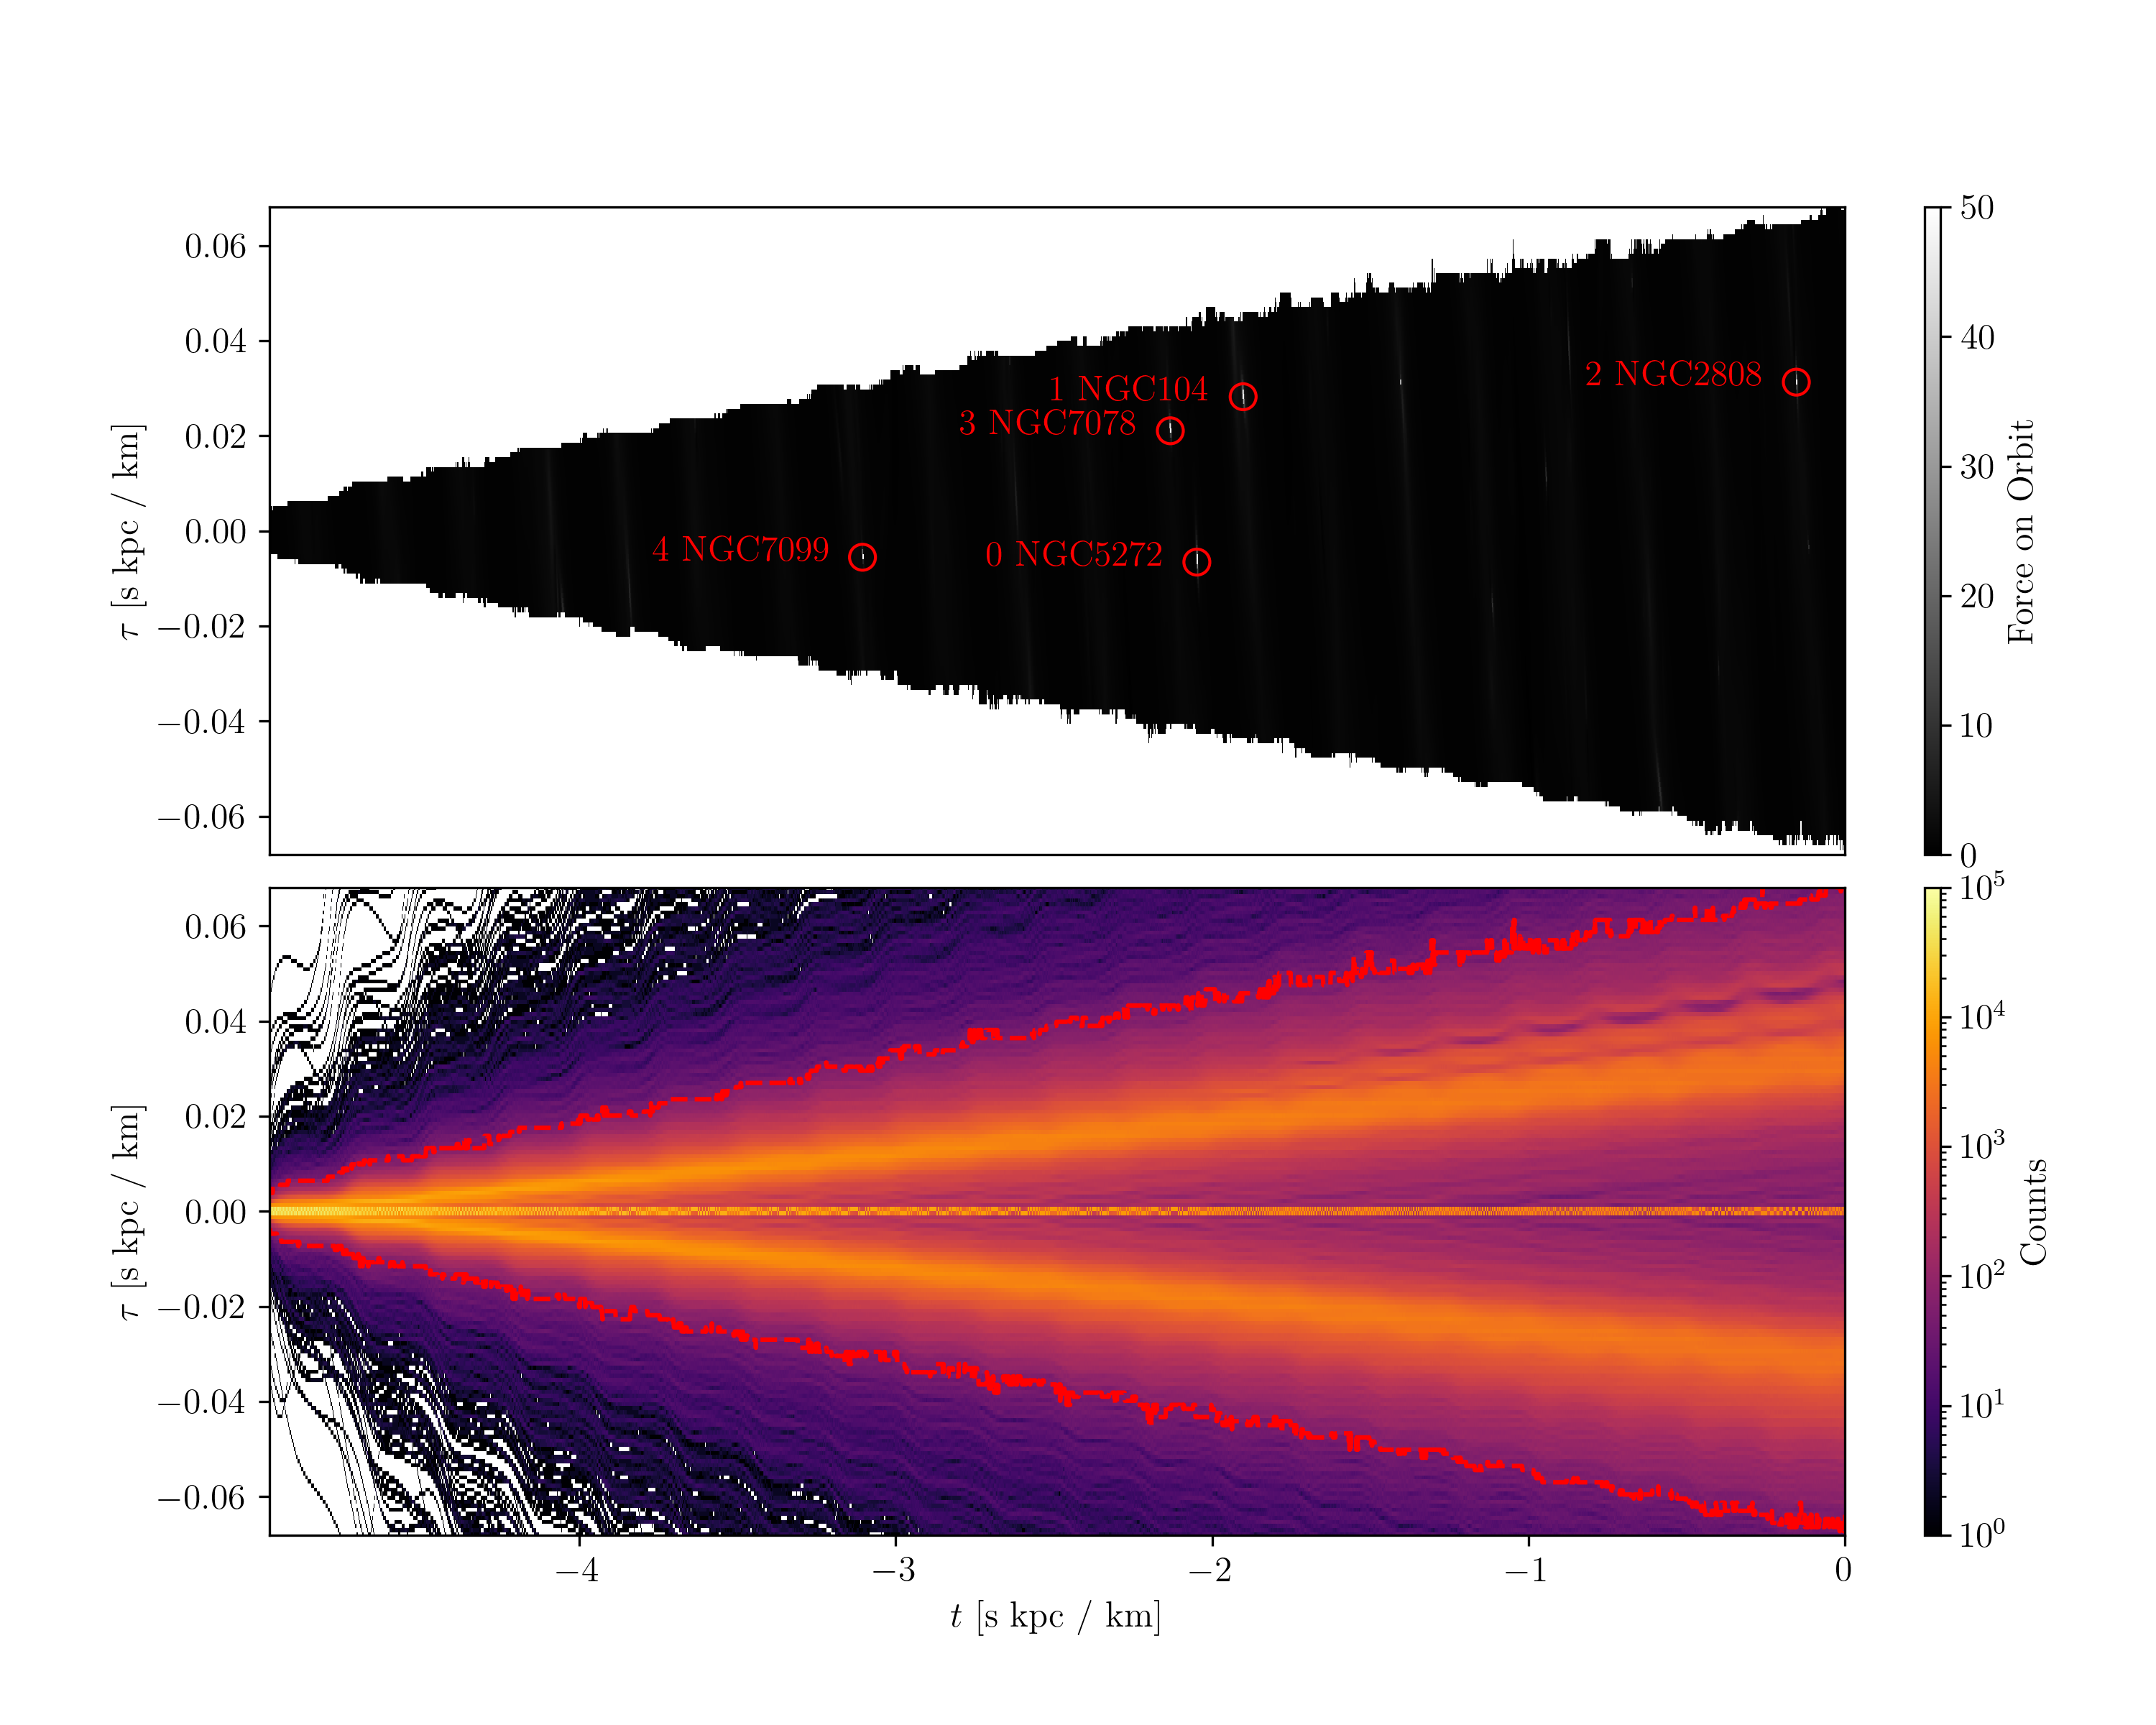
\includegraphics[width=\linewidth]{force_on_orbit-monte-carlo-009.png}
    \caption[]{This figure demonstrates how we determined which globular clusters were responsible for the gaps. The bottom plot showcases the evolution of the stream density in simulation time. The y-axis is $\tau$, which is a coordinate in units of time that indicates how far ahead or behind it is from a globular cluster. The x-axis is the simulation time, $t$, where 0~s km~kpc$^{-1}$ indicates present time. The density was used to determine a sutible length of the stream as a function of time. This length was then used to extract a piece of Palomar 5's orbit about a given position of Pal 5 in time. This orbital segment is used to approximate the stream. Then, the gravitational force from all other clusers was computed on the orbit. Moments of high acceleration indicate the passage of another cluster. The top 5 strongest passages are labeled with red circles as well as the name of the clusters. }
    \label{fig:profiles}
    \end{figure*}  



  \begin{figure*}
    \centering
    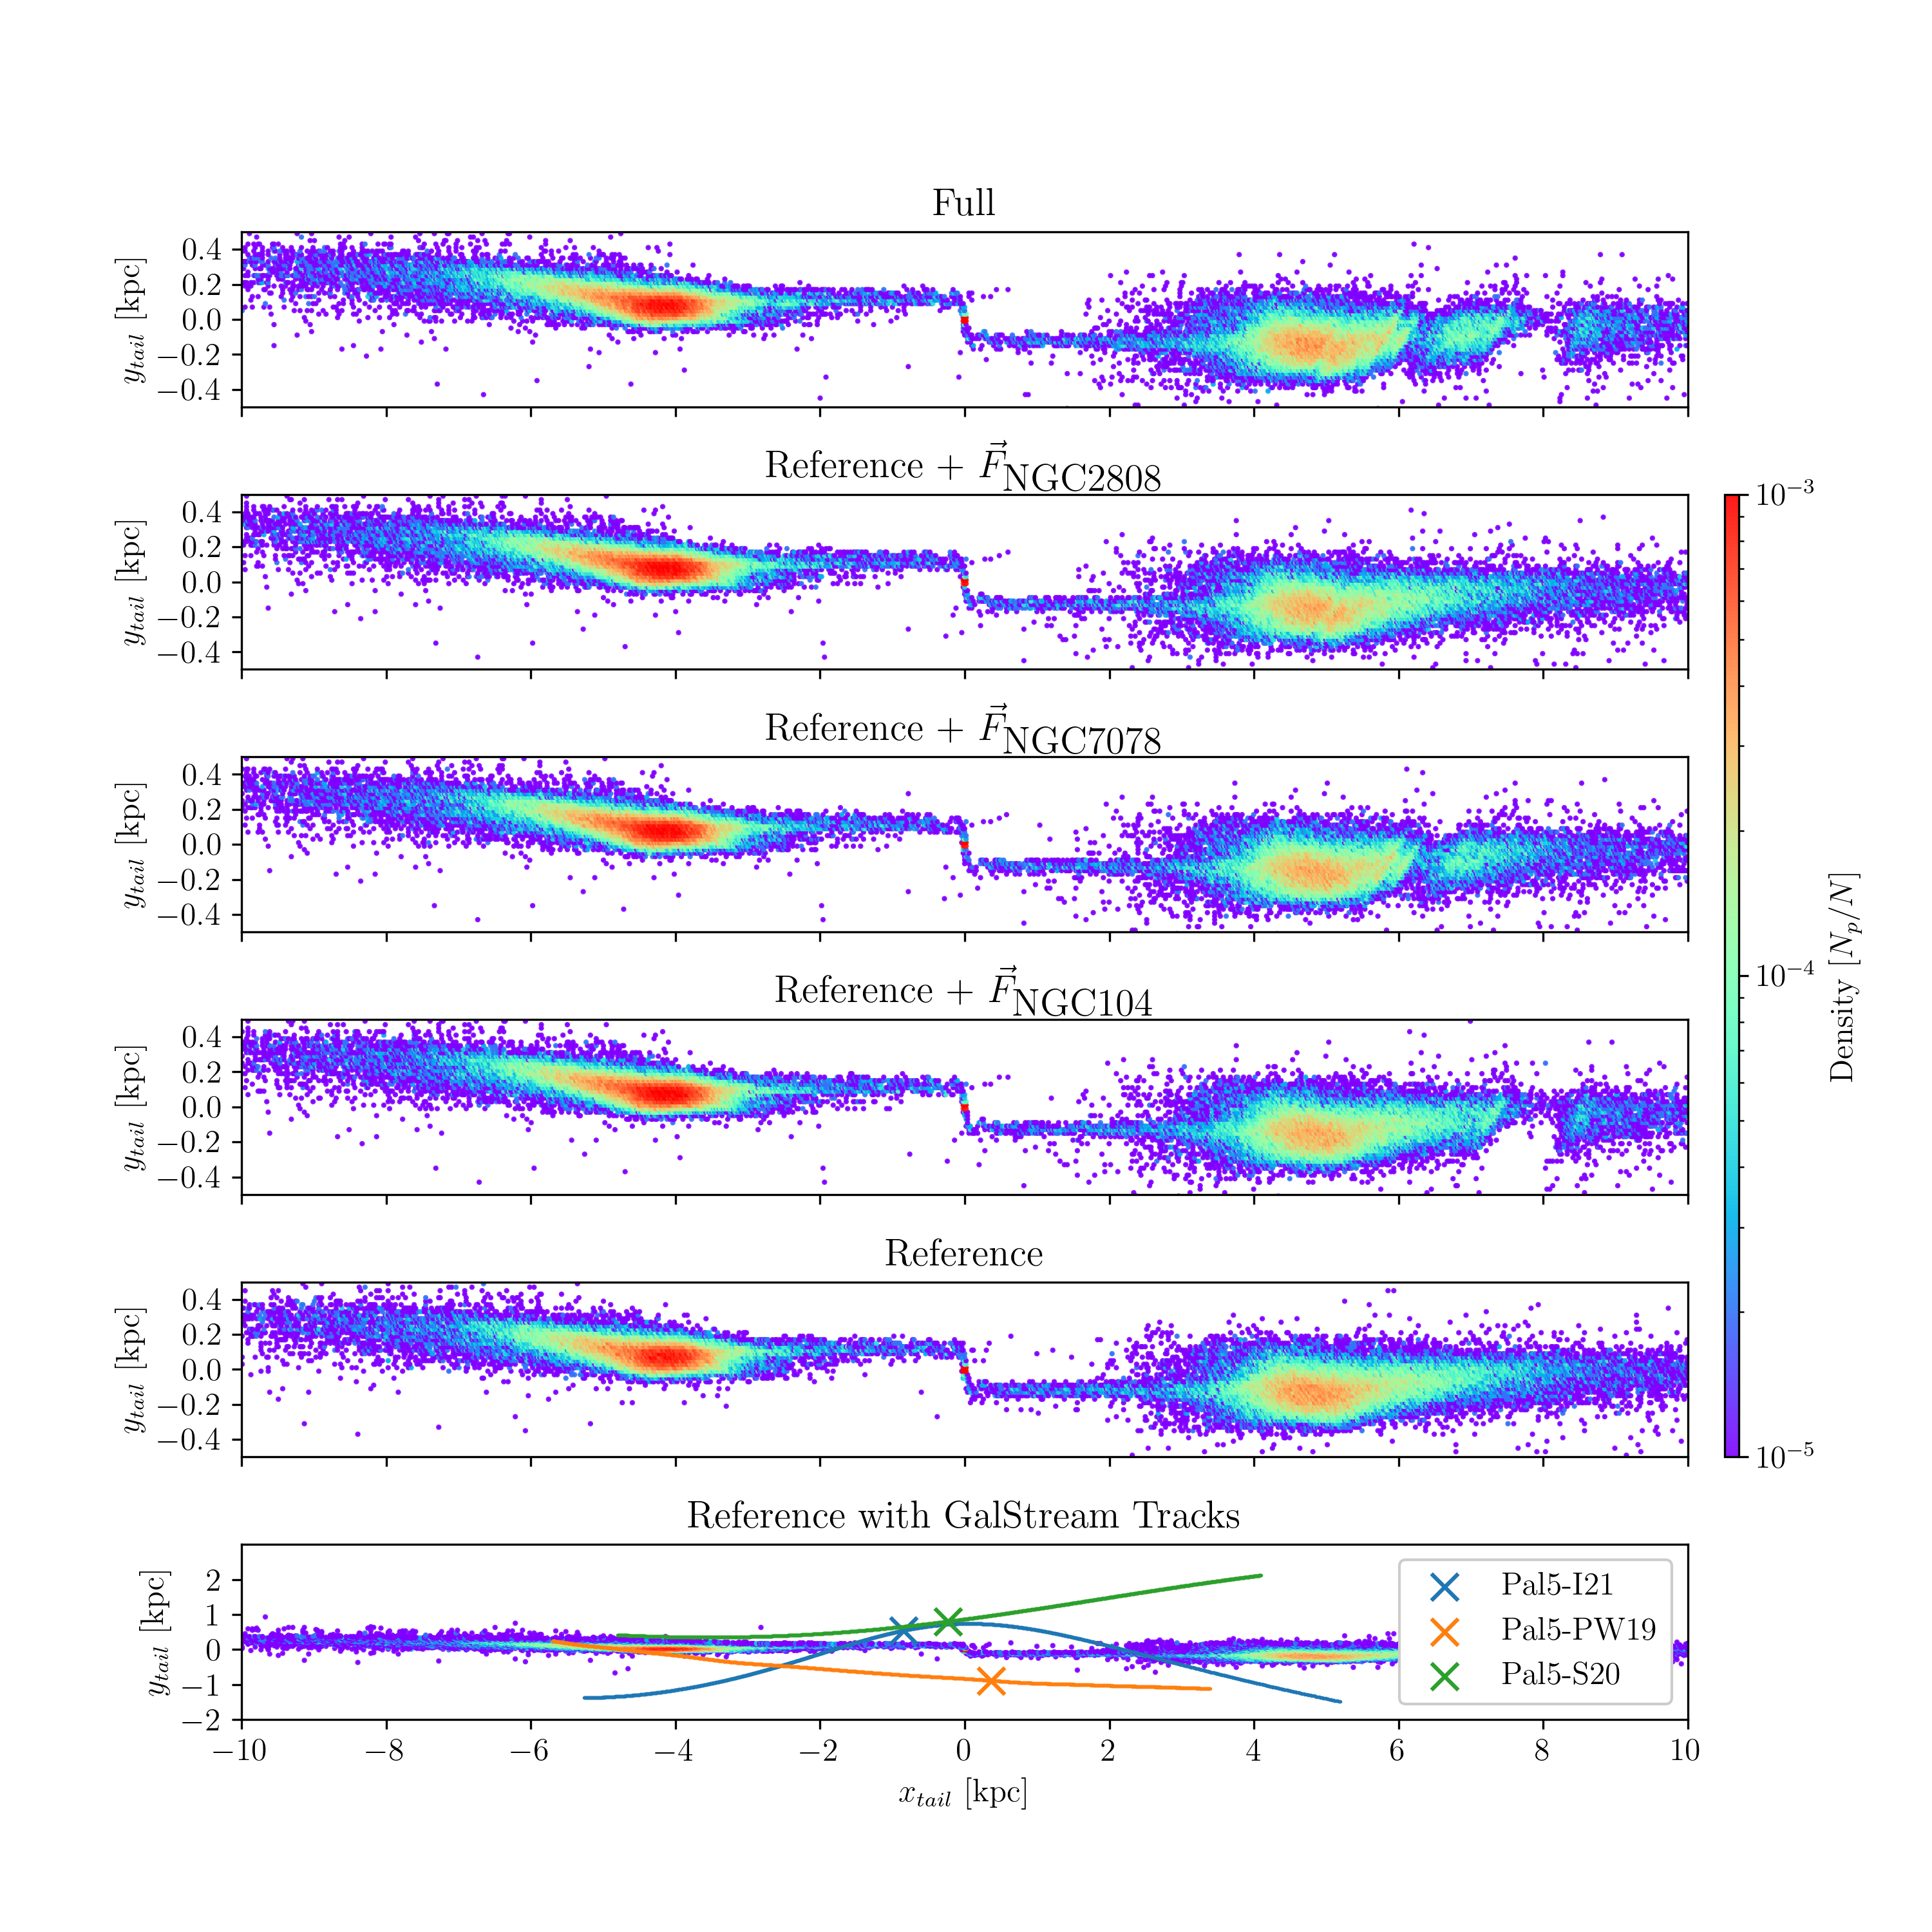
\includegraphics[width=\linewidth]{decomposition-monte-carlo-009-with-3-gaps.png}
    \caption[]{This figure decomposes the gaps found in the full simulation to the responsible perturbers. The pertuber candidates were found in Fig.~\ref{fig:profiles}, and extra simulations were run in which we singularly add the suspects to verify that it was indeed them who created the gaps. The titles explain which simulation is which, and there's also a descrepandy map. (I think I'm going to get rid of the DIFF map)}
    \label{fig:profiles}
    \end{figure*}  


  




  \begin{figure}
    \centering
    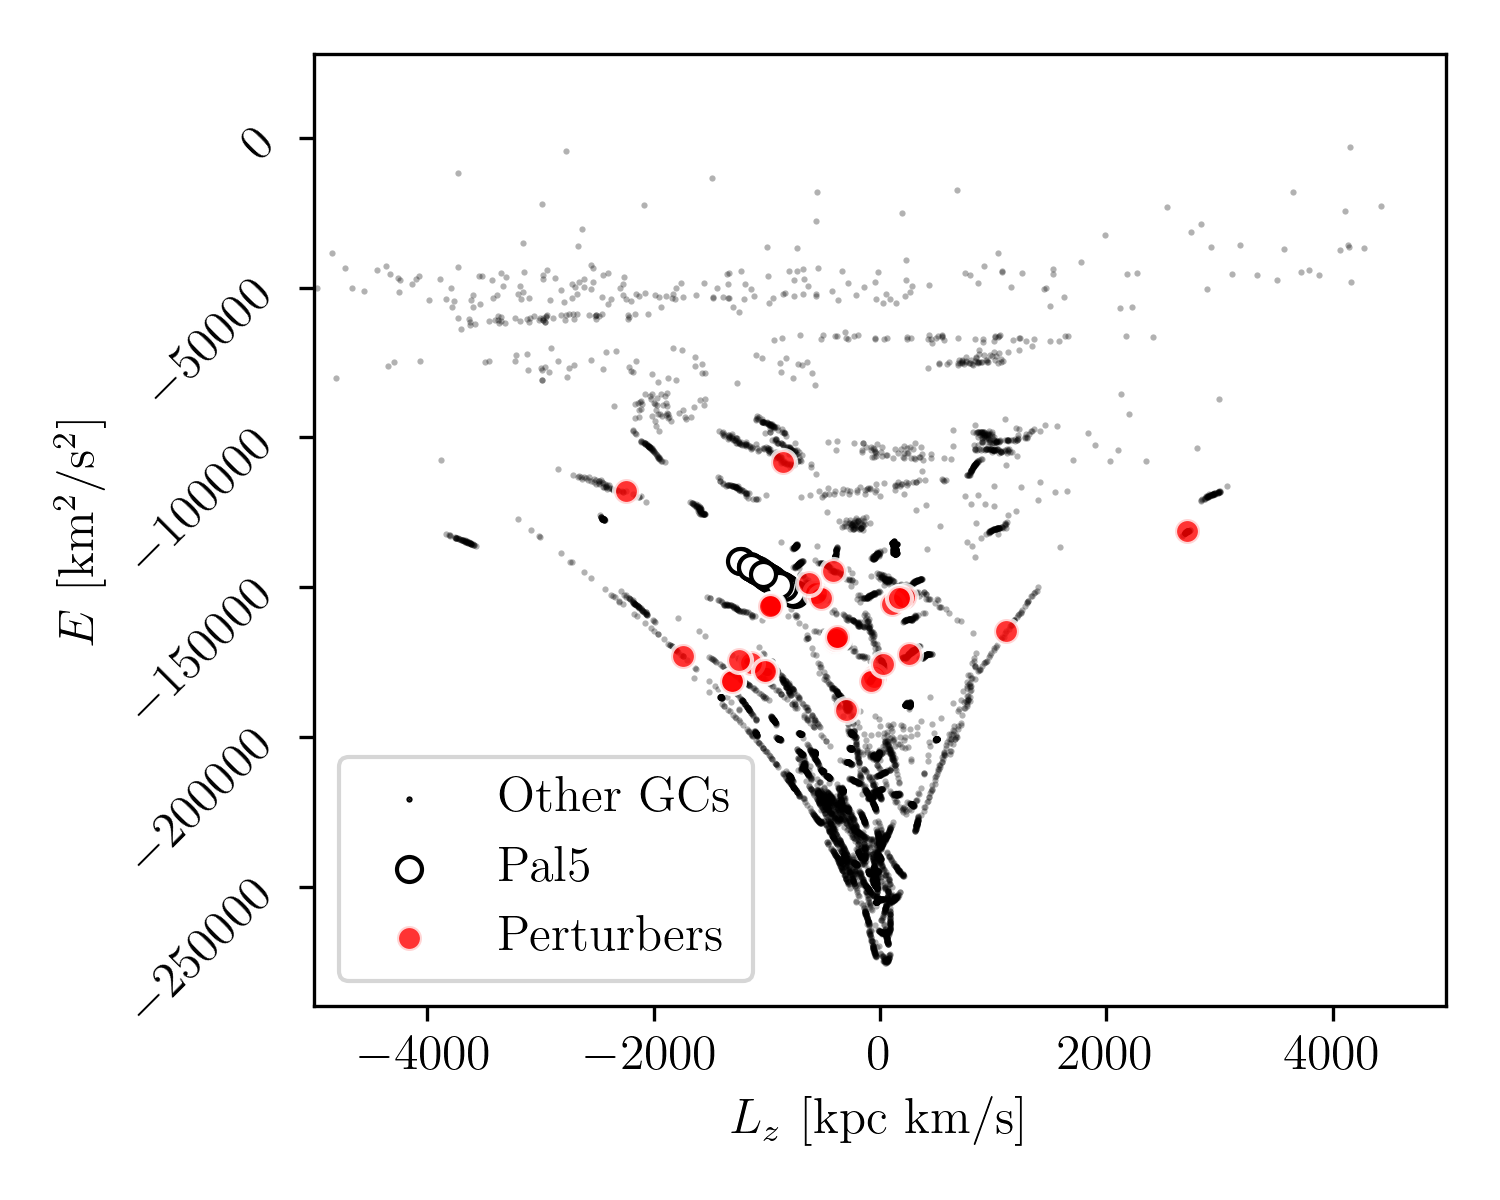
\includegraphics[width=1\linewidth]{E_Lz_perturbers.png}
    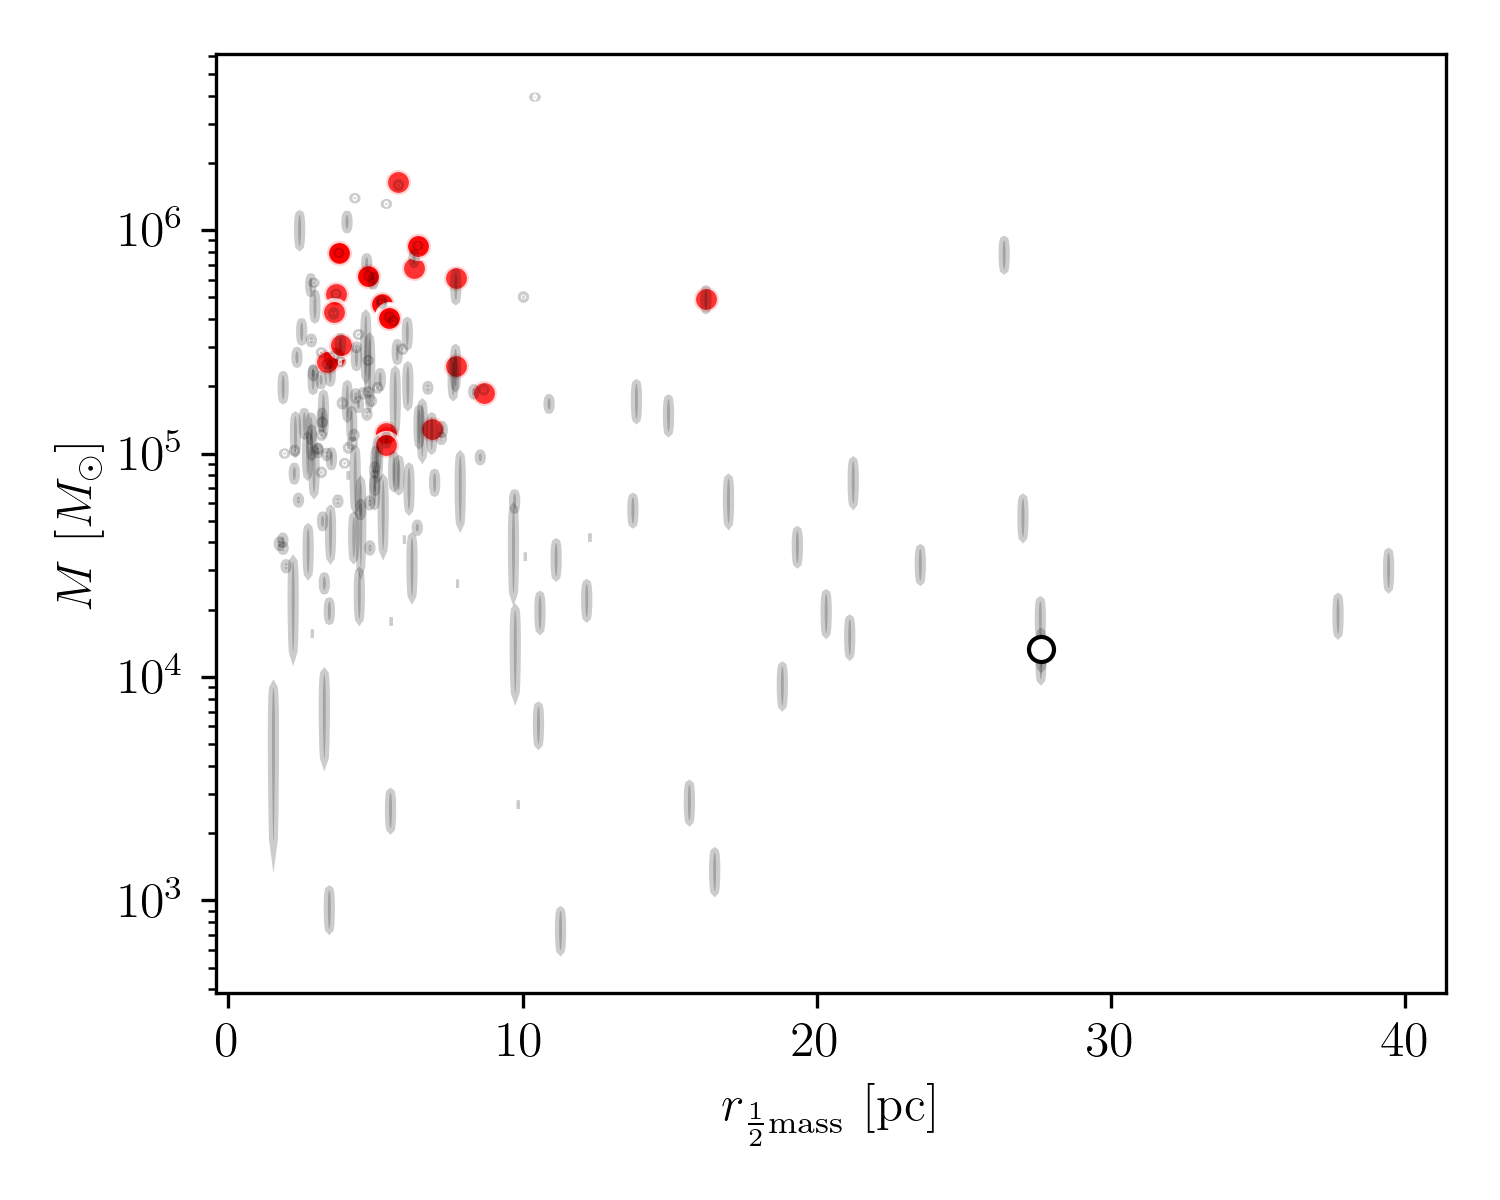
\includegraphics[width=1\linewidth]{mass_size_plane.png}
    \caption{One plot shows the distribution in energy and angular momentum, the next are the inernal proeprties of the clusters, and the last show when the clusters commit their crime, and how many times it happens accross the 50 simulations. }
    \label{fig:mass_size_plane}
    \end{figure}
  \begin{figure*}
    \centering
    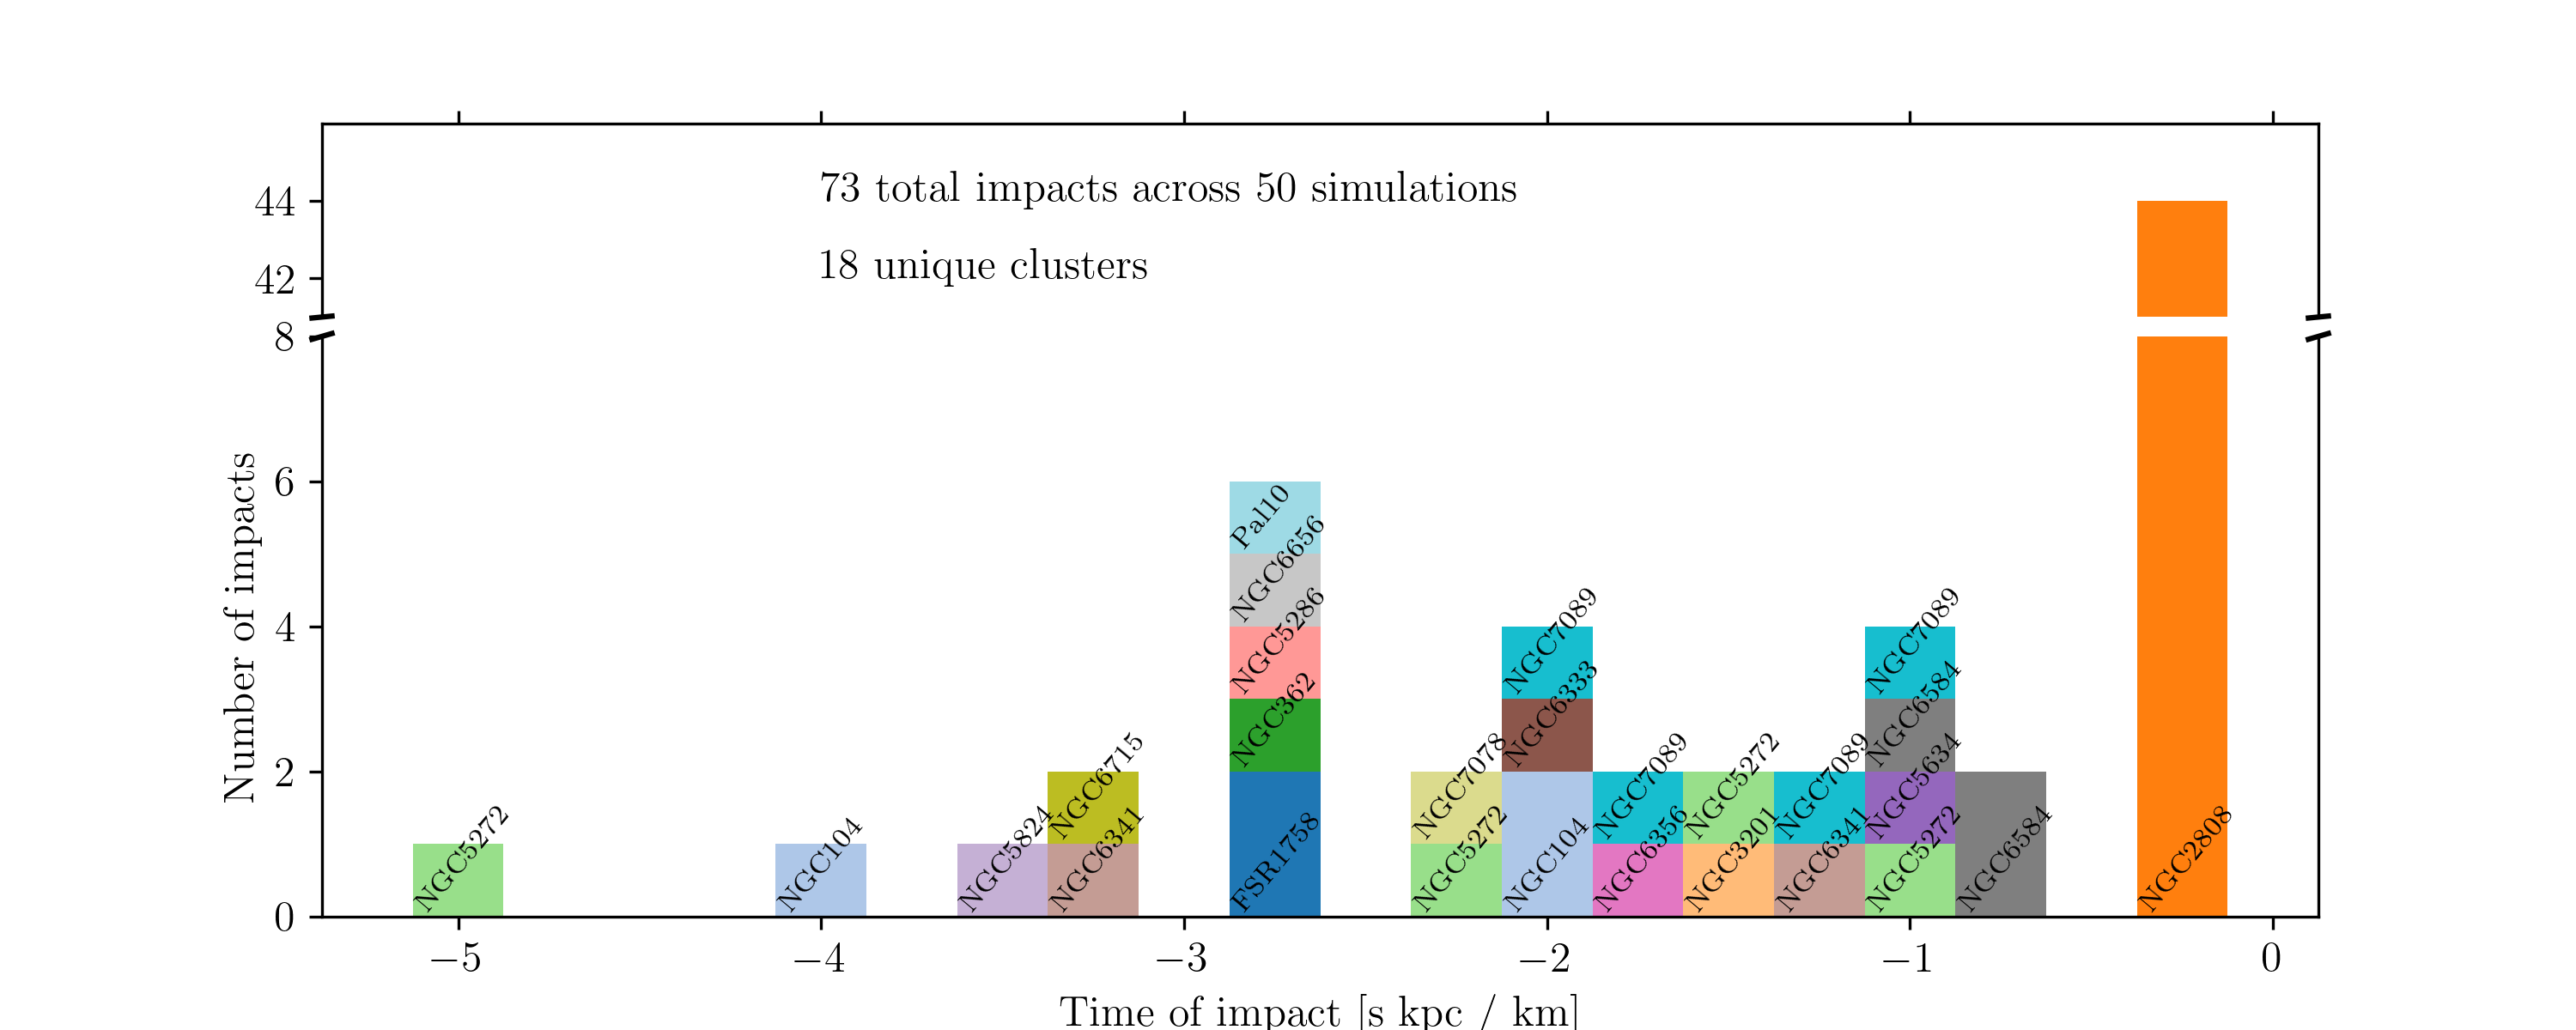
\includegraphics[width=\linewidth]{histogram_impact_time.png}
    \caption{When the impacts occured}
    \label{fig:histogram_impact_time}
    \end{figure*}
  


  \section{Discussion}
    $10^5-10^6$. Sotto alone averbbero questo effetto? 





\bibliographystyle{aa} % or another style like plain, unsrt, etc.
\bibliography{bibliography} % replace 'references' with the name of your .bib file



\begin{appendix}

  \section{Tail Coordinates} \label{appendix:TailCoordinates}

  \begin{figure}
    \centering
    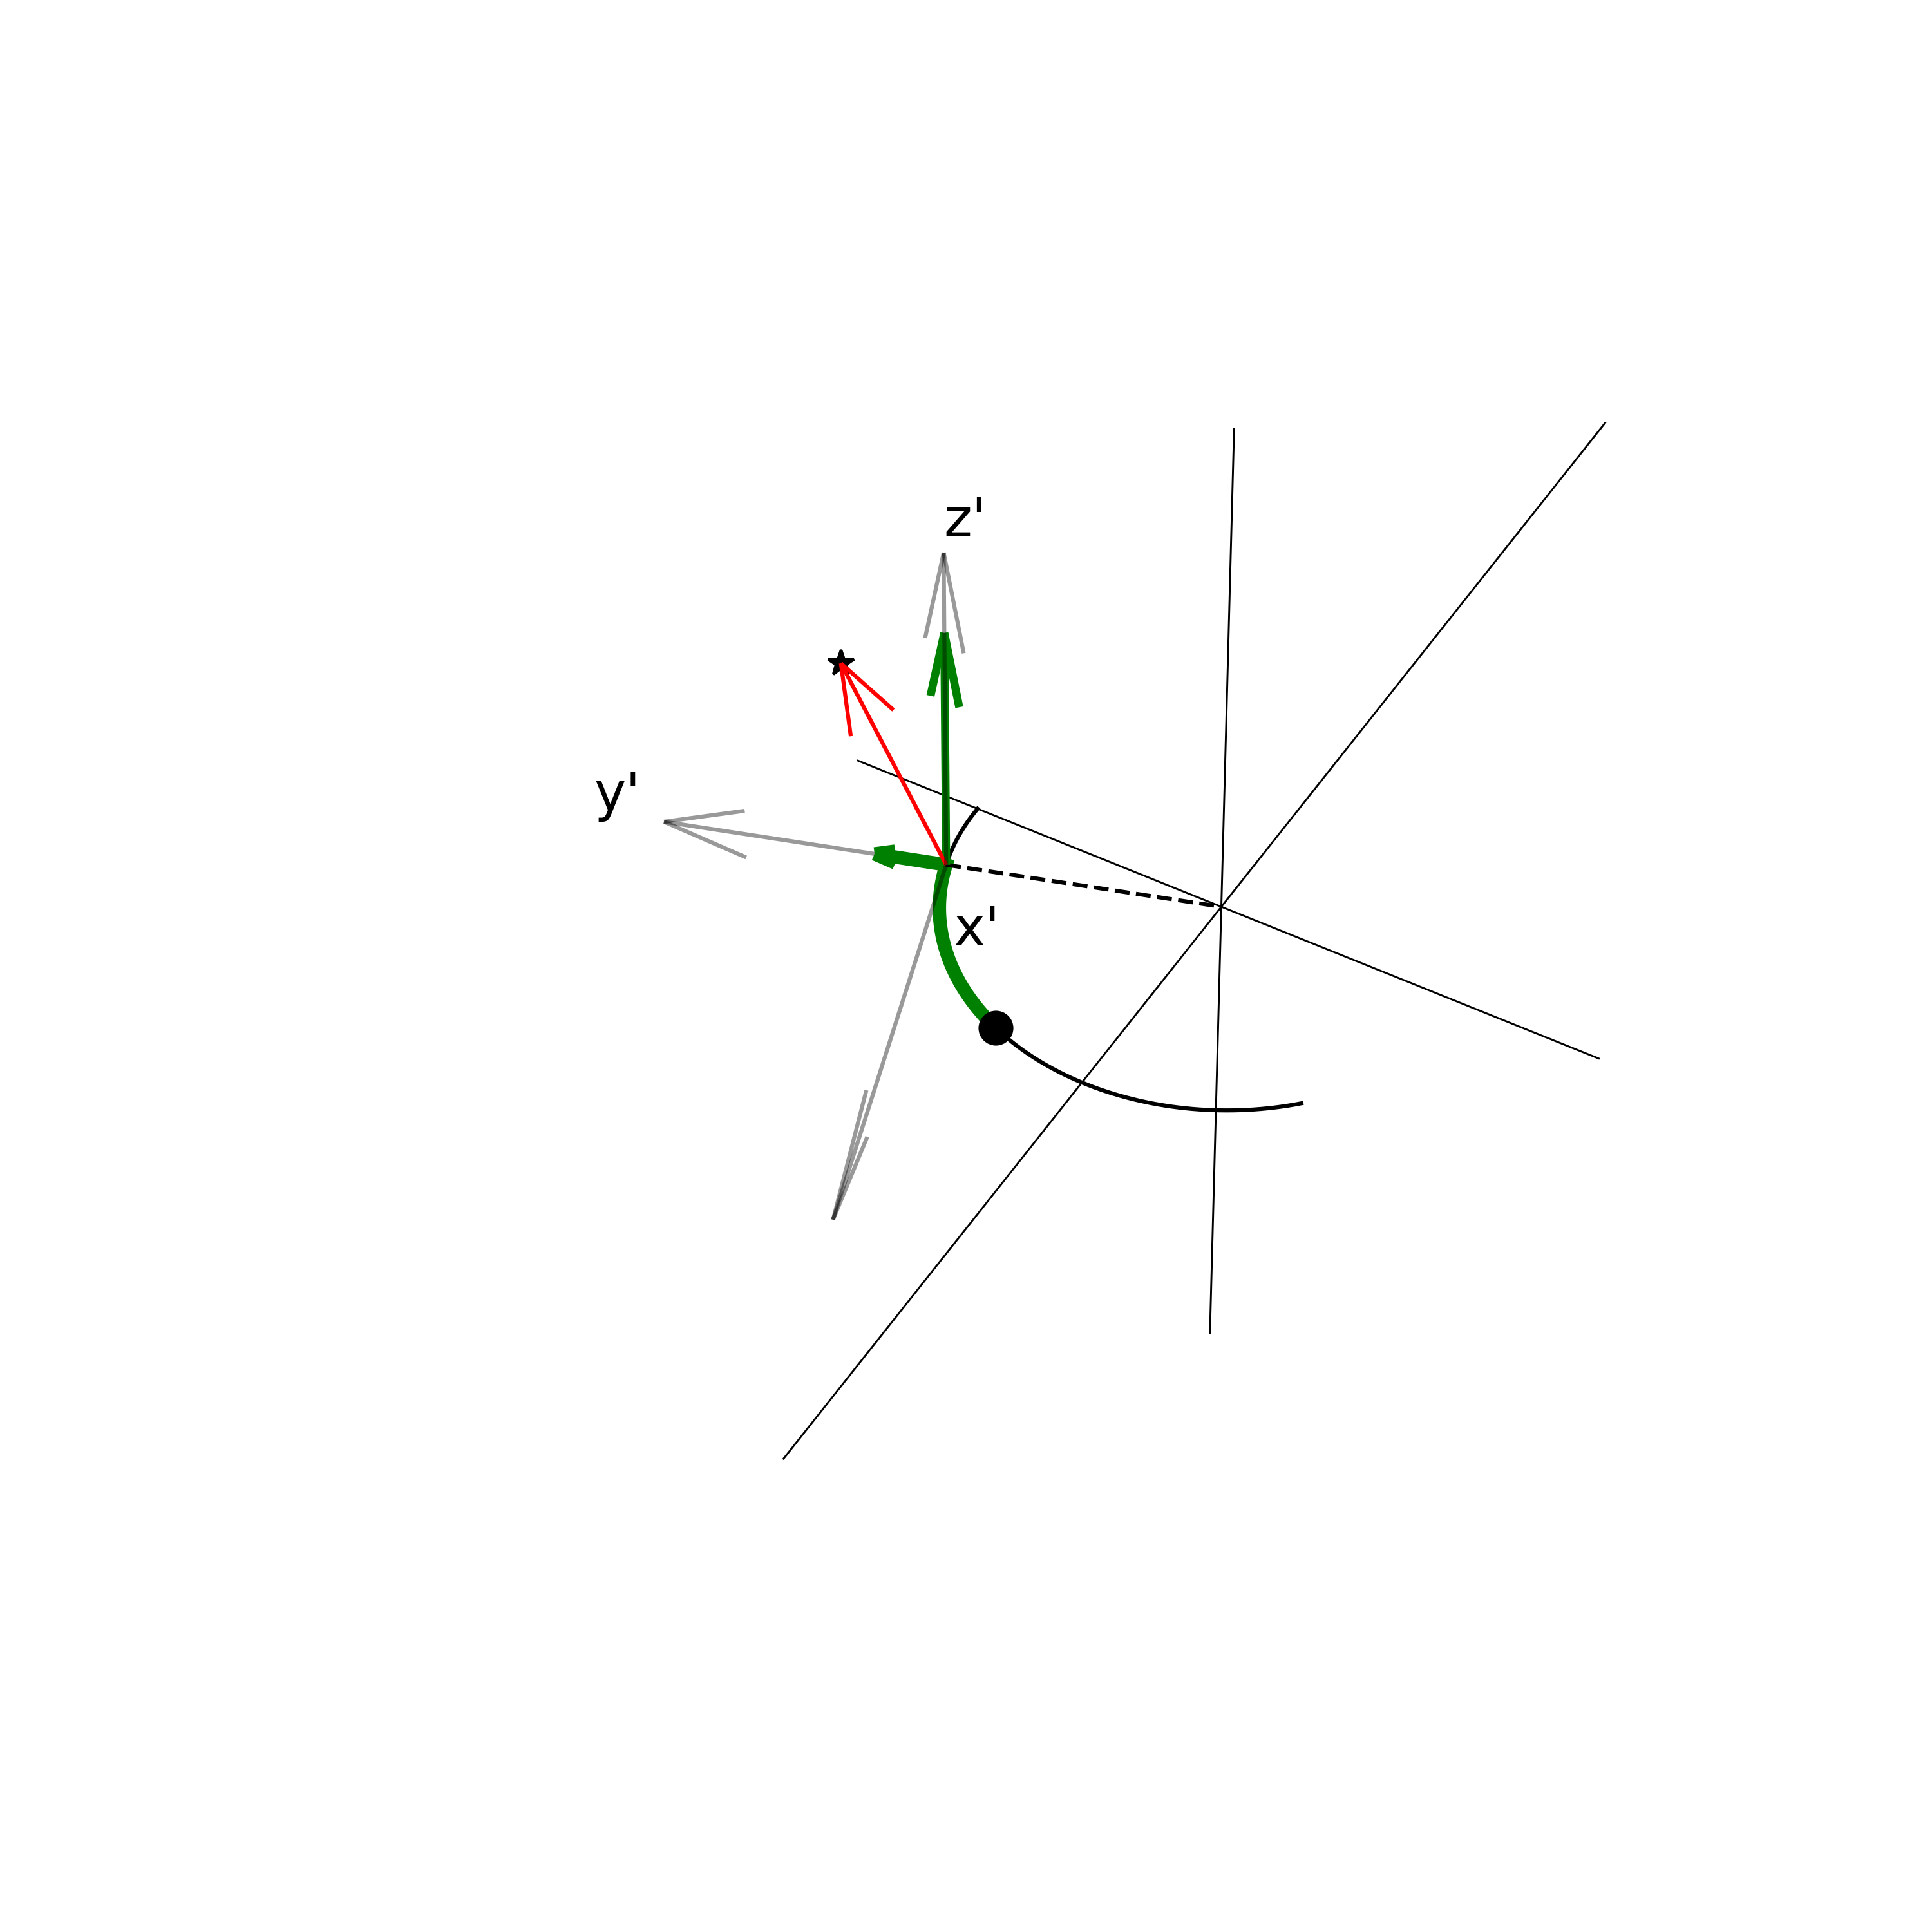
\includegraphics[width=\linewidth]{figures/along_orbit_coordinate_system-approved.png}
    \caption{Tail coordinates}
    \label{fig:TailCoordinates}
  \end{figure}




  \section{Gallery of Gaps}

    \begin{figure*}
      \centering
      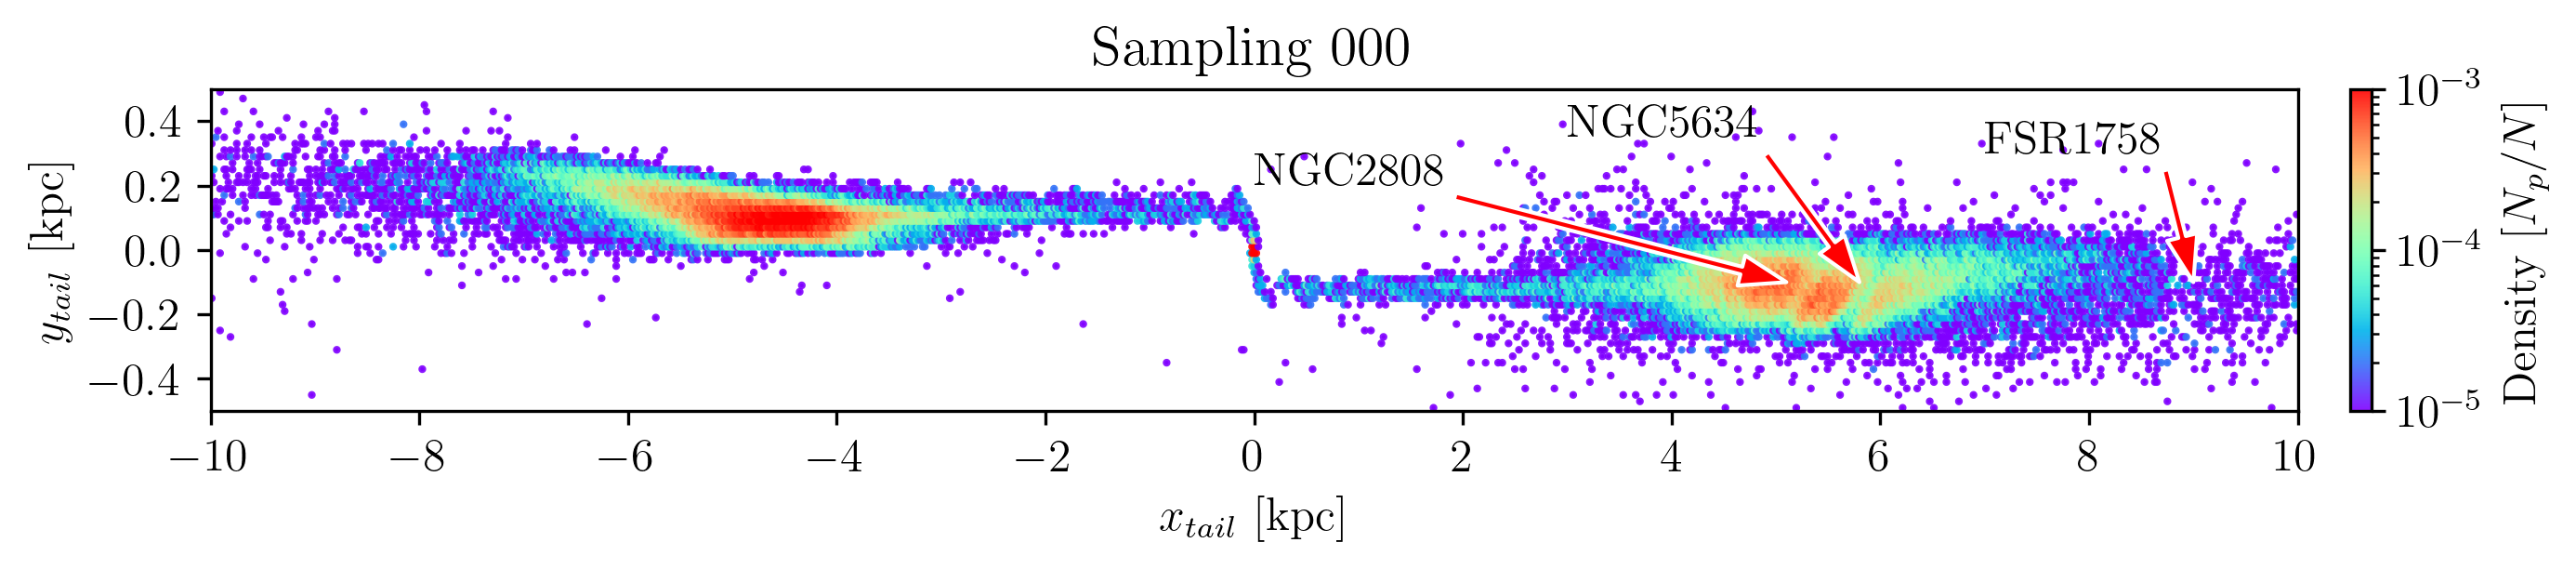
\includegraphics[width=\linewidth]{gallery_of_gaps_monte-carlo-000.png}
      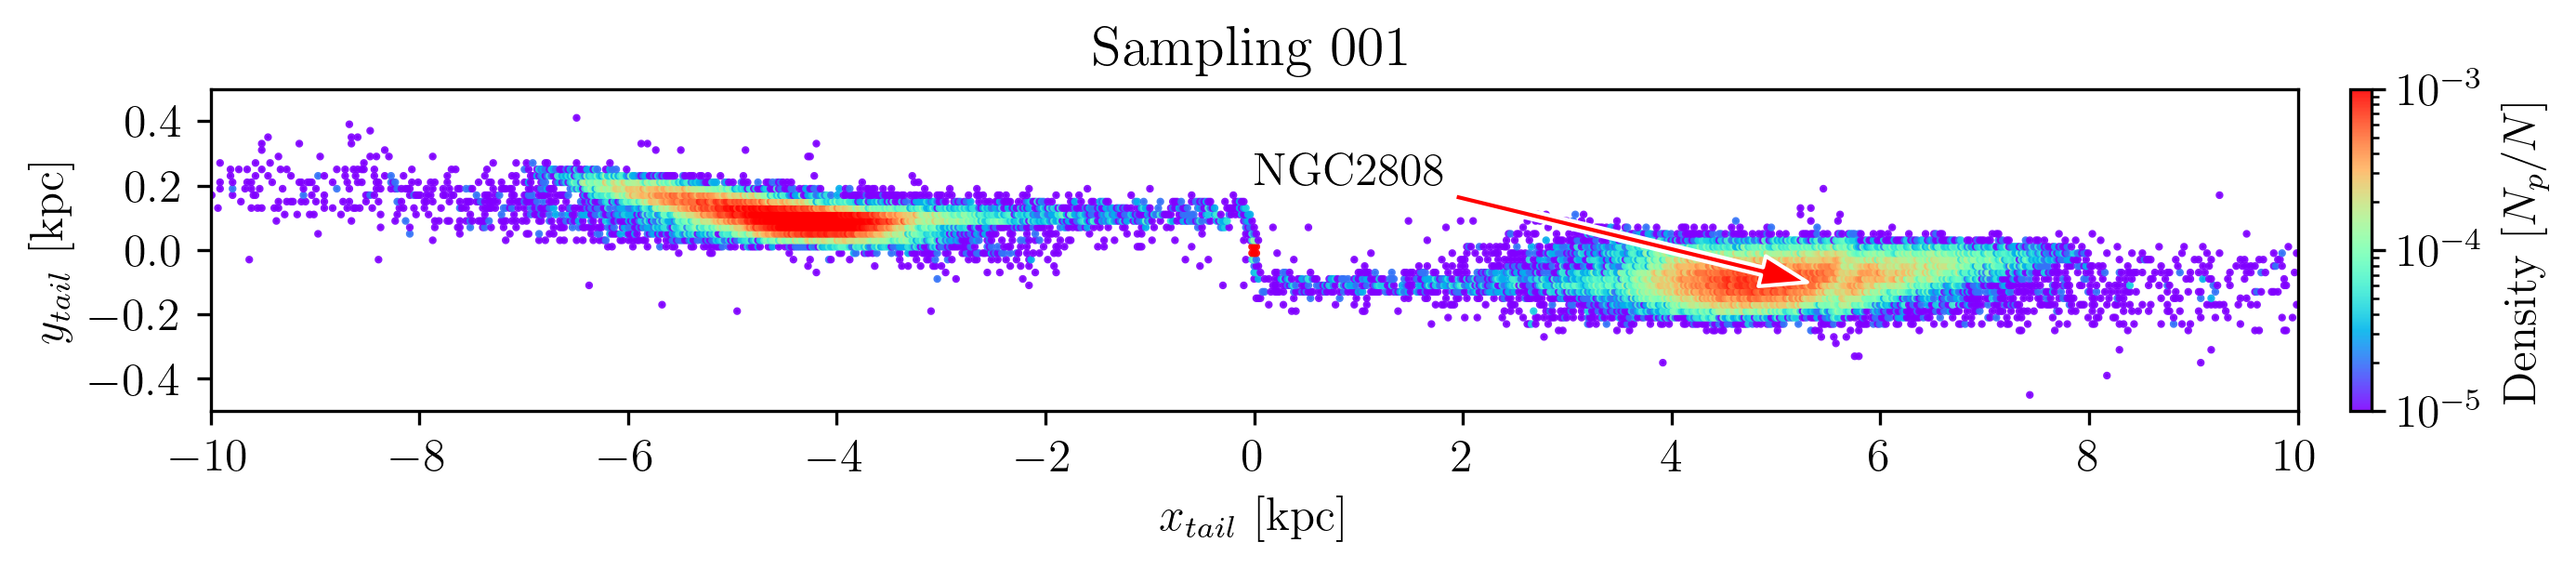
\includegraphics[width=\linewidth]{gallery_of_gaps_monte-carlo-001.png}
      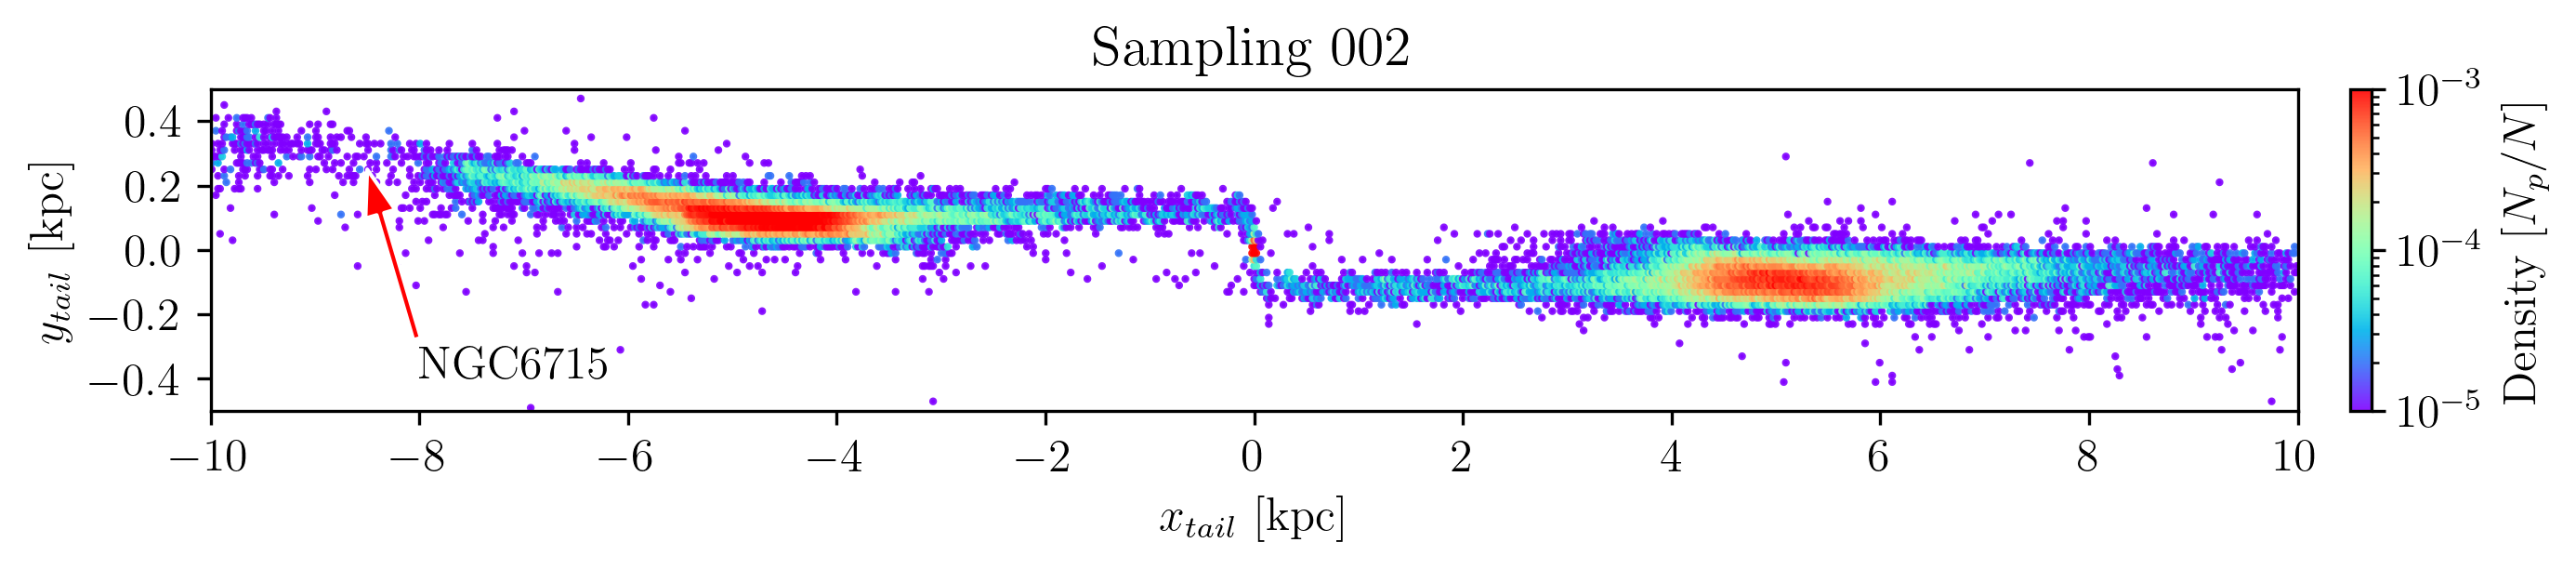
\includegraphics[width=\linewidth]{gallery_of_gaps_monte-carlo-002.png}
      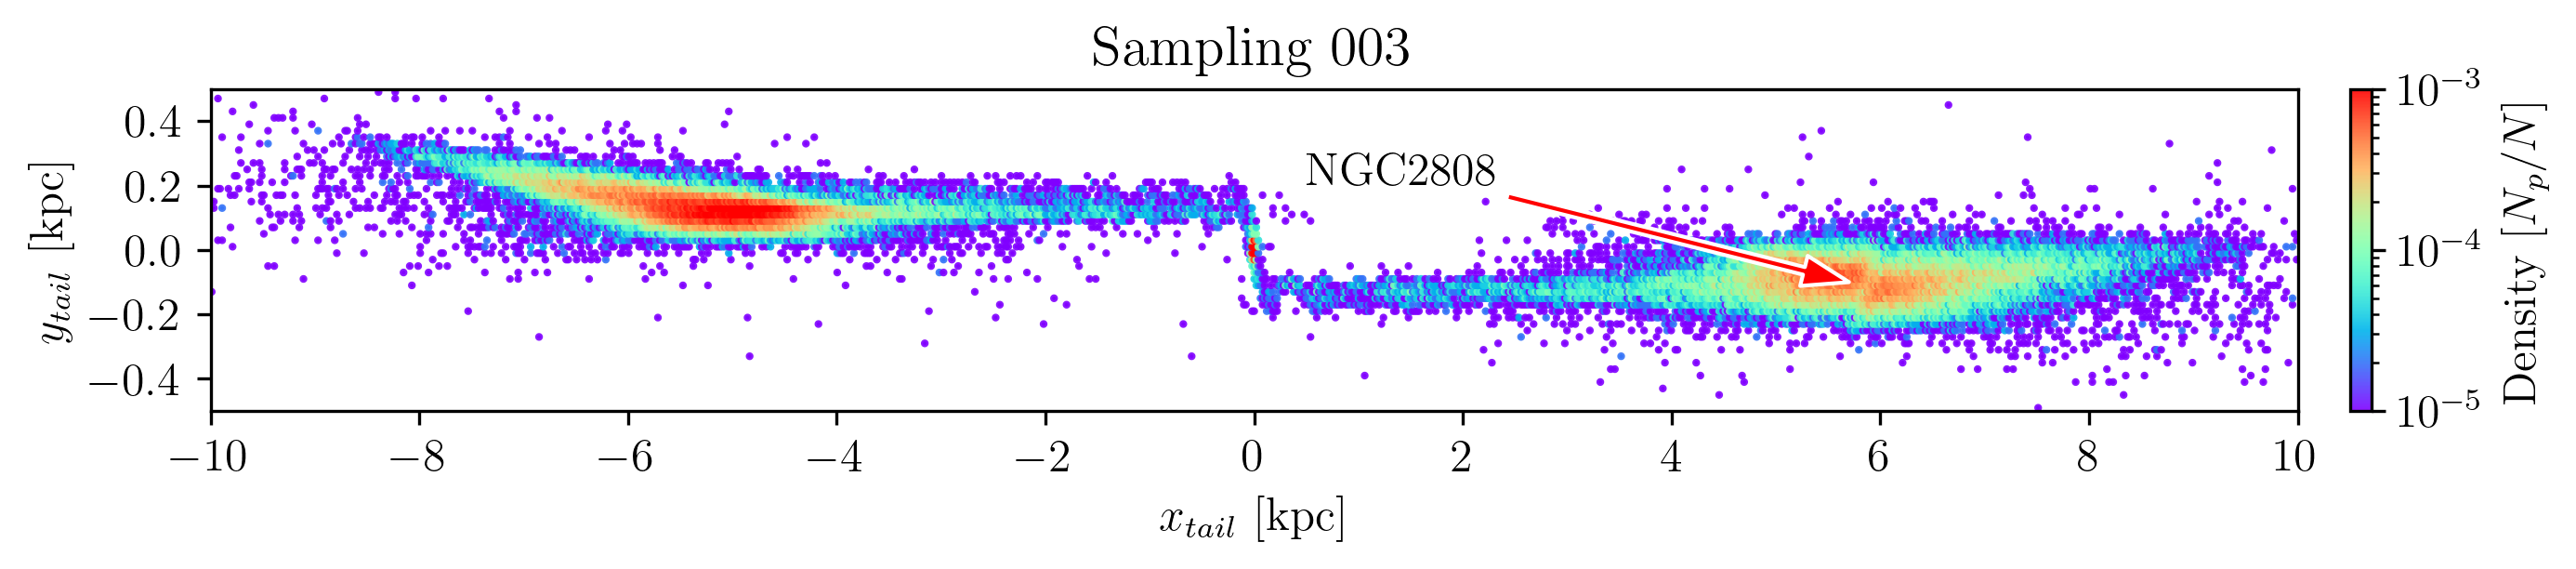
\includegraphics[width=\linewidth]{gallery_of_gaps_monte-carlo-003.png}
      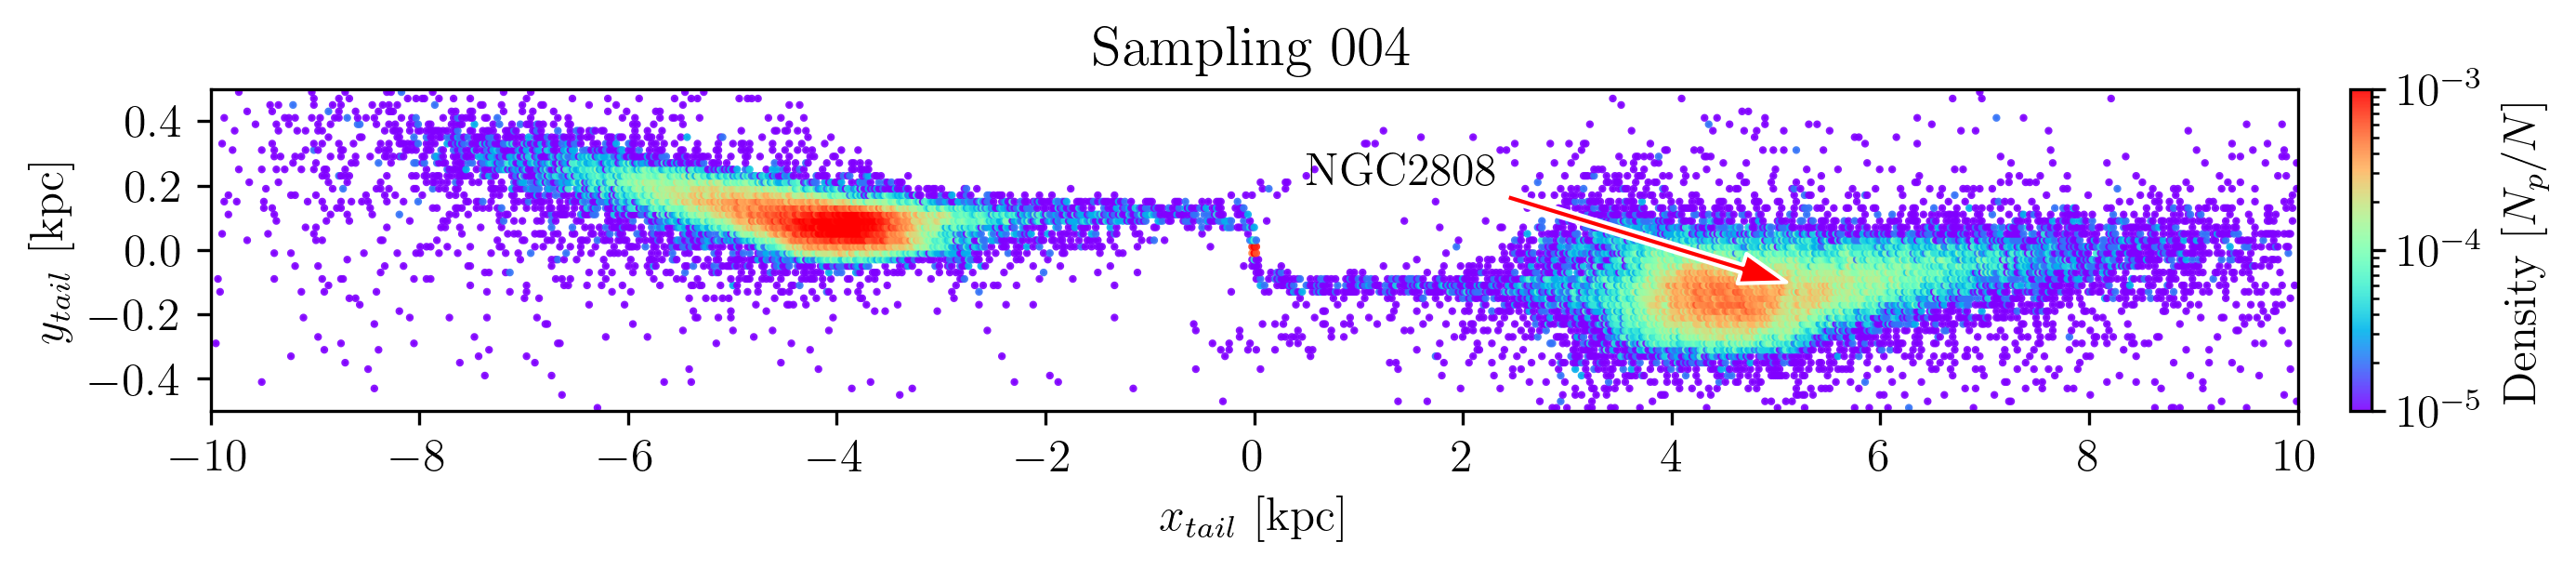
\includegraphics[width=\linewidth]{gallery_of_gaps_monte-carlo-004.png}
      \caption{Gap Gallery}
      \label{fig:TailCoordinates}
    \end{figure*}    


    \begin{figure*}
      \centering
      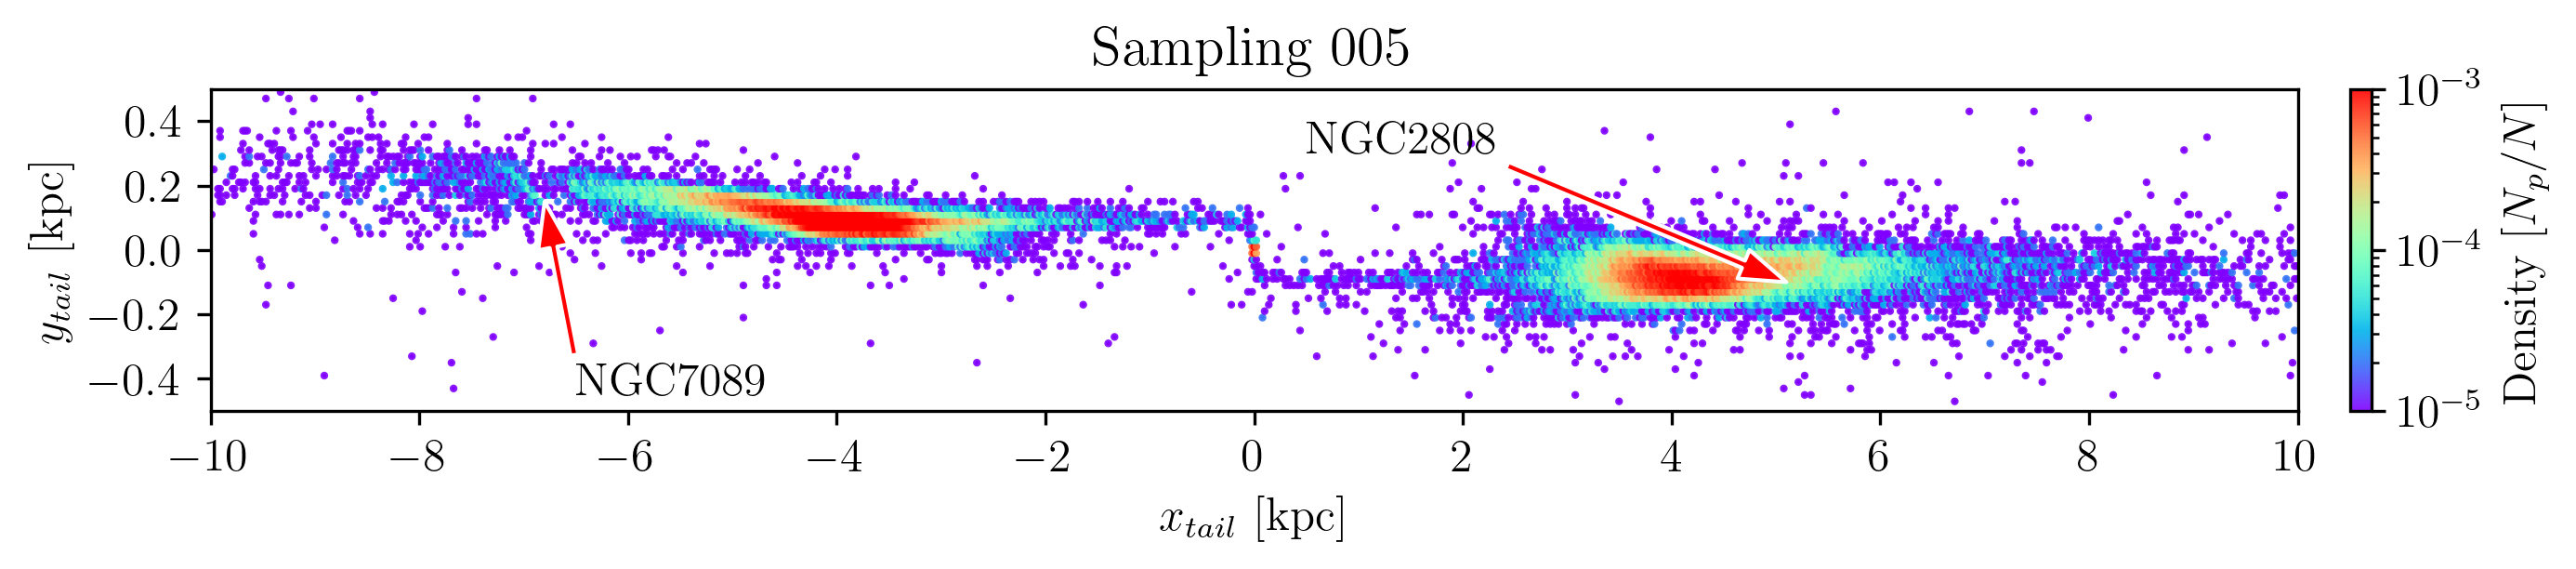
\includegraphics[width=\linewidth]{gallery_of_gaps_monte-carlo-005.png}
      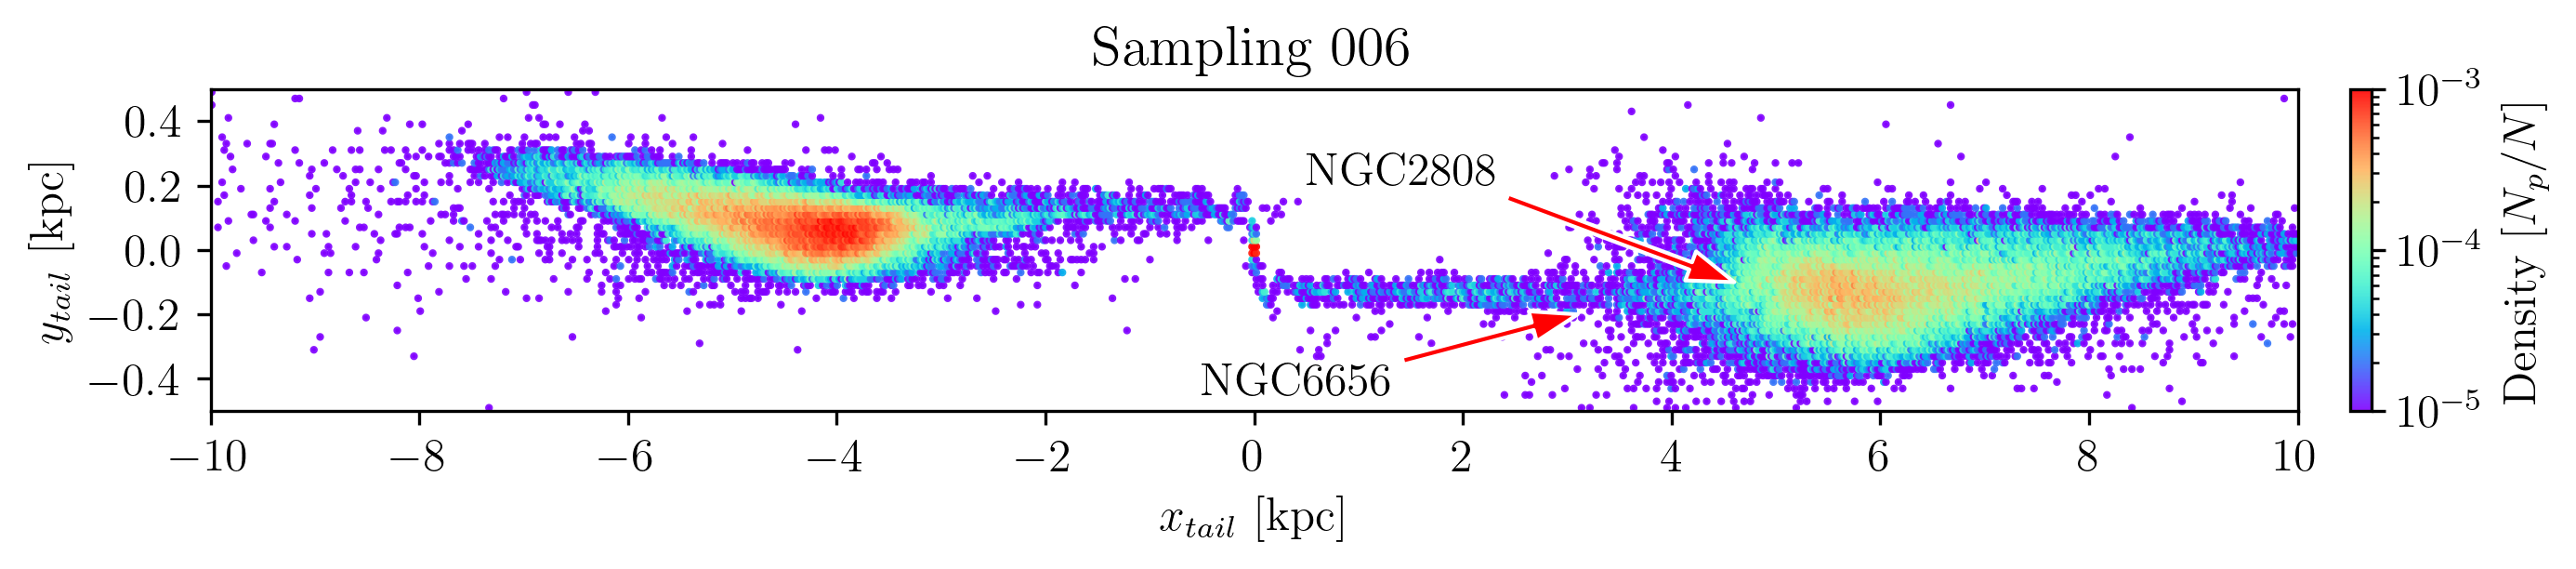
\includegraphics[width=\linewidth]{gallery_of_gaps_monte-carlo-006.png}
      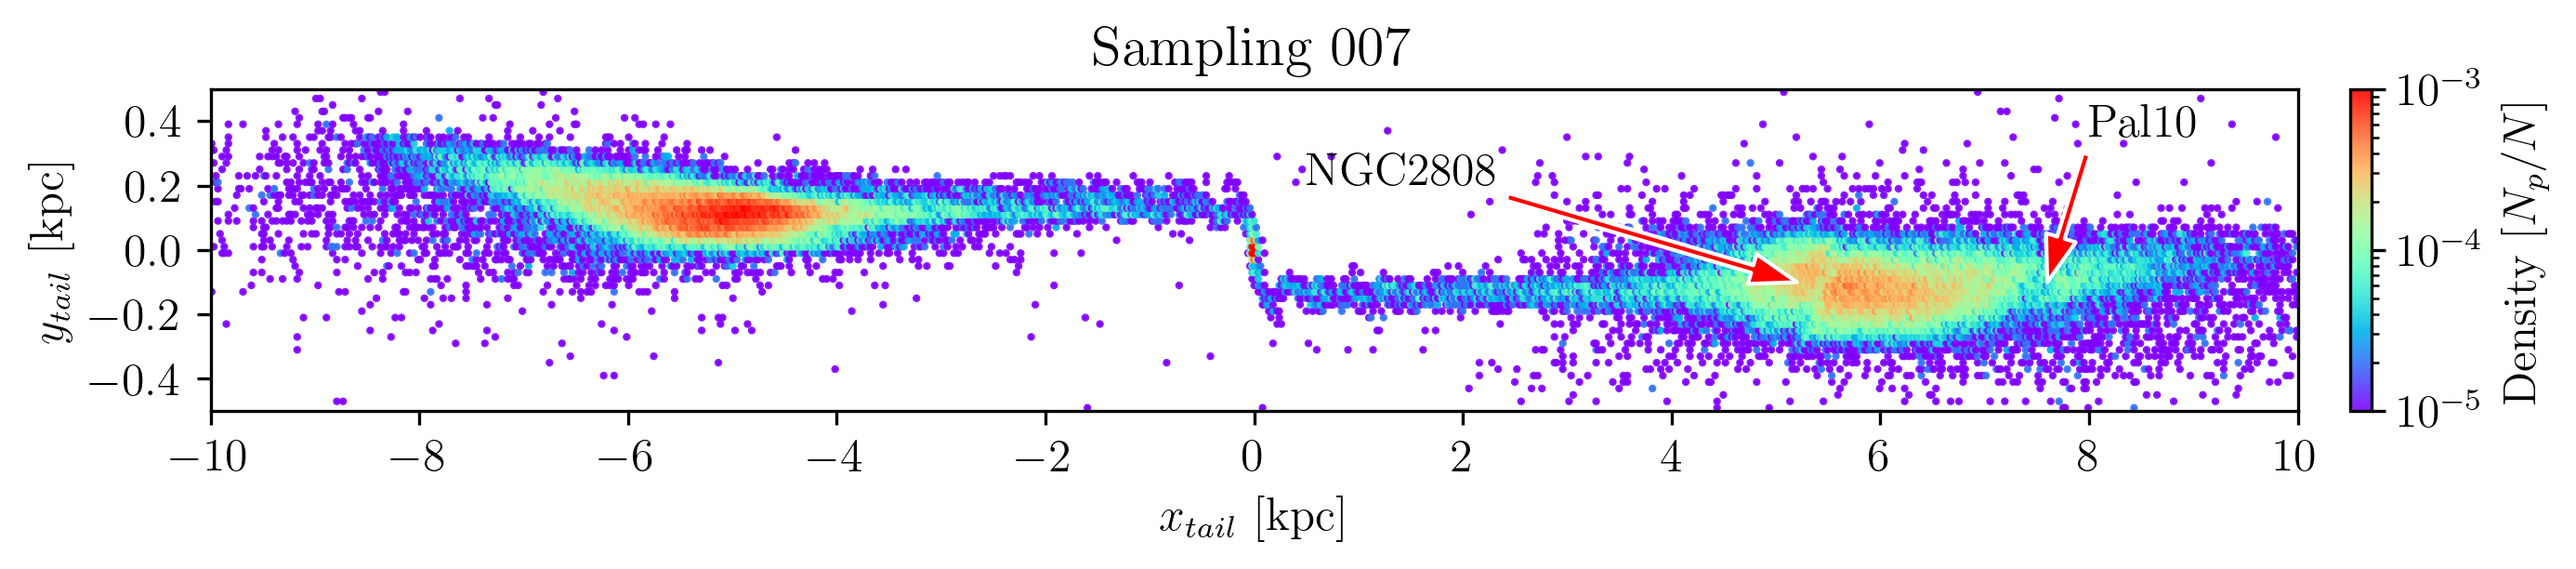
\includegraphics[width=\linewidth]{gallery_of_gaps_monte-carlo-007.png}
      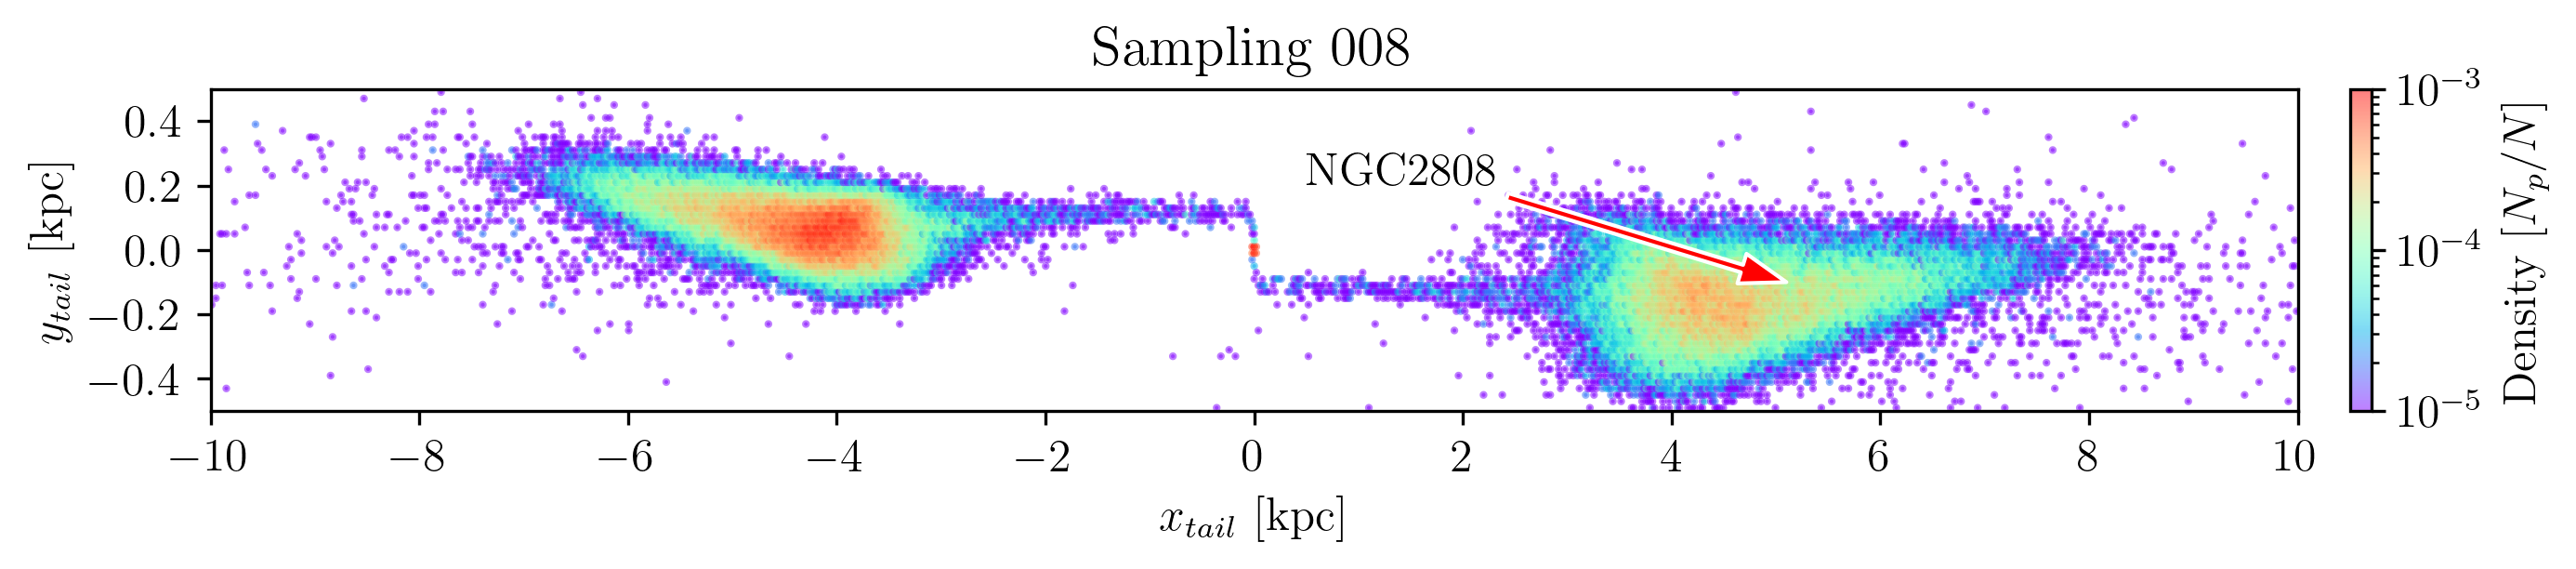
\includegraphics[width=\linewidth]{gallery_of_gaps_monte-carlo-008.png}
      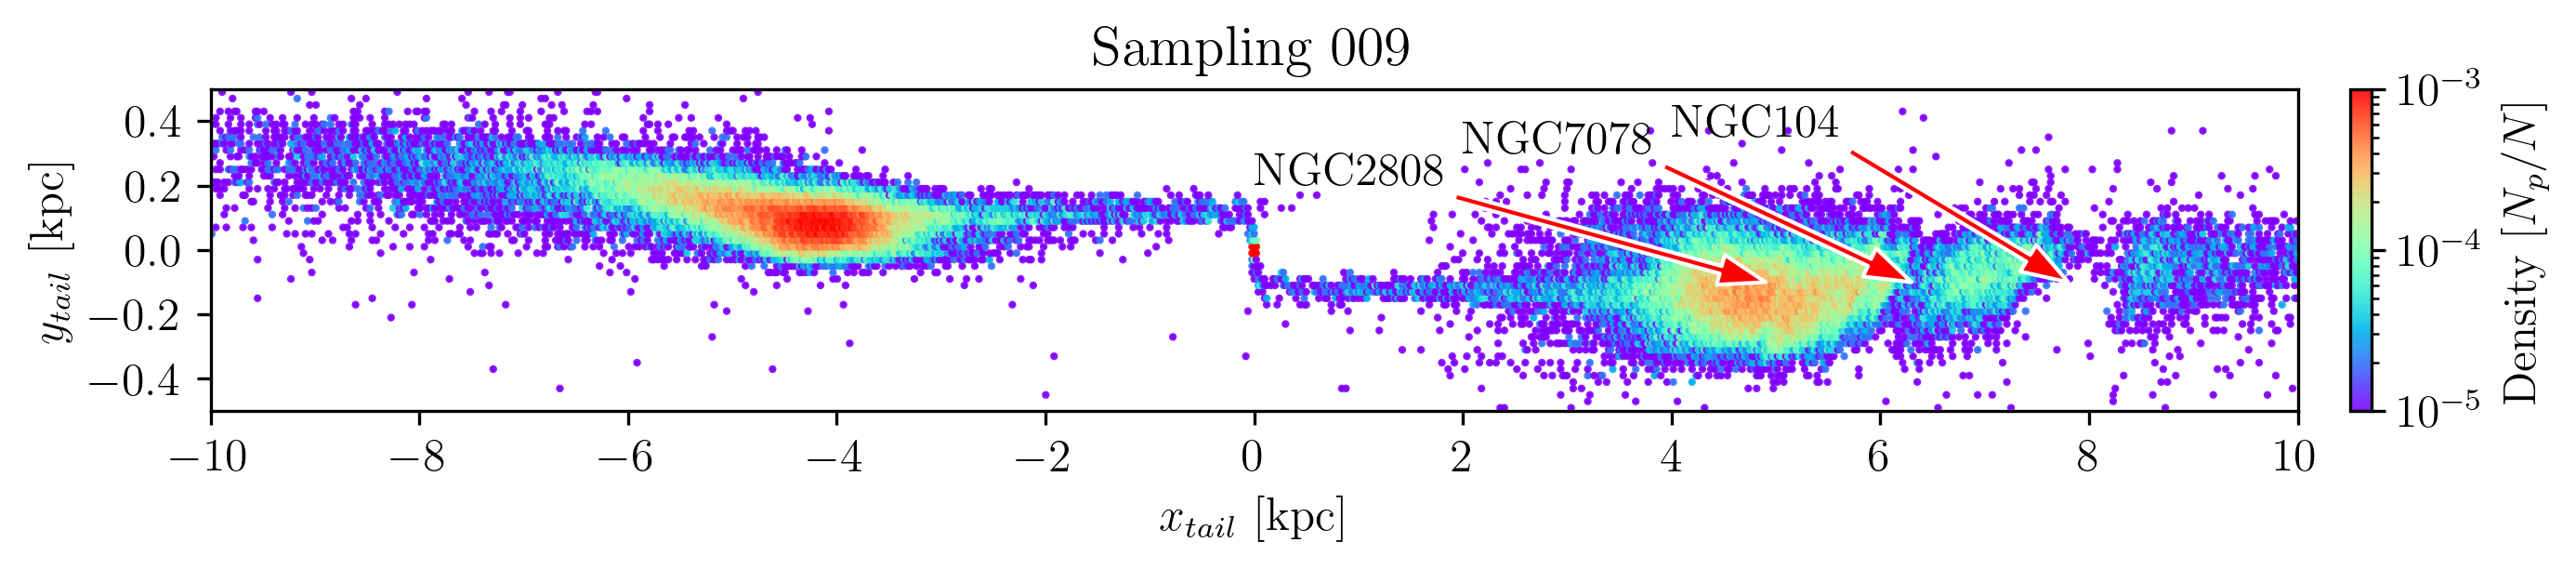
\includegraphics[width=\linewidth]{gallery_of_gaps_monte-carlo-009.png}
      \caption{Gap Gallery}
      \label{fig:TailCoordinates}
    \end{figure*}        


    \begin{figure*}
      \centering
      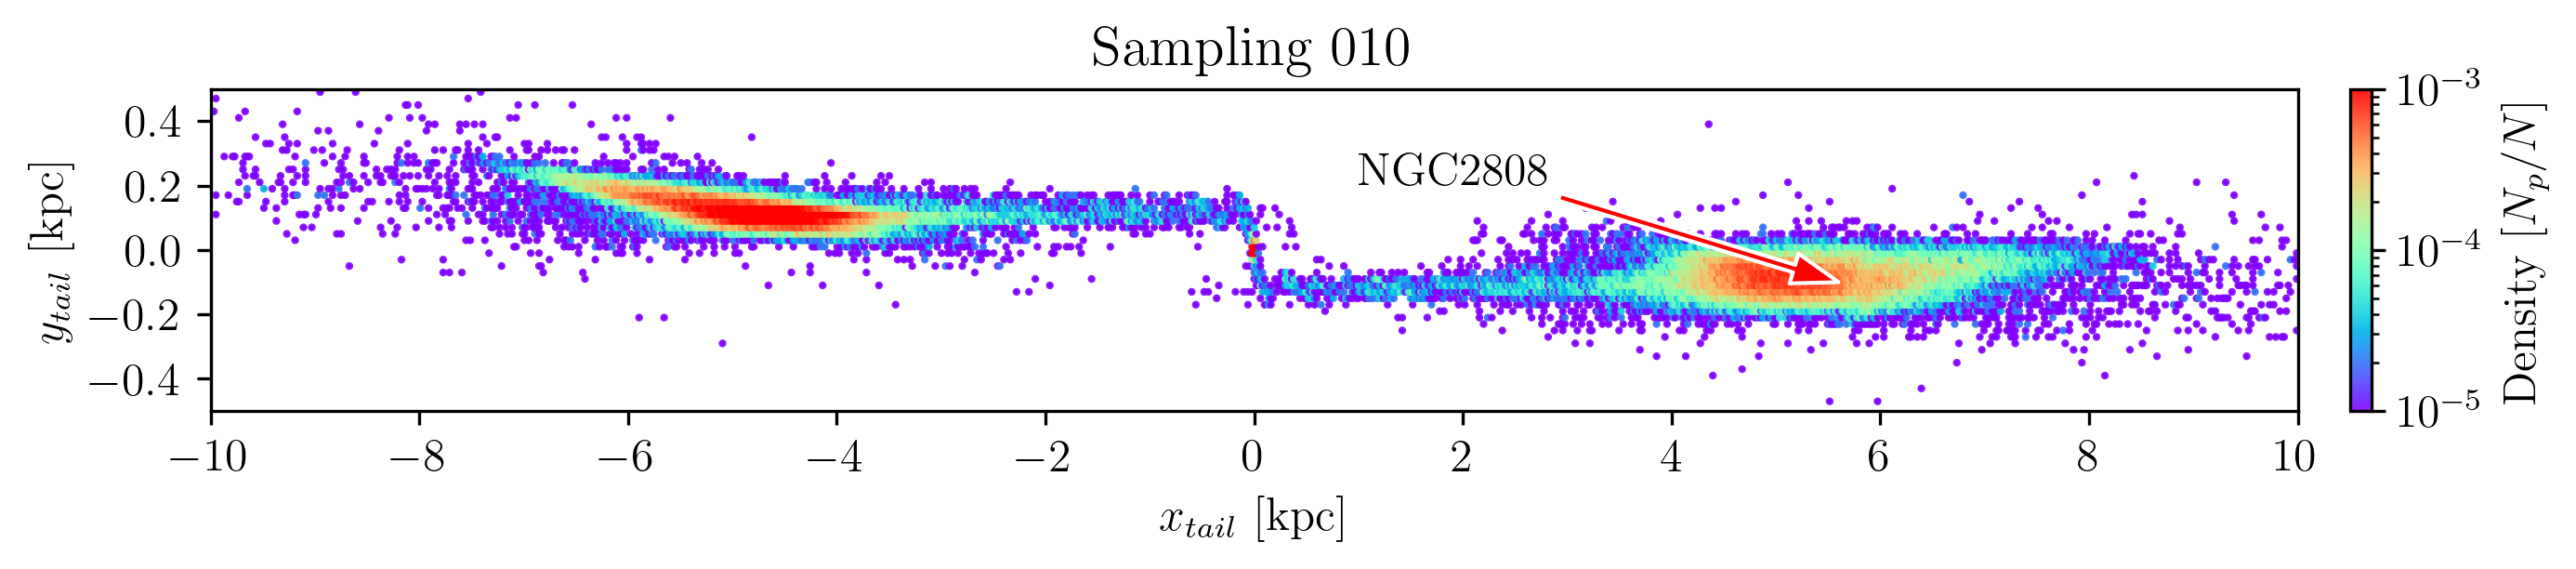
\includegraphics[width=\linewidth]{gallery_of_gaps_monte-carlo-010.png}
      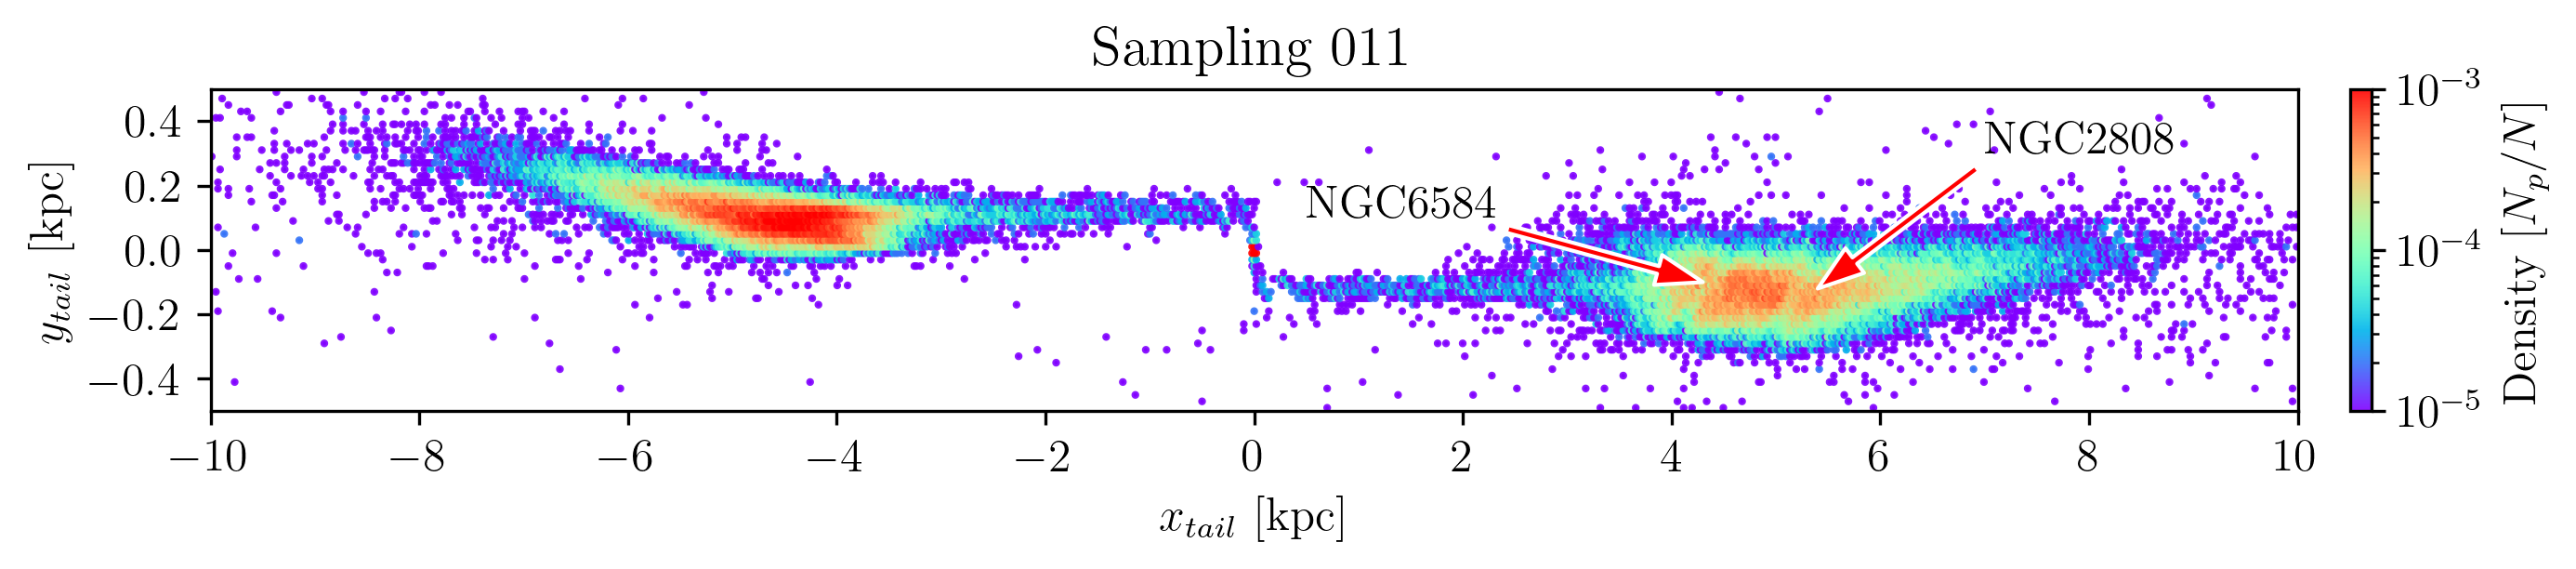
\includegraphics[width=\linewidth]{gallery_of_gaps_monte-carlo-011.png}
      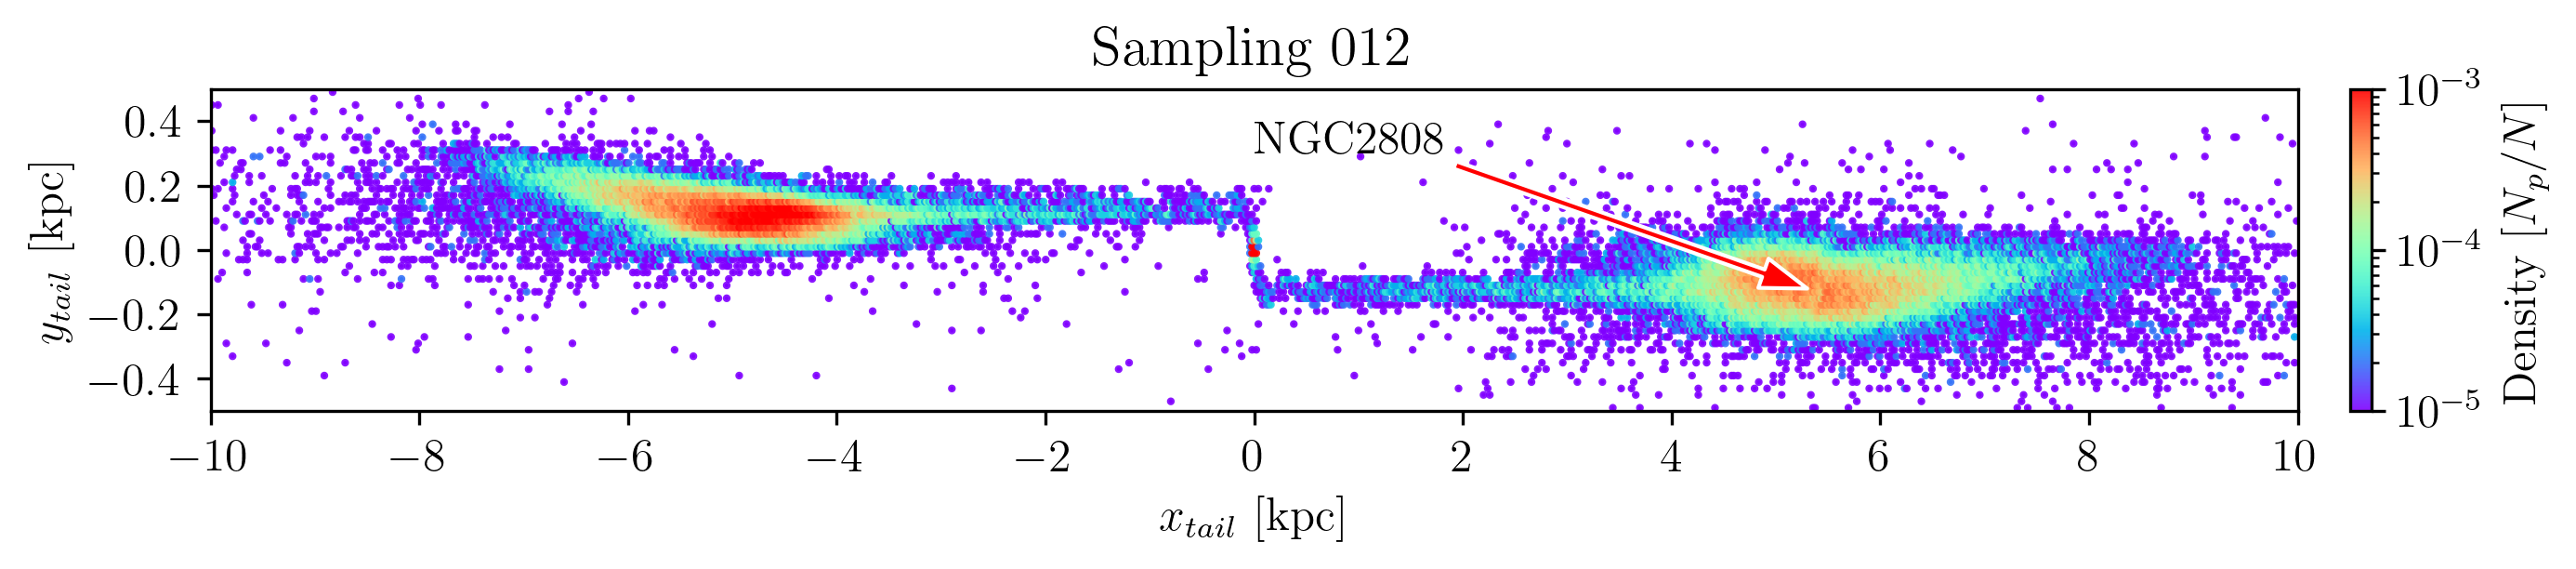
\includegraphics[width=\linewidth]{gallery_of_gaps_monte-carlo-012.png}
      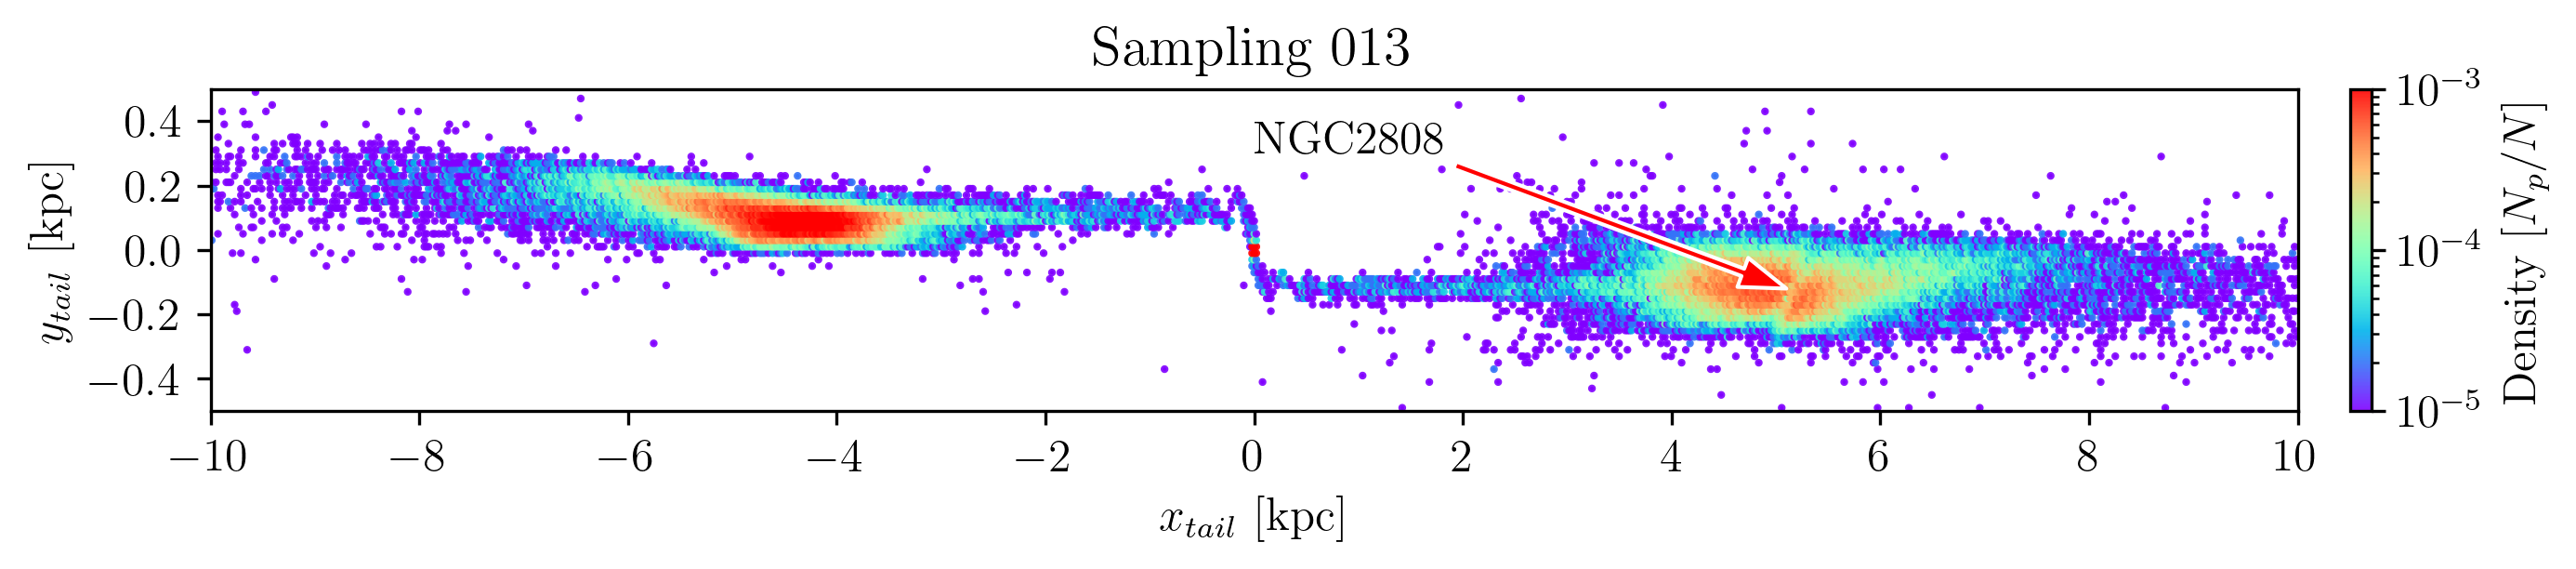
\includegraphics[width=\linewidth]{gallery_of_gaps_monte-carlo-013.png}
      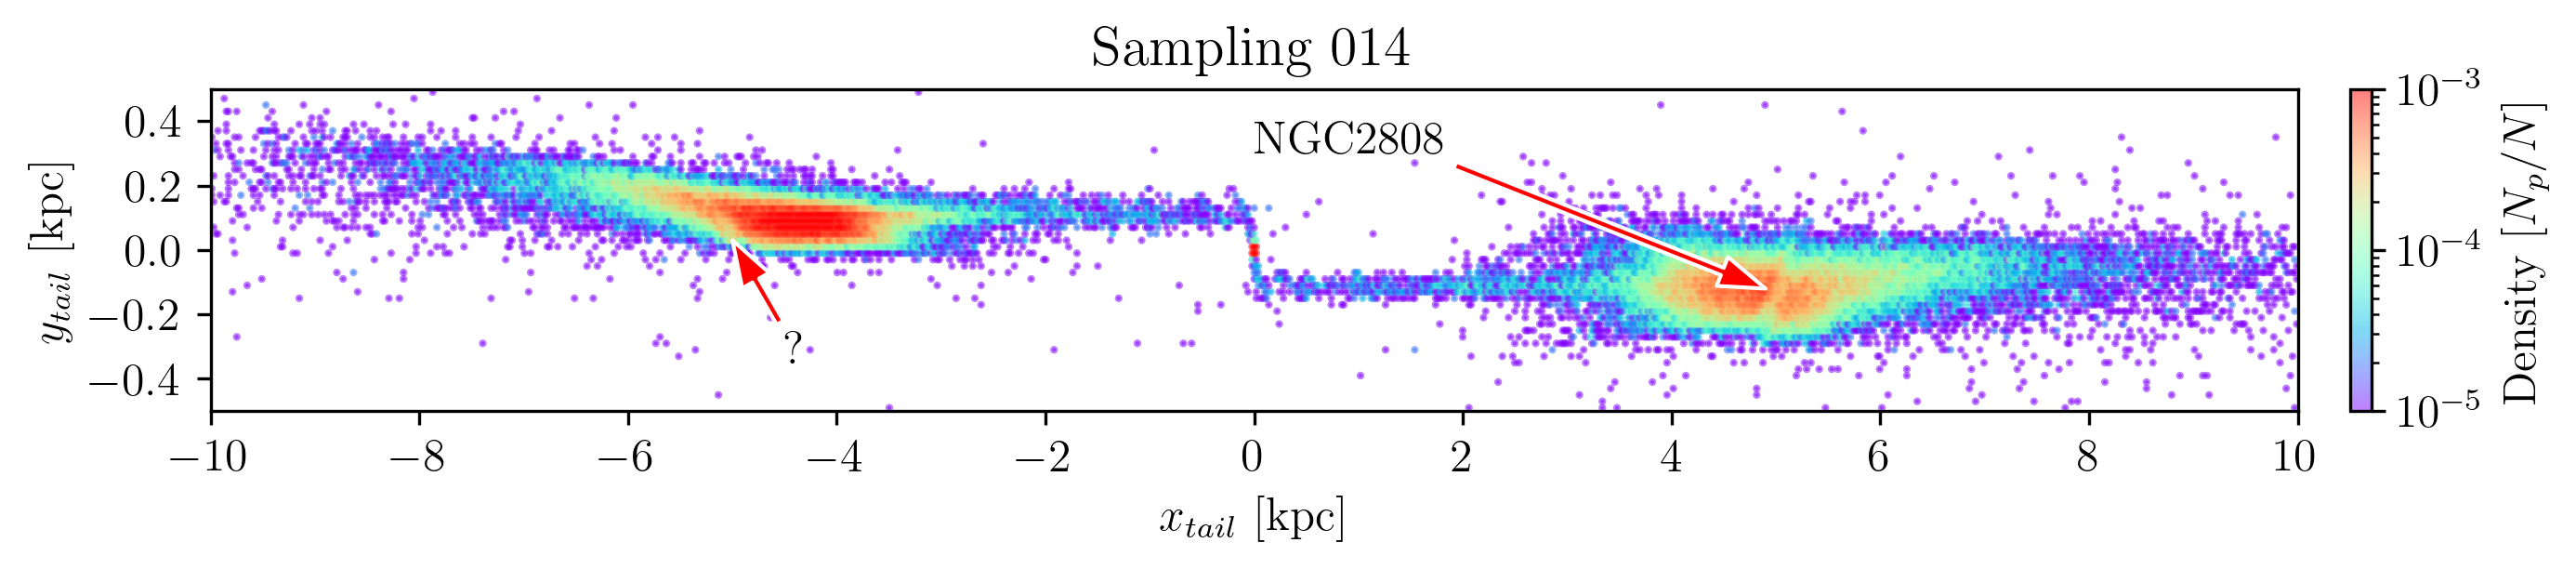
\includegraphics[width=\linewidth]{gallery_of_gaps_monte-carlo-014.png}
      \caption{Gap Gallery}
      \label{fig:TailCoordinates}
    \end{figure*}        


    \begin{figure*}
      \centering
      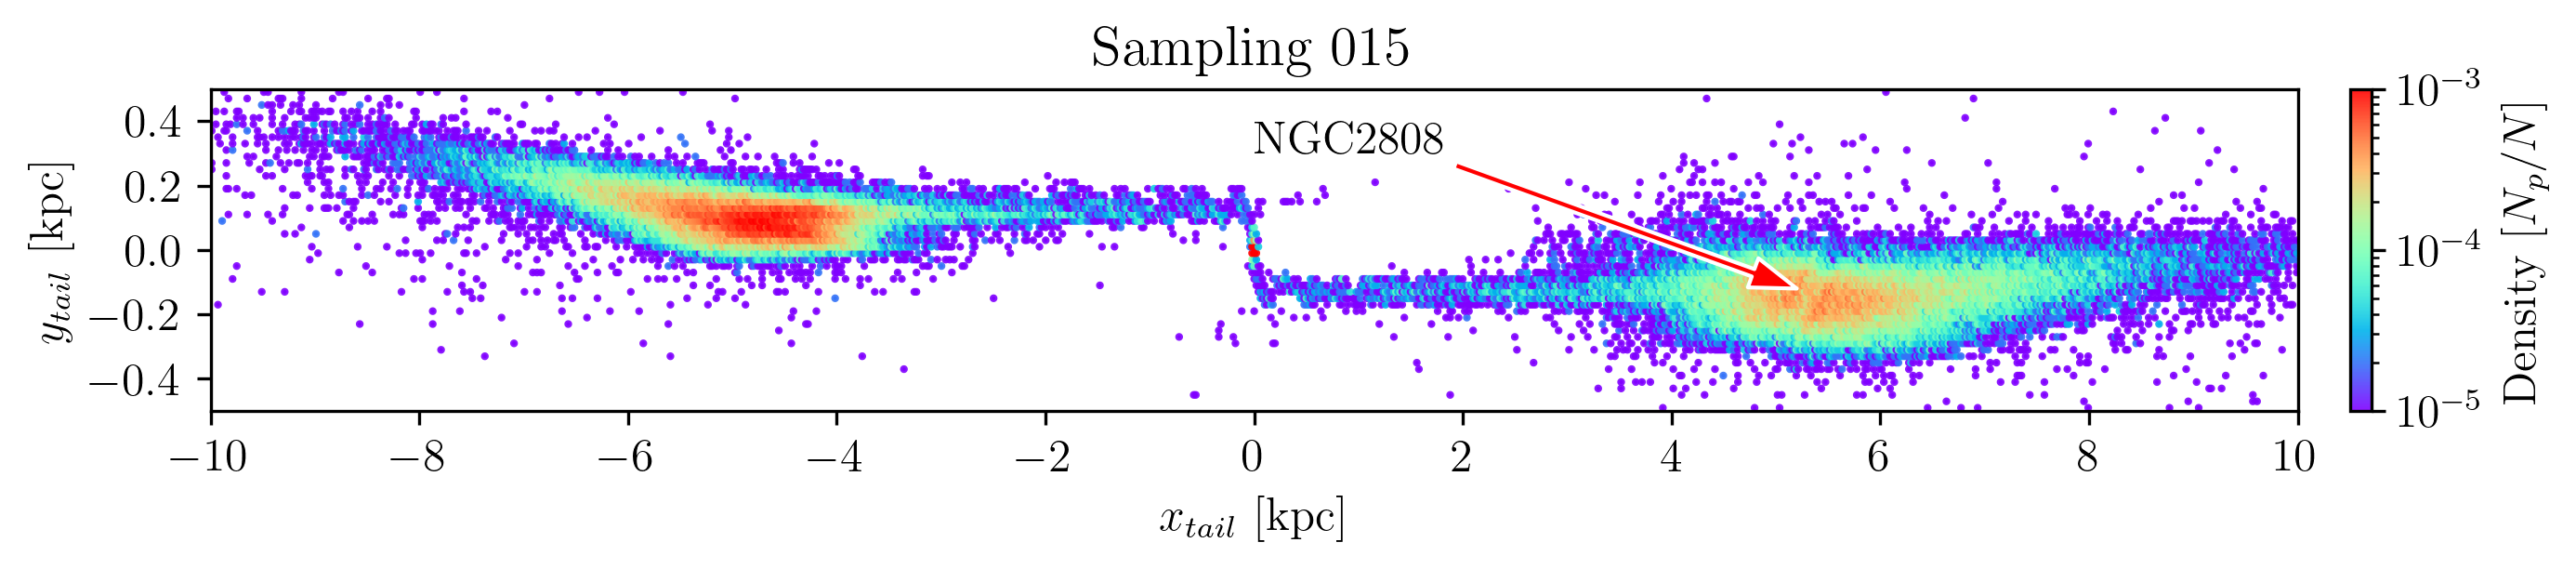
\includegraphics[width=\linewidth]{gallery_of_gaps_monte-carlo-015.png}
      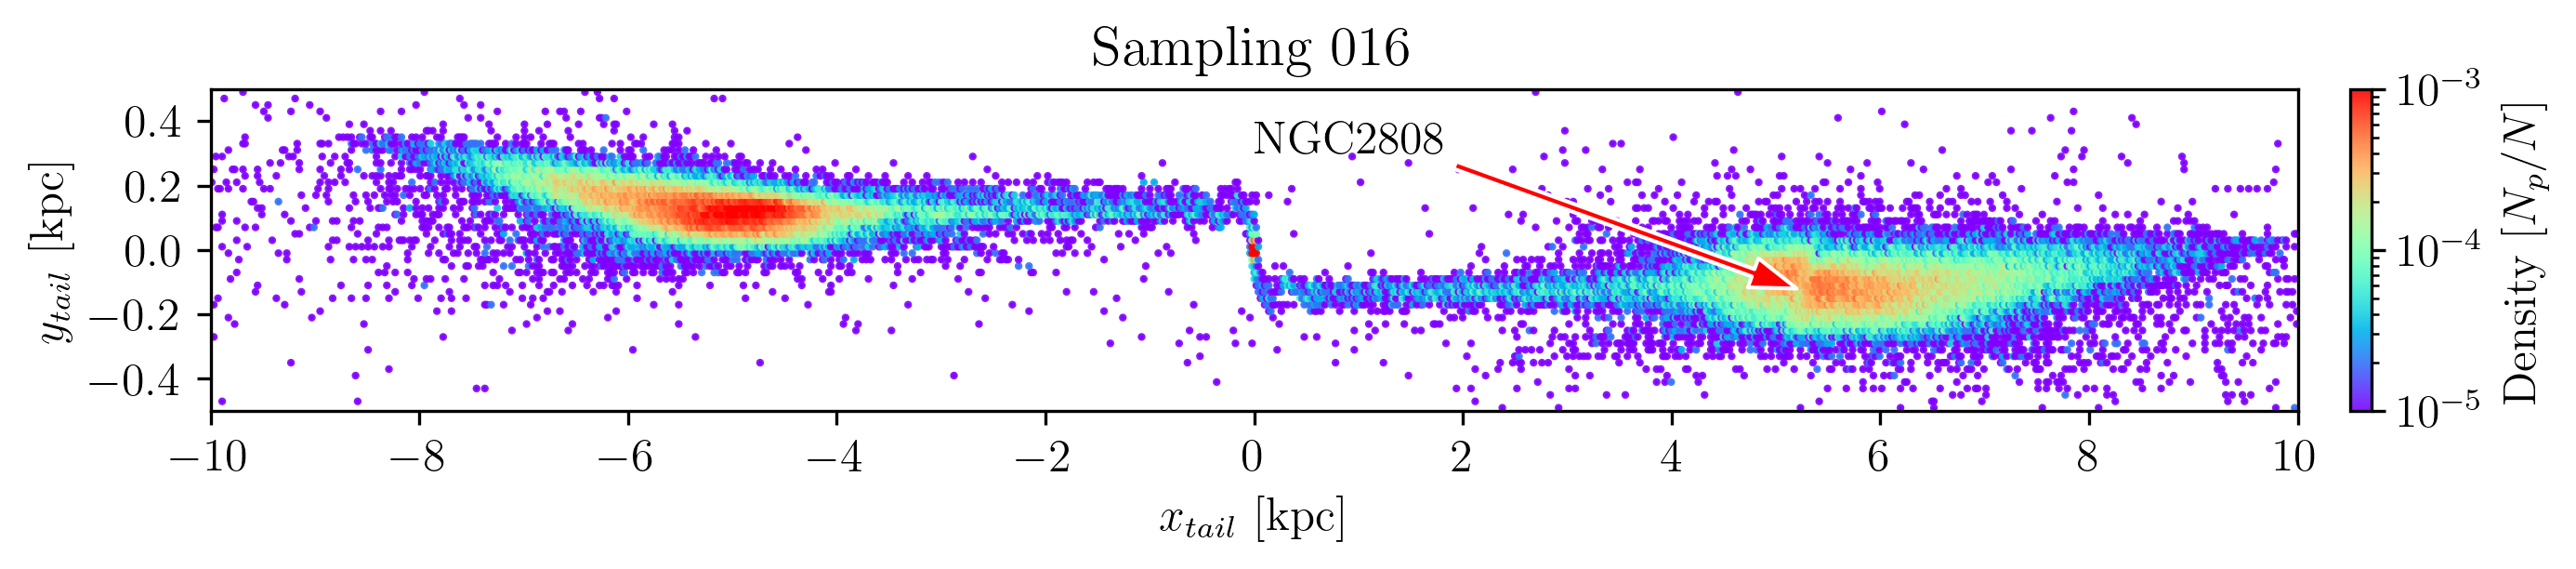
\includegraphics[width=\linewidth]{gallery_of_gaps_monte-carlo-016.png}
      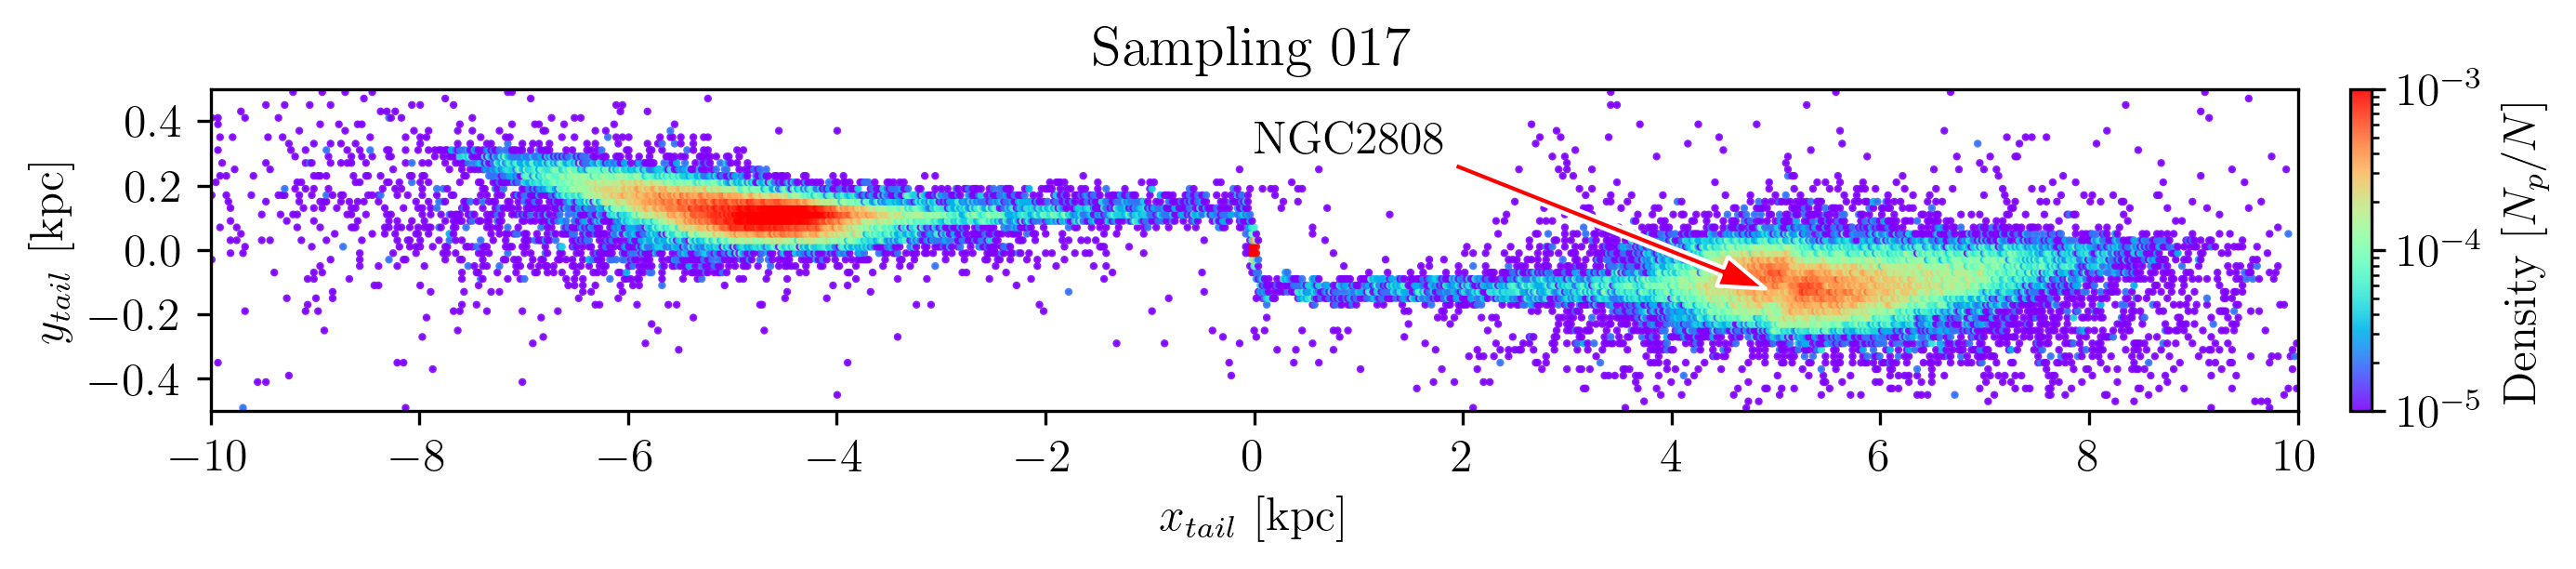
\includegraphics[width=\linewidth]{gallery_of_gaps_monte-carlo-017.png}
      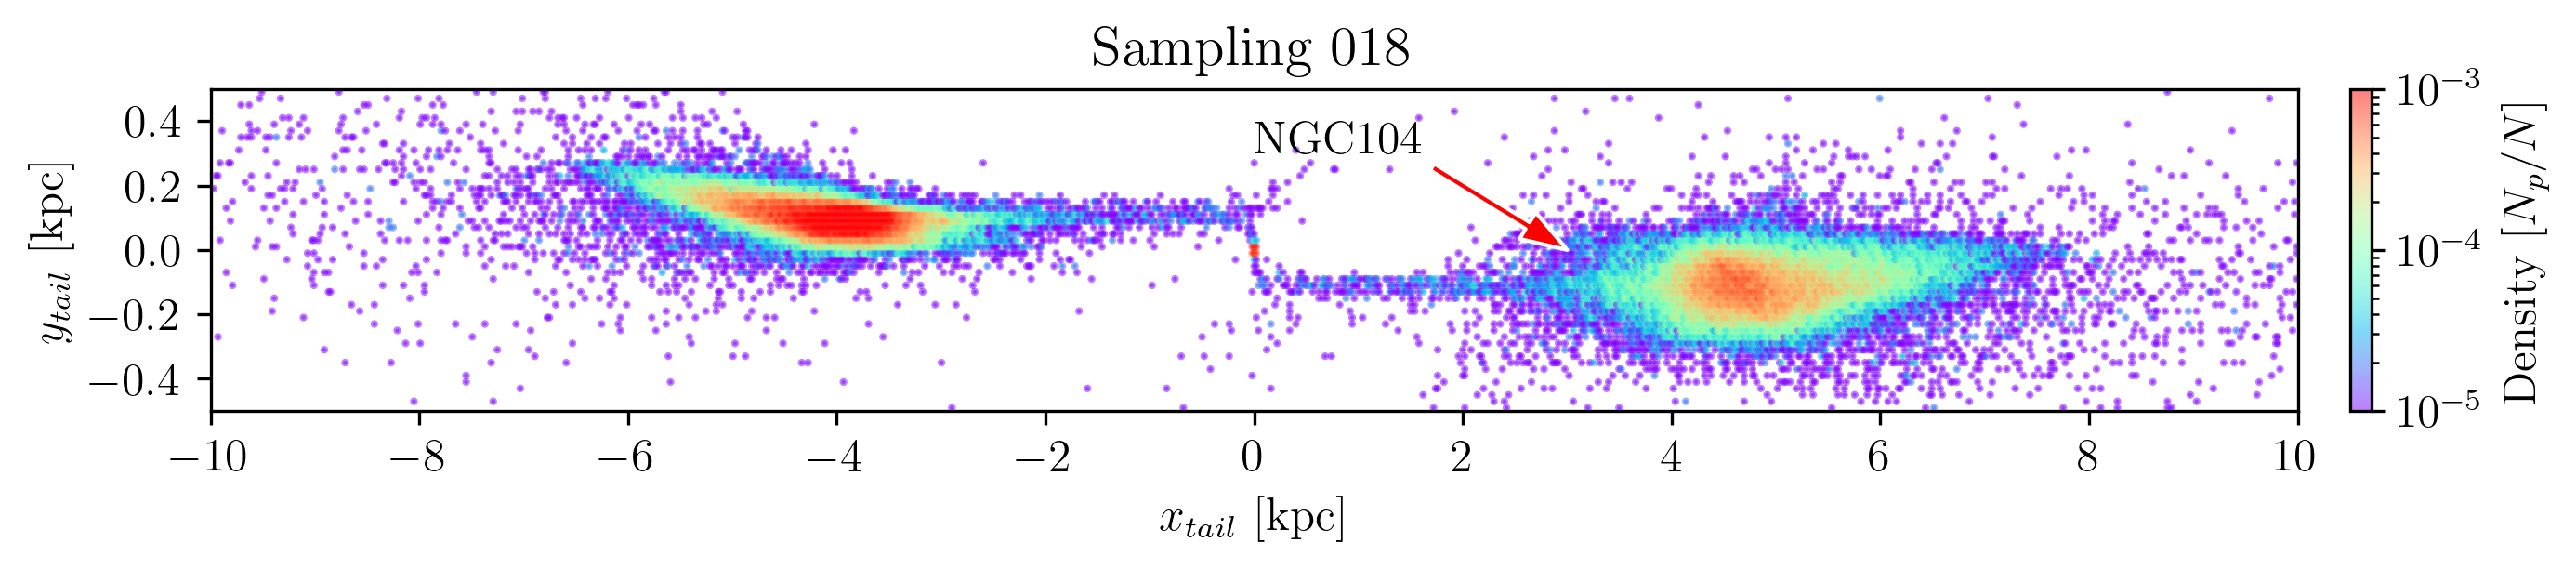
\includegraphics[width=\linewidth]{gallery_of_gaps_monte-carlo-018.png}
      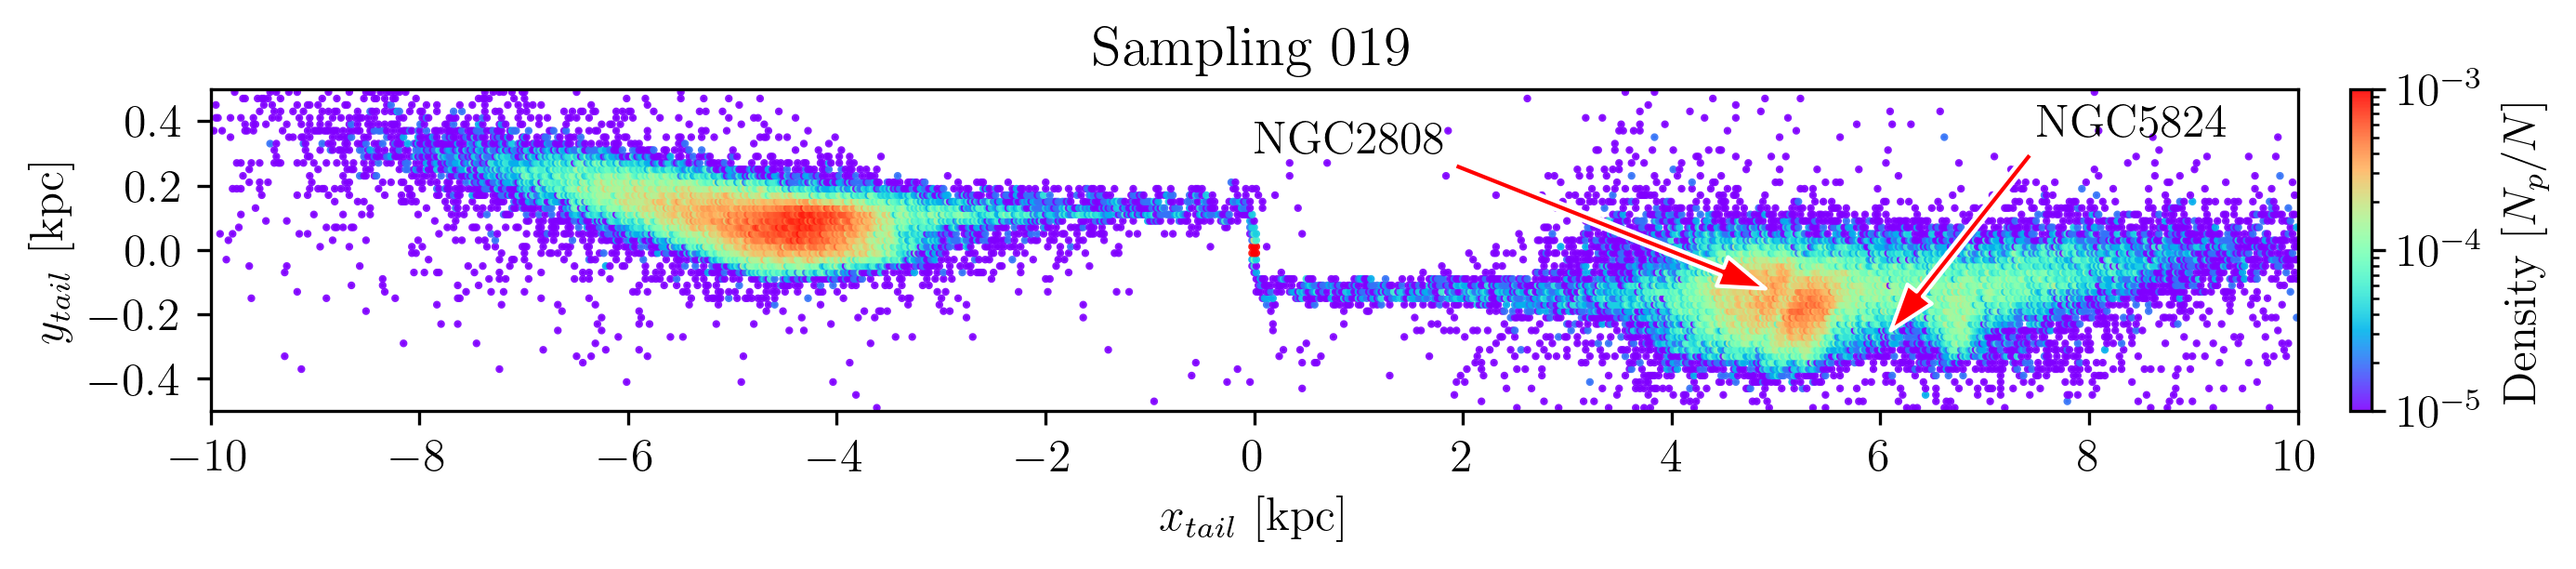
\includegraphics[width=\linewidth]{gallery_of_gaps_monte-carlo-019.png}
      \caption{Gap Gallery}
      \label{fig:TailCoordinates}
    \end{figure*}        

    \begin{figure*}
      \centering
      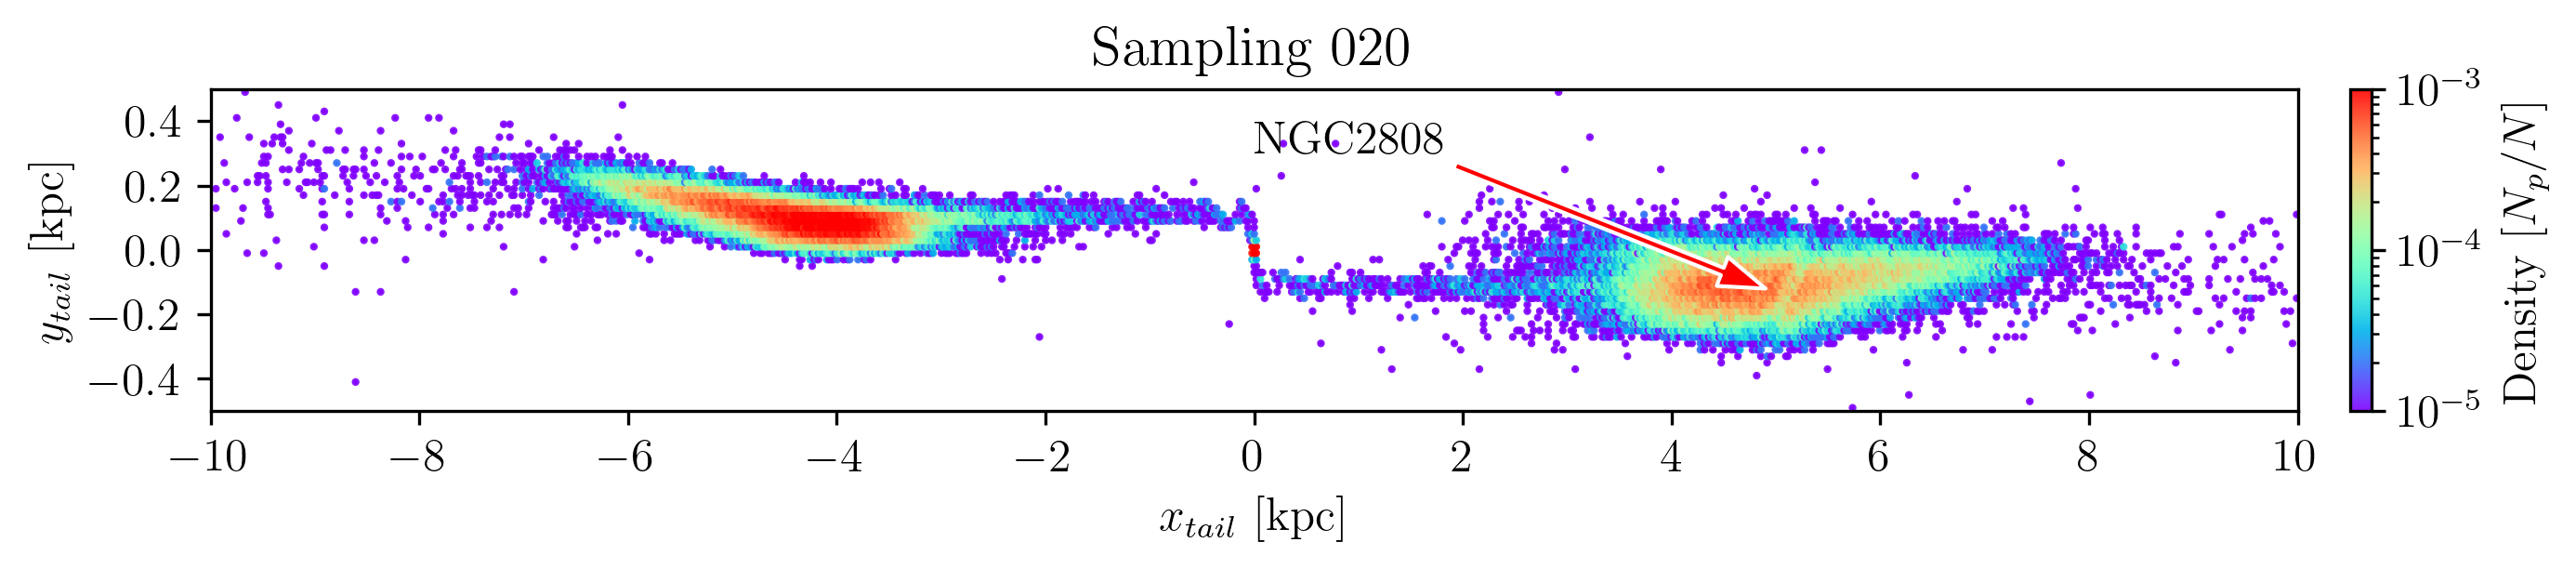
\includegraphics[width=\linewidth]{gallery_of_gaps_monte-carlo-020.png}
      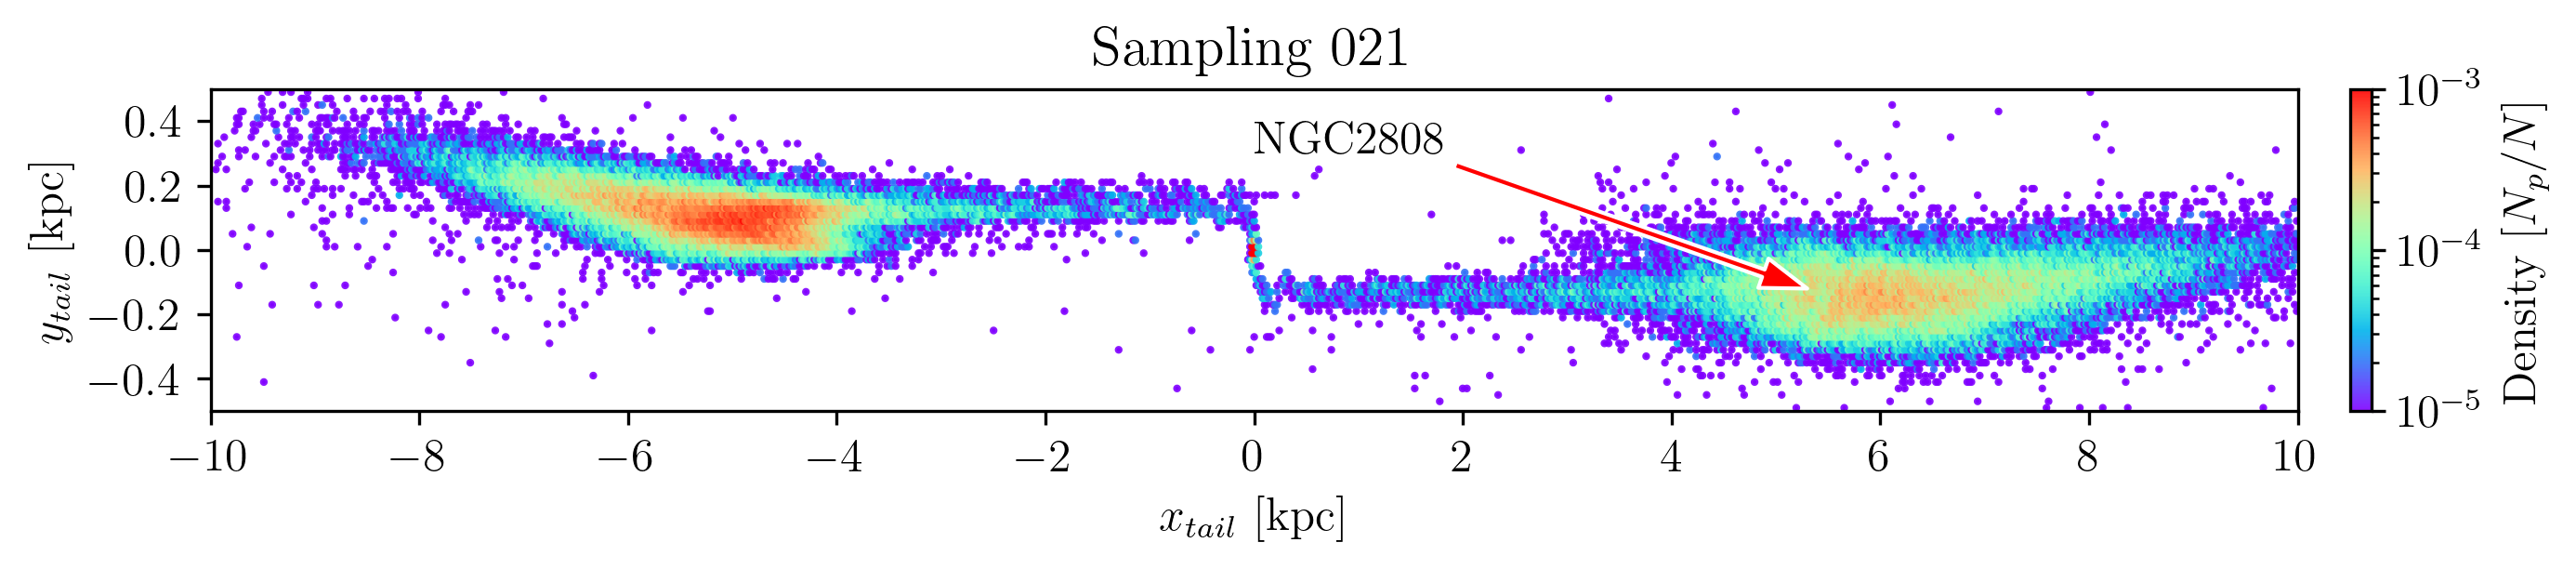
\includegraphics[width=\linewidth]{gallery_of_gaps_monte-carlo-021.png}
      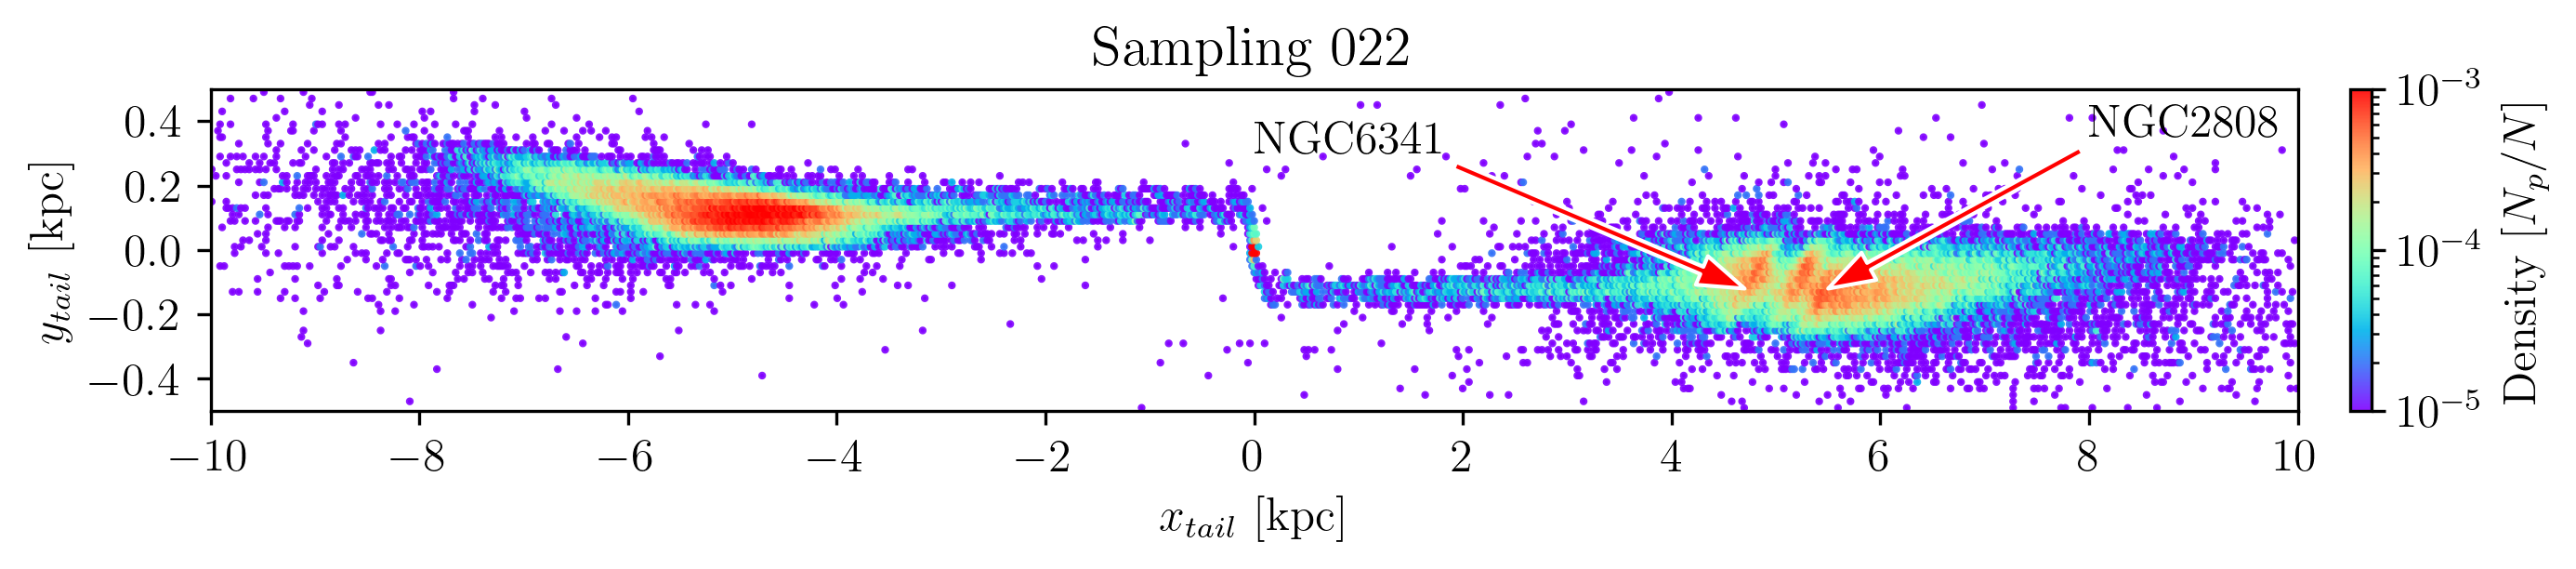
\includegraphics[width=\linewidth]{gallery_of_gaps_monte-carlo-022.png}
      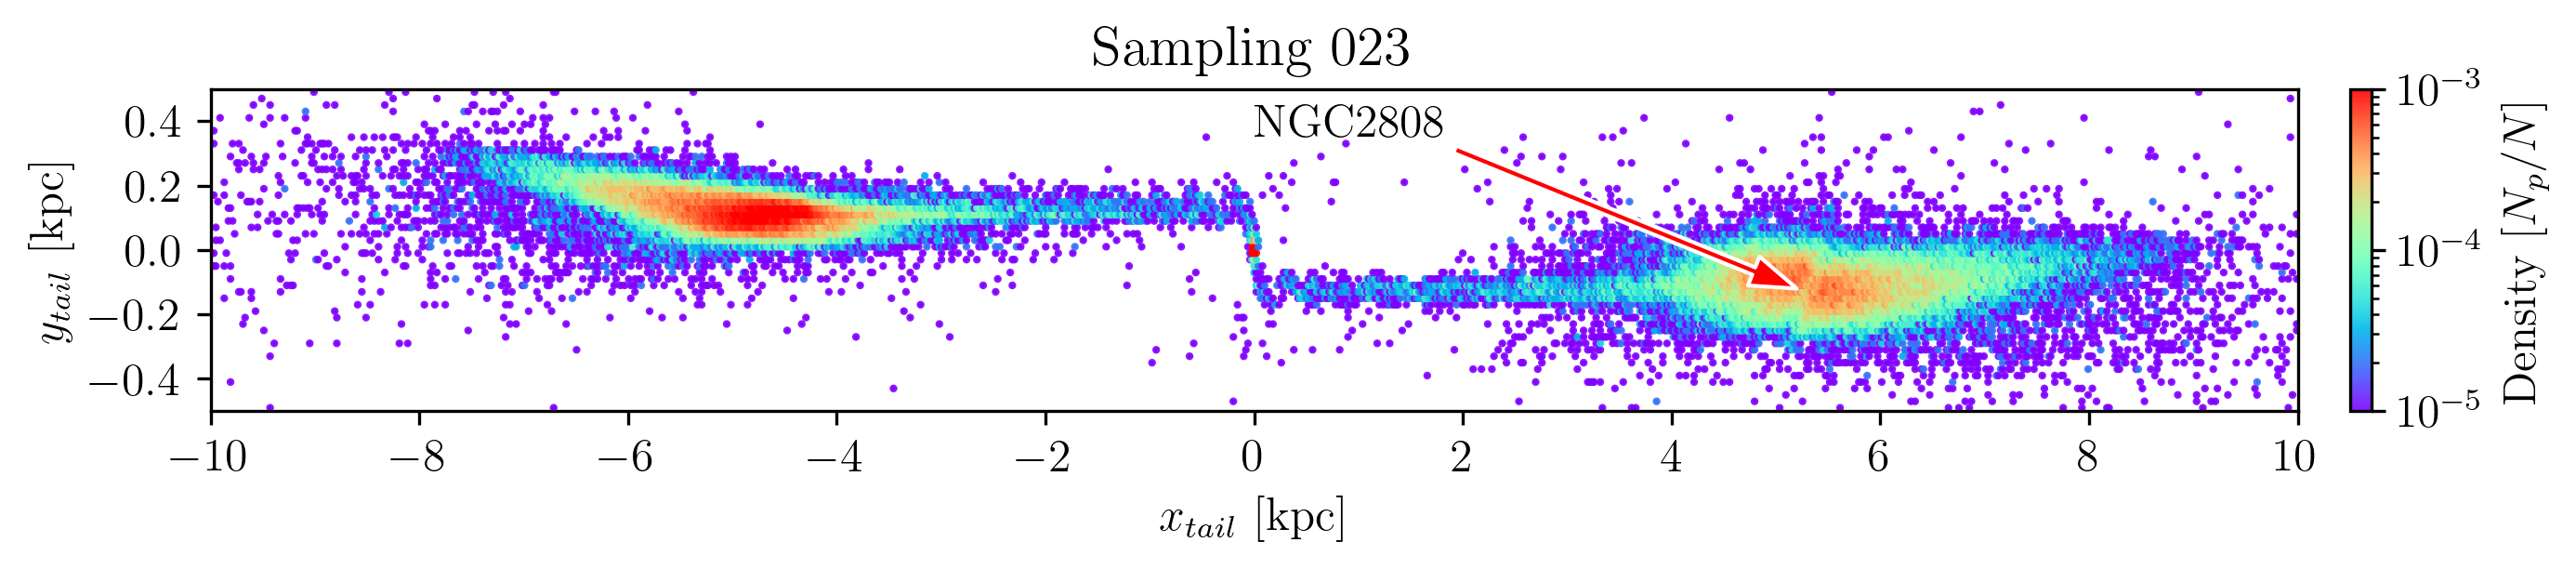
\includegraphics[width=\linewidth]{gallery_of_gaps_monte-carlo-023.png}
      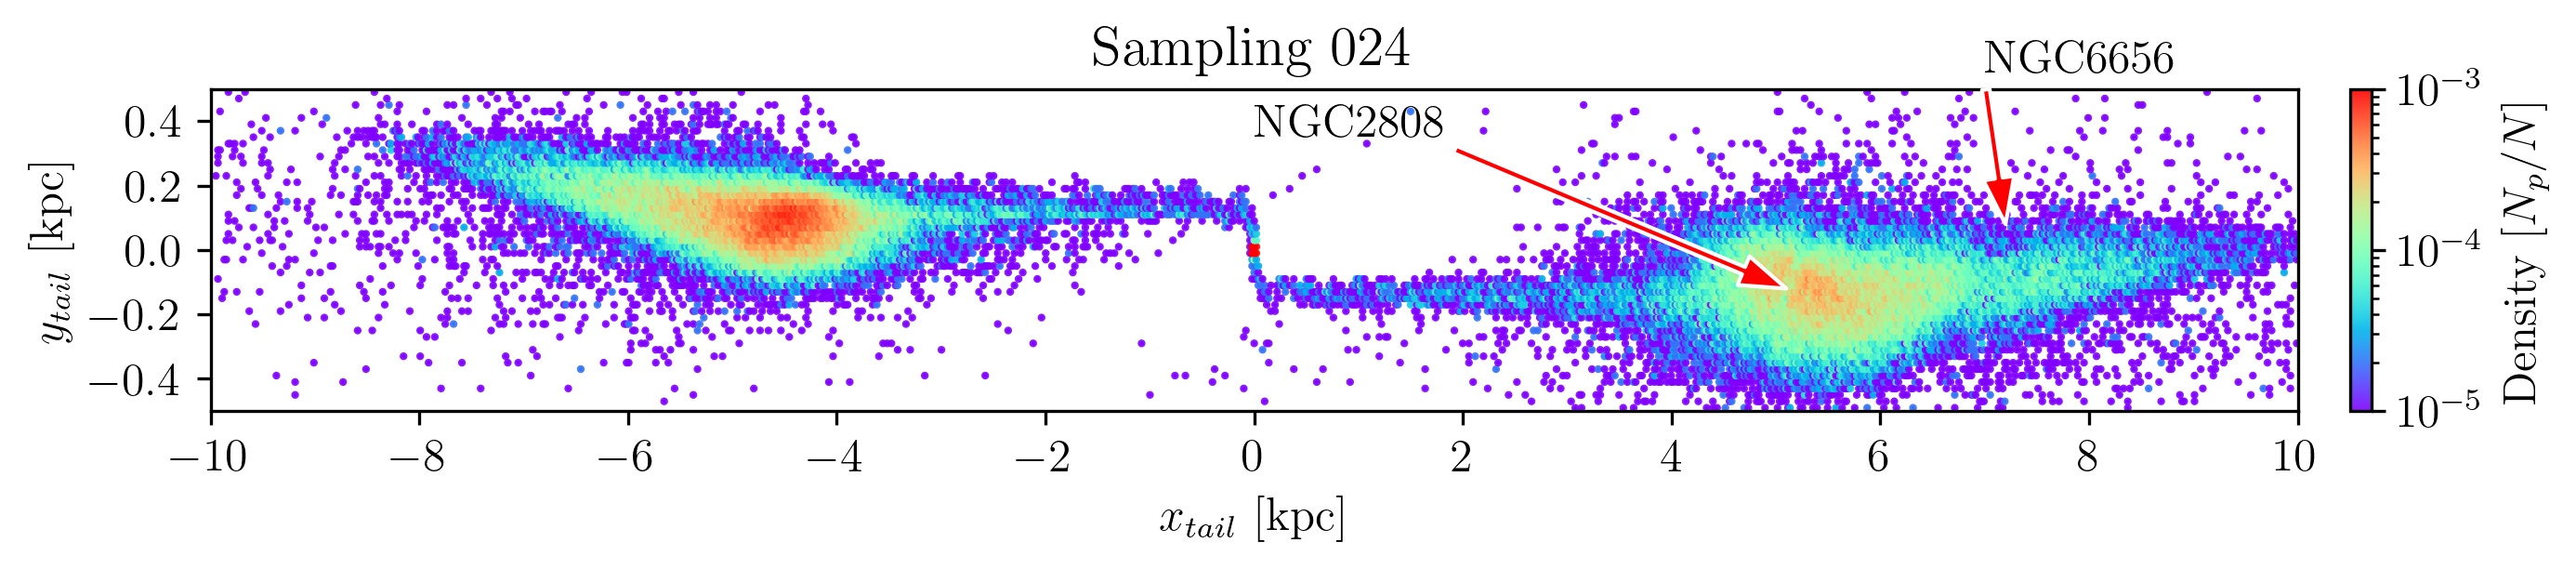
\includegraphics[width=\linewidth]{gallery_of_gaps_monte-carlo-024.png}
      \caption{Gap Gallery}
      \label{fig:TailCoordinates}
    \end{figure*}        

    \begin{figure*}
      \centering
      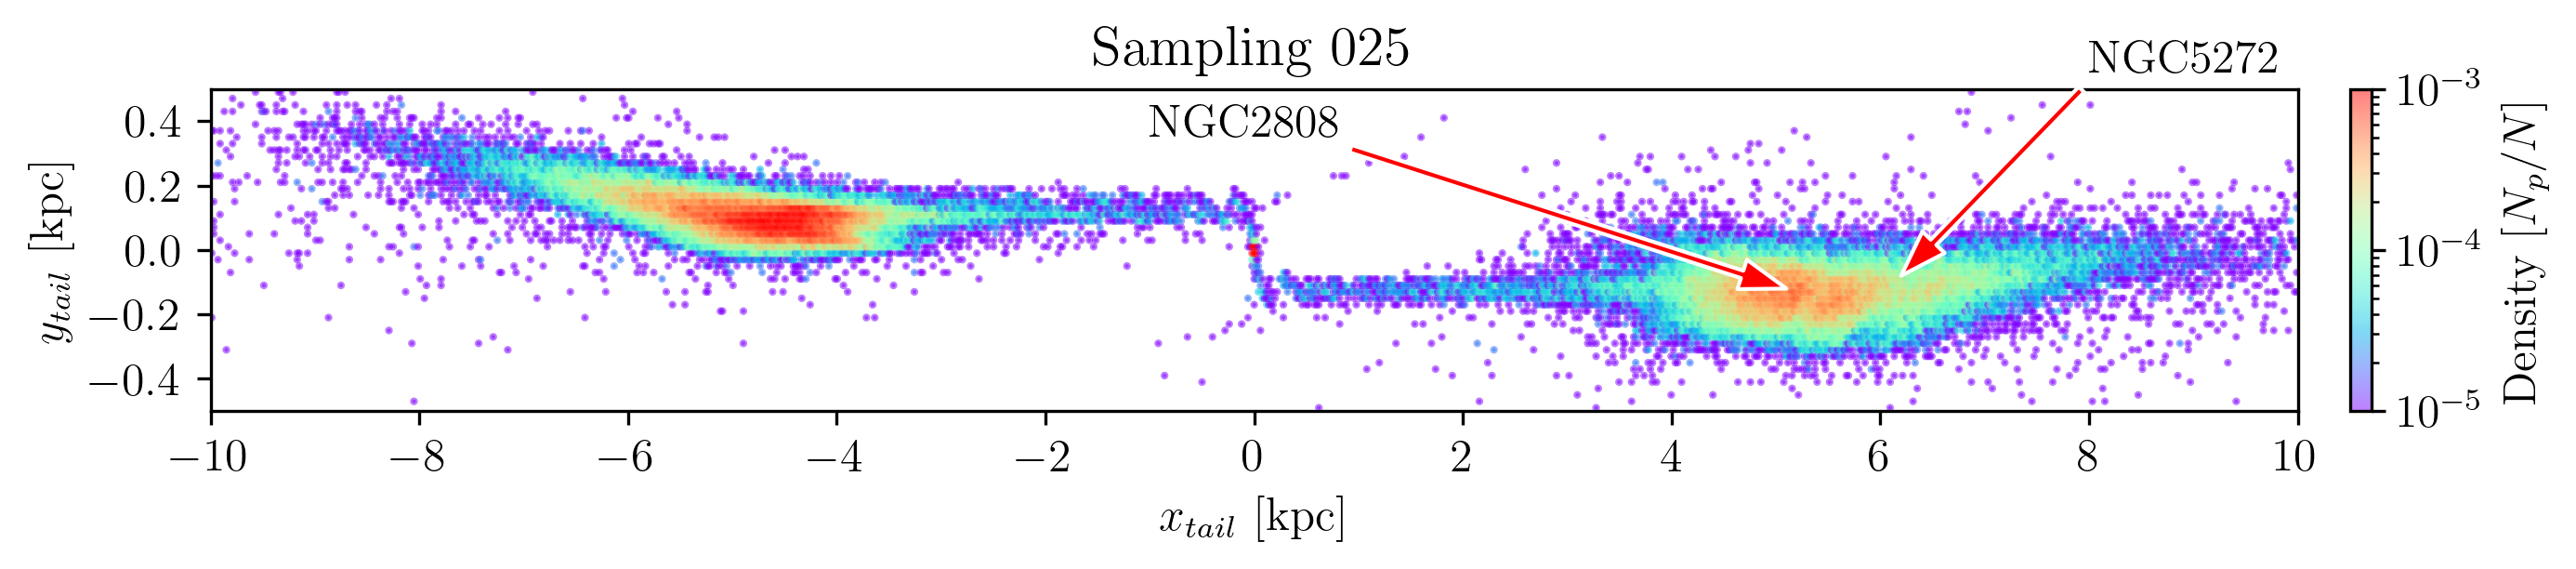
\includegraphics[width=\linewidth]{gallery_of_gaps_monte-carlo-025.png}
      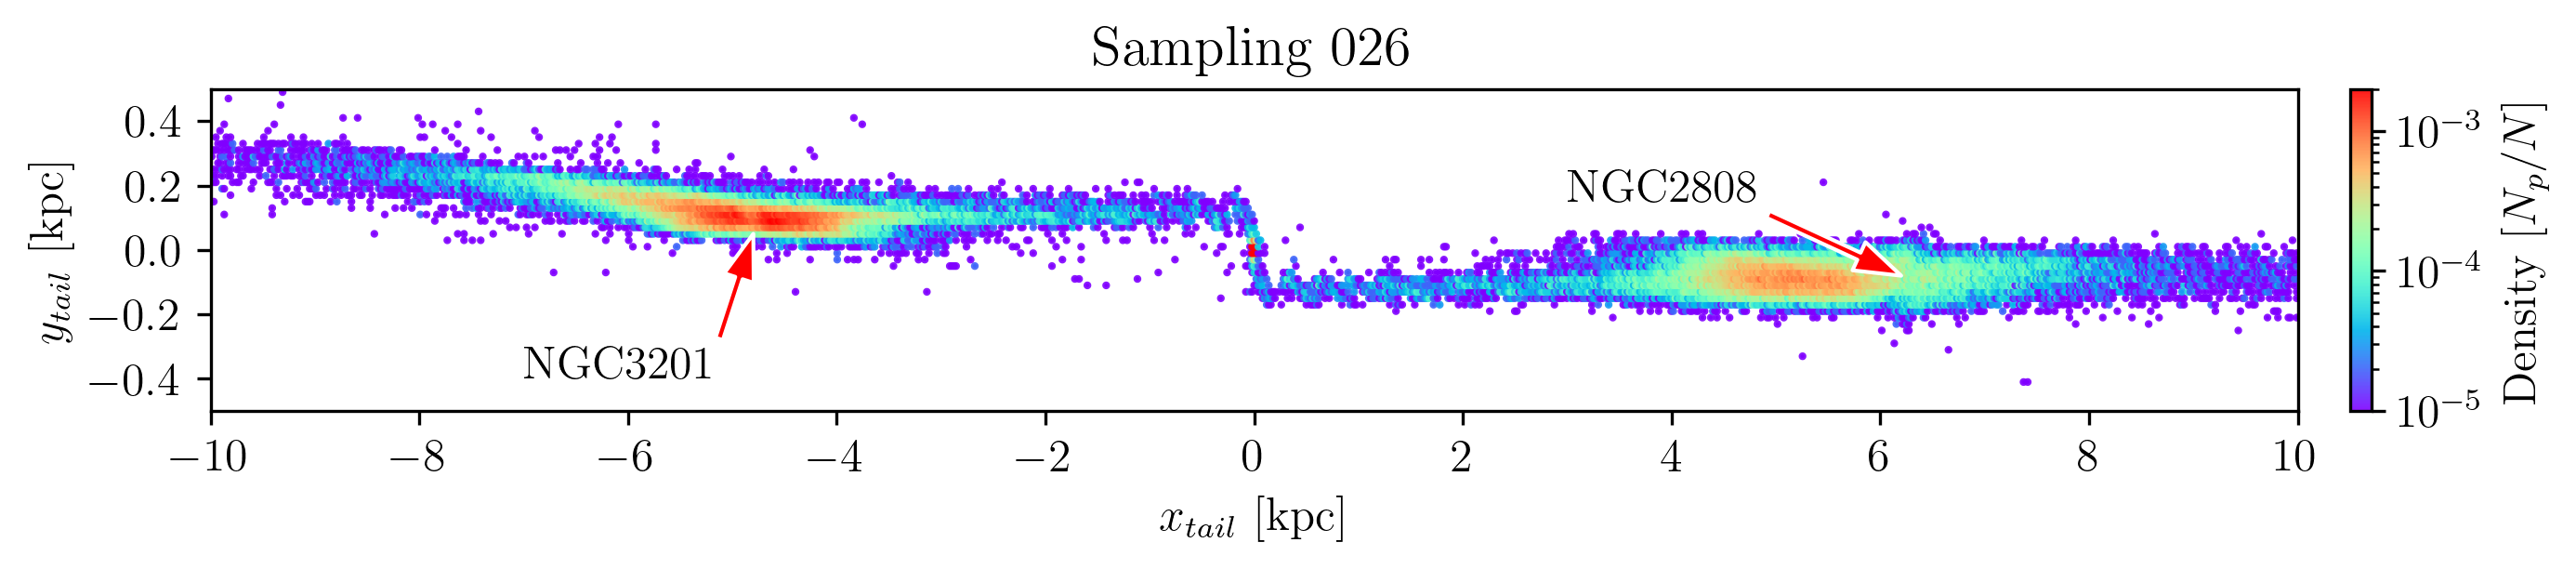
\includegraphics[width=\linewidth]{gallery_of_gaps_monte-carlo-026.png}
      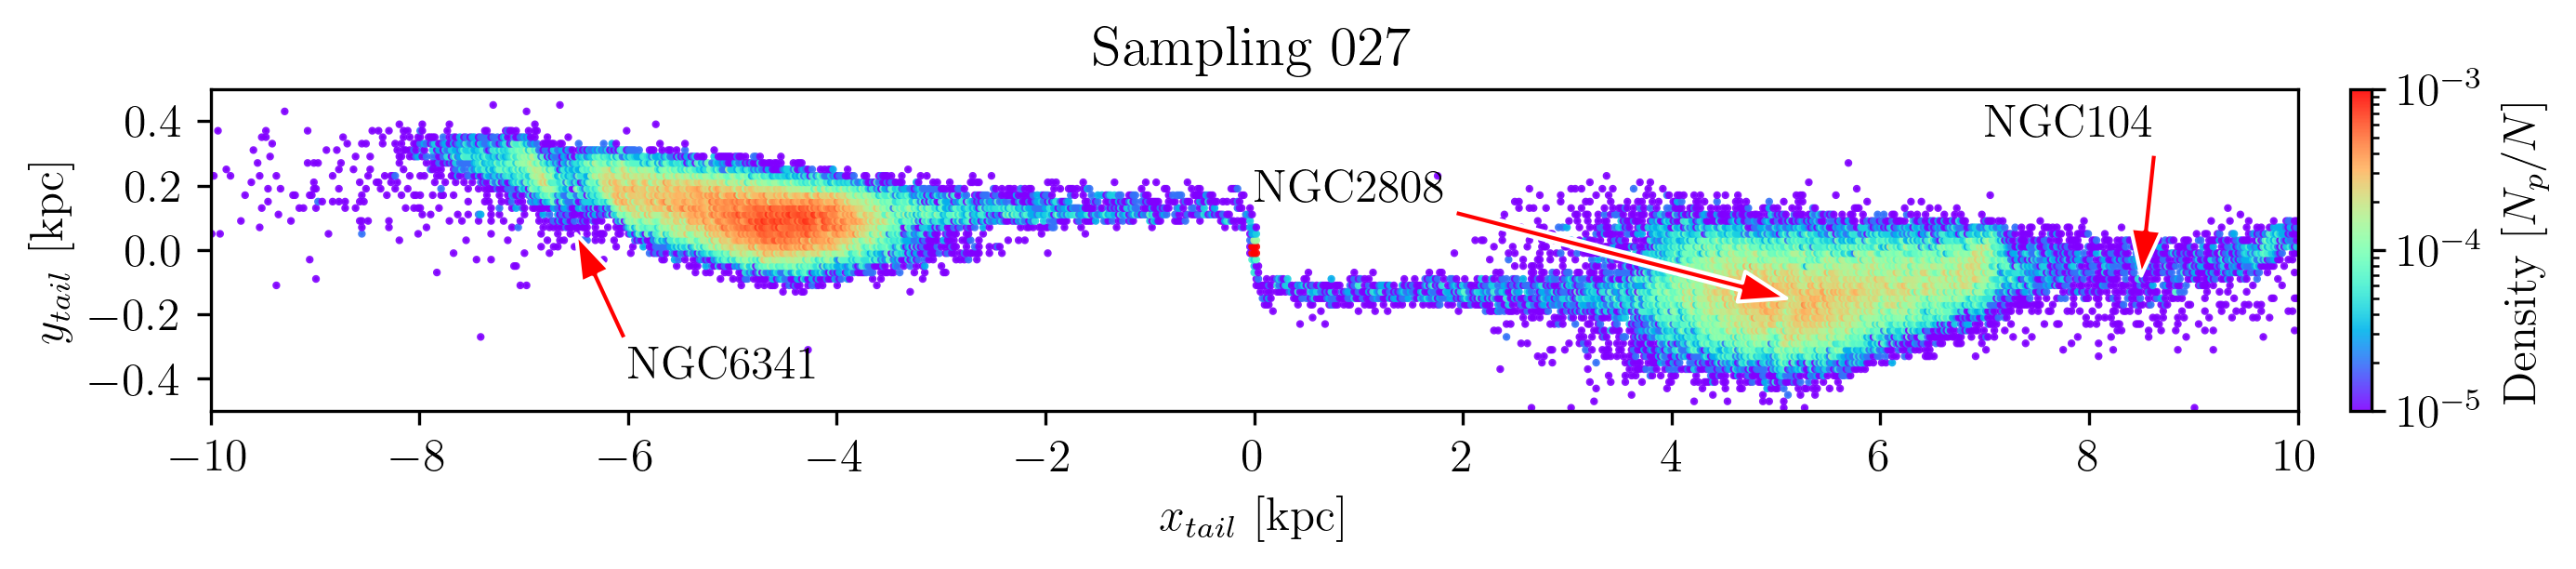
\includegraphics[width=\linewidth]{gallery_of_gaps_monte-carlo-027.png}
      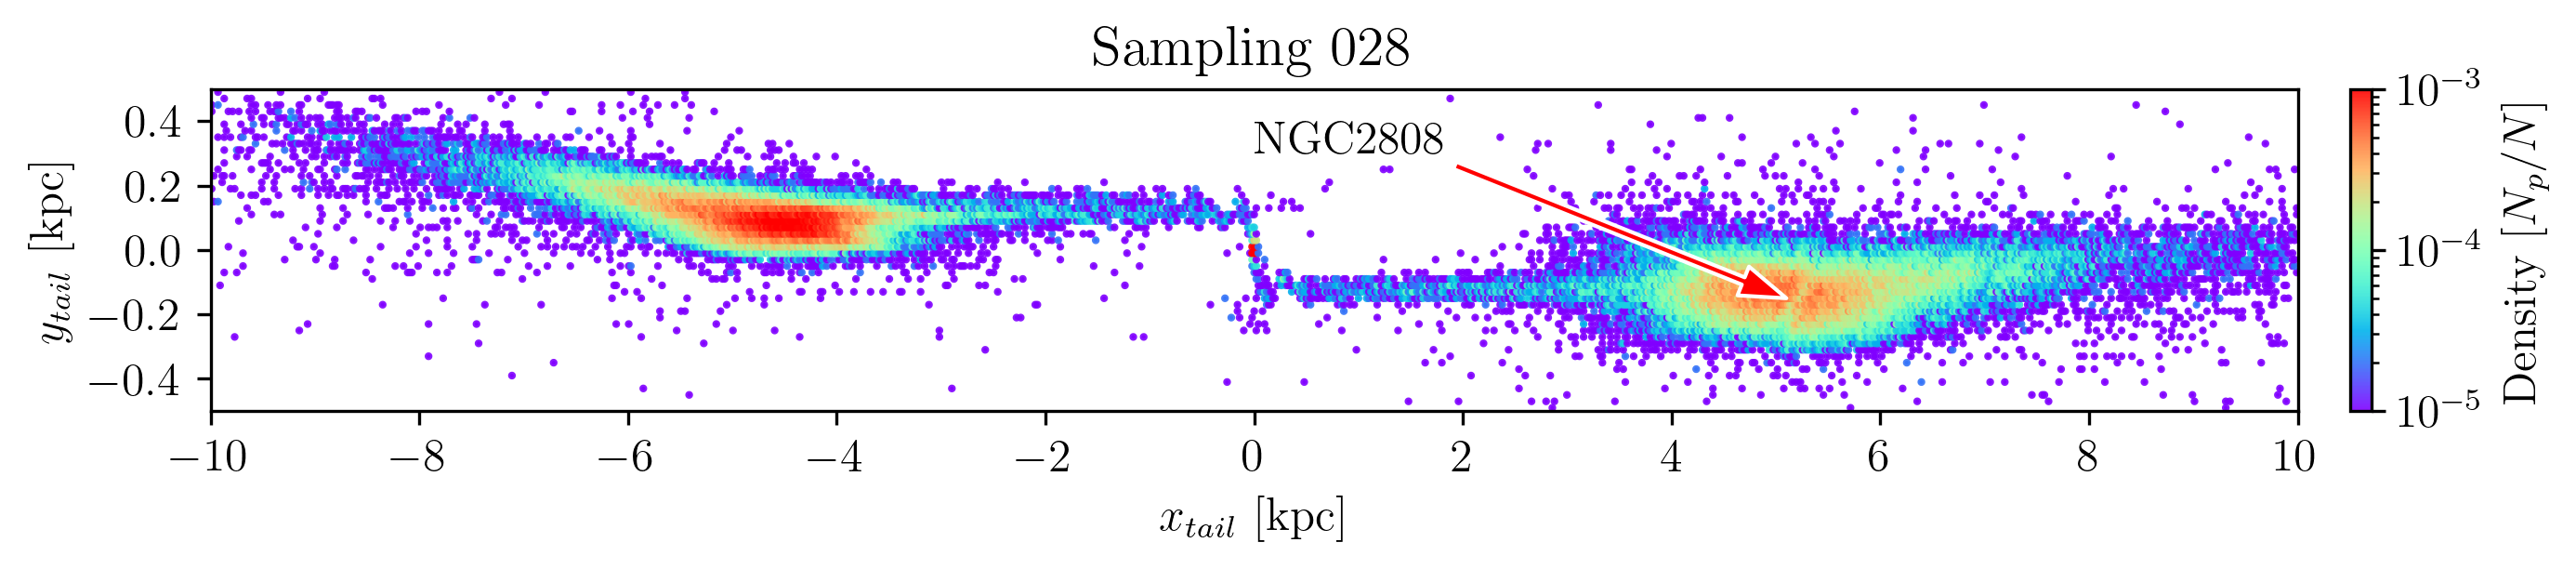
\includegraphics[width=\linewidth]{gallery_of_gaps_monte-carlo-028.png}
      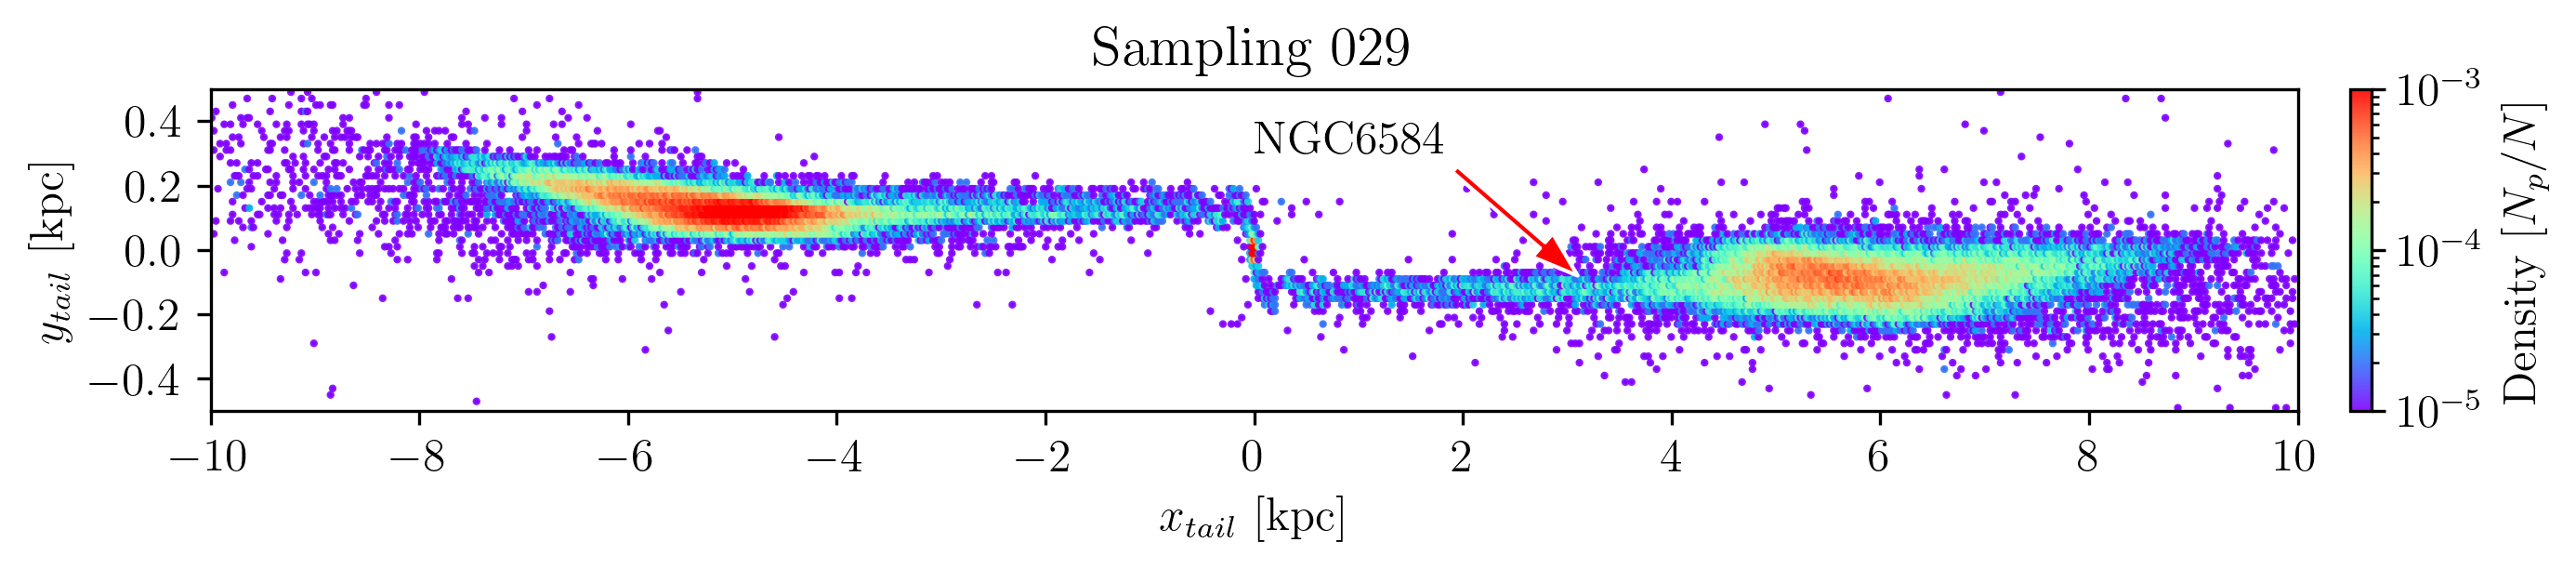
\includegraphics[width=\linewidth]{gallery_of_gaps_monte-carlo-029.png}
      \caption{Gap Gallery}
      \label{fig:TailCoordinates}
    \end{figure*}        

    \begin{figure*}
      \centering
      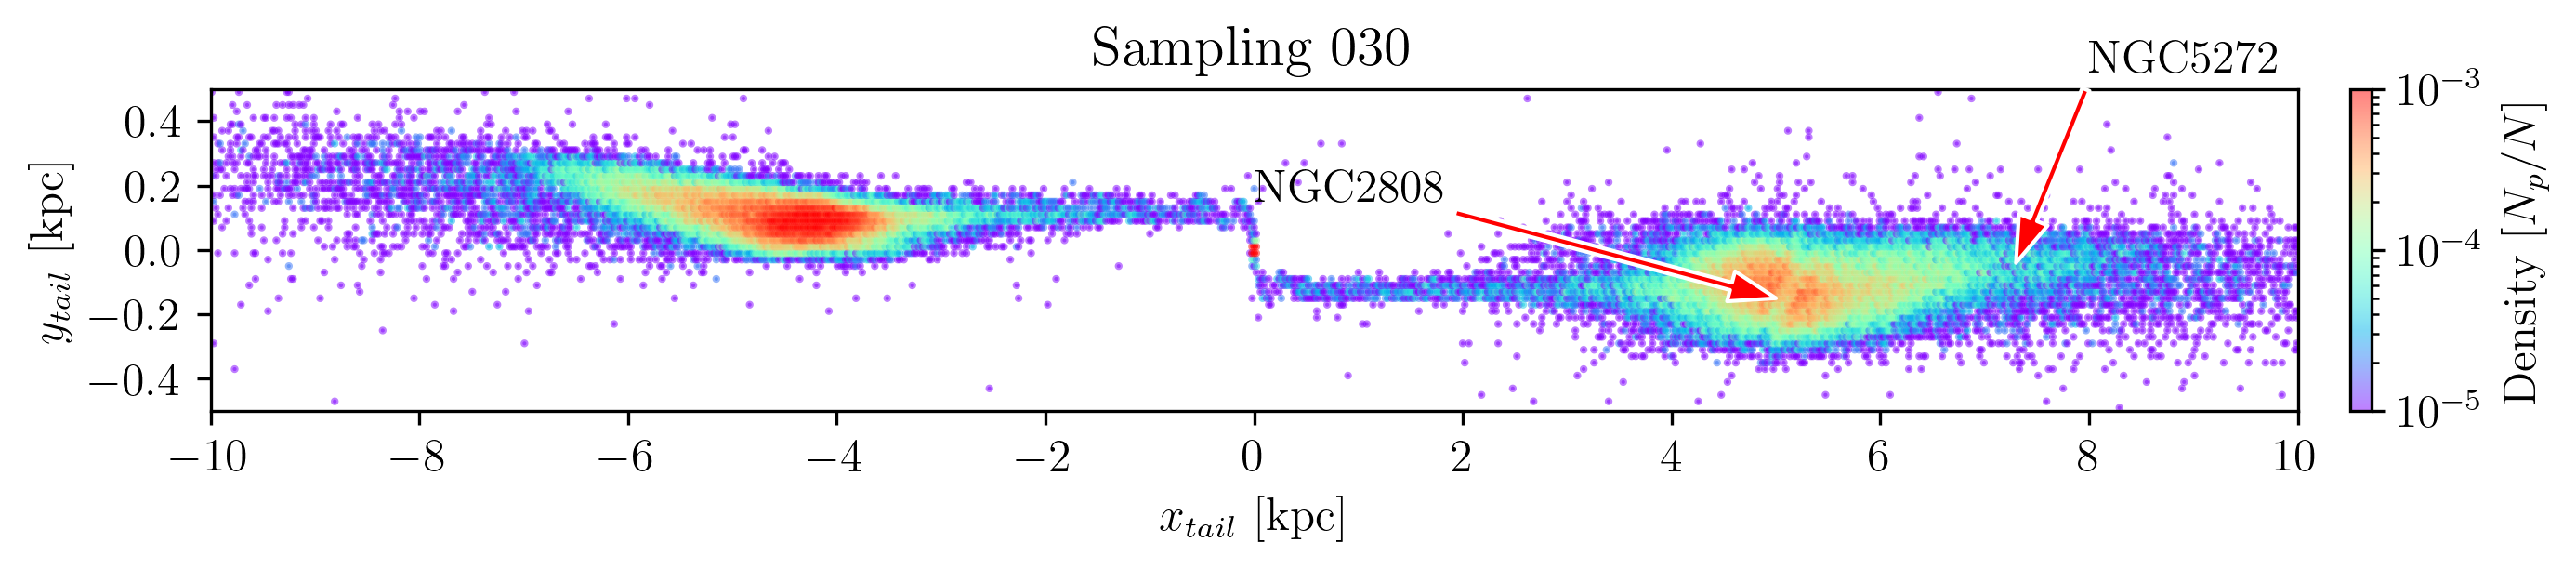
\includegraphics[width=\linewidth]{gallery_of_gaps_monte-carlo-030.png}
      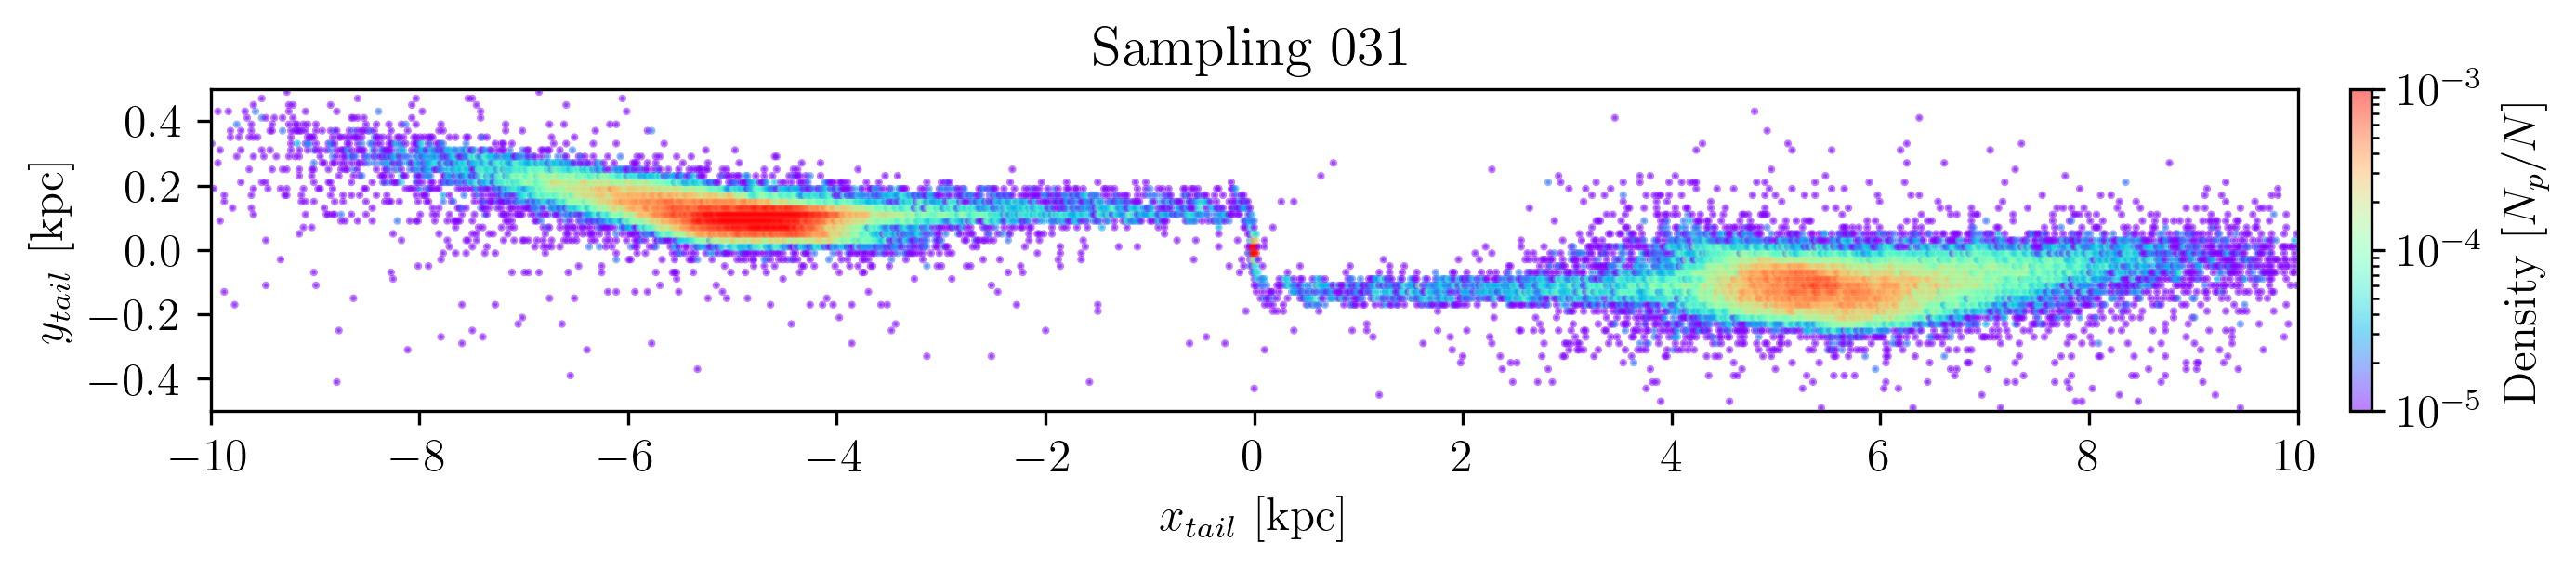
\includegraphics[width=\linewidth]{gallery_of_gaps_monte-carlo-031.png}
      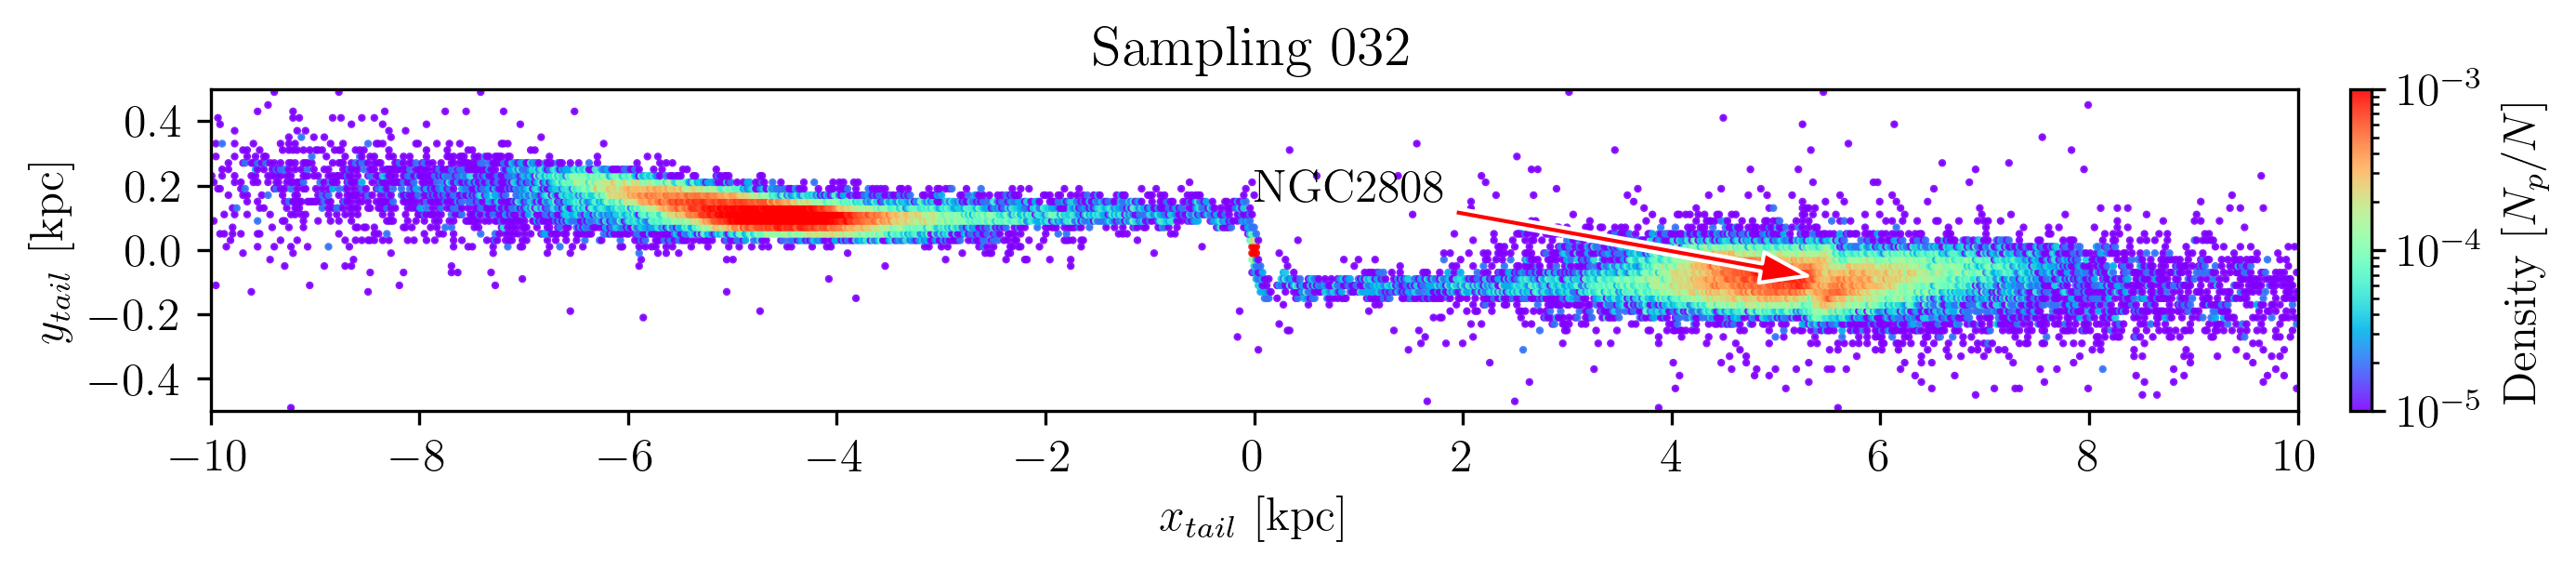
\includegraphics[width=\linewidth]{gallery_of_gaps_monte-carlo-032.png}
      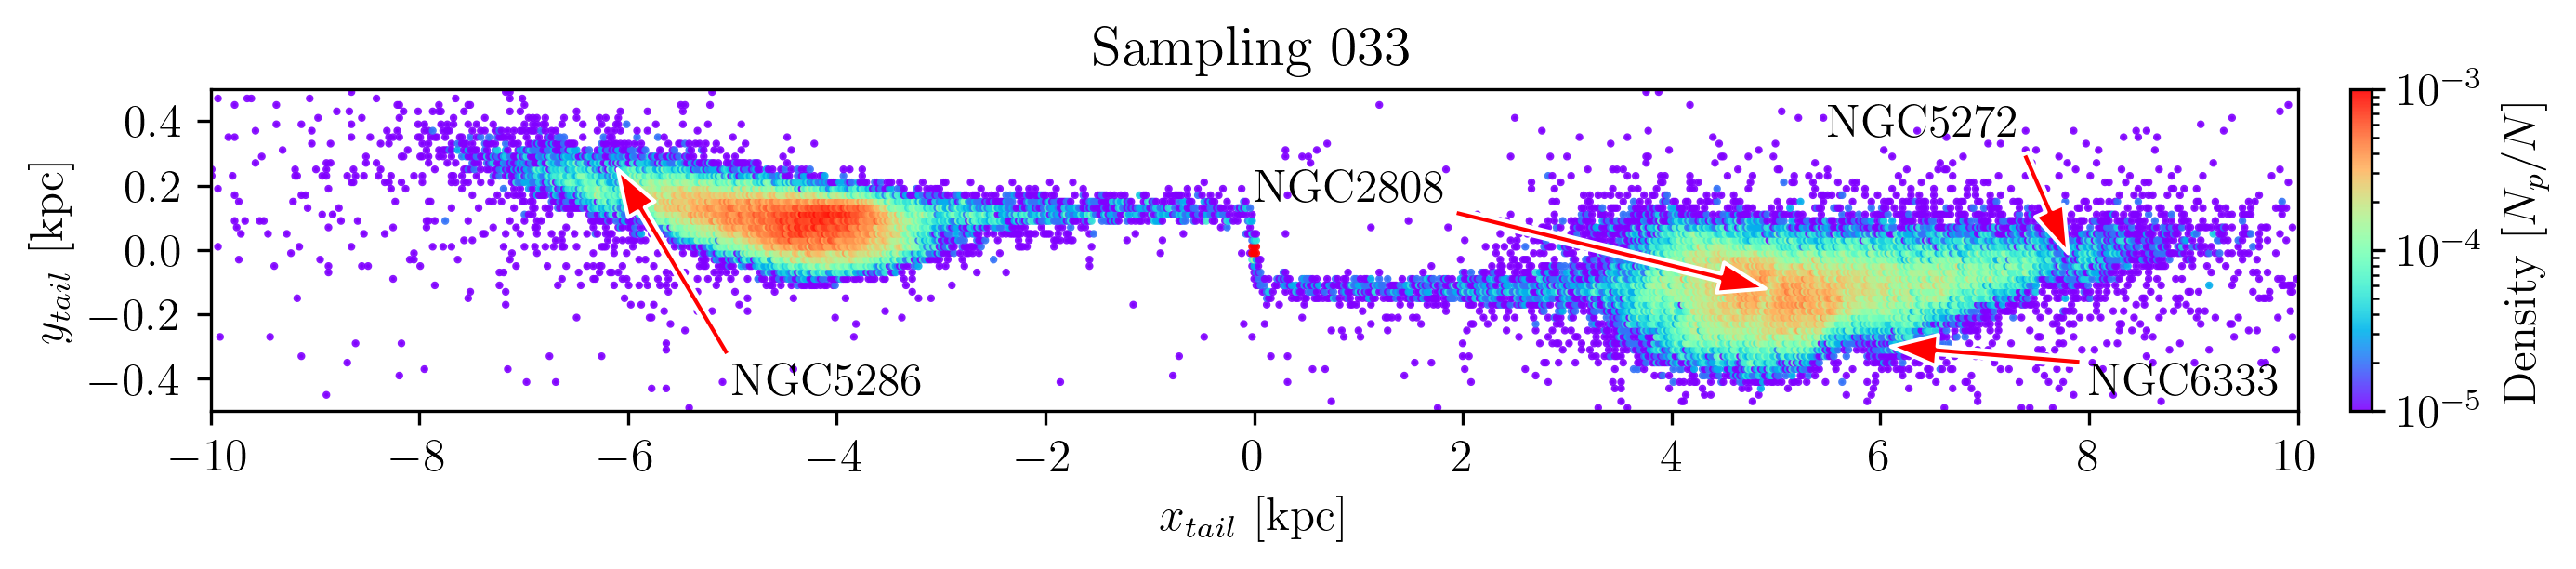
\includegraphics[width=\linewidth]{gallery_of_gaps_monte-carlo-033.png}
      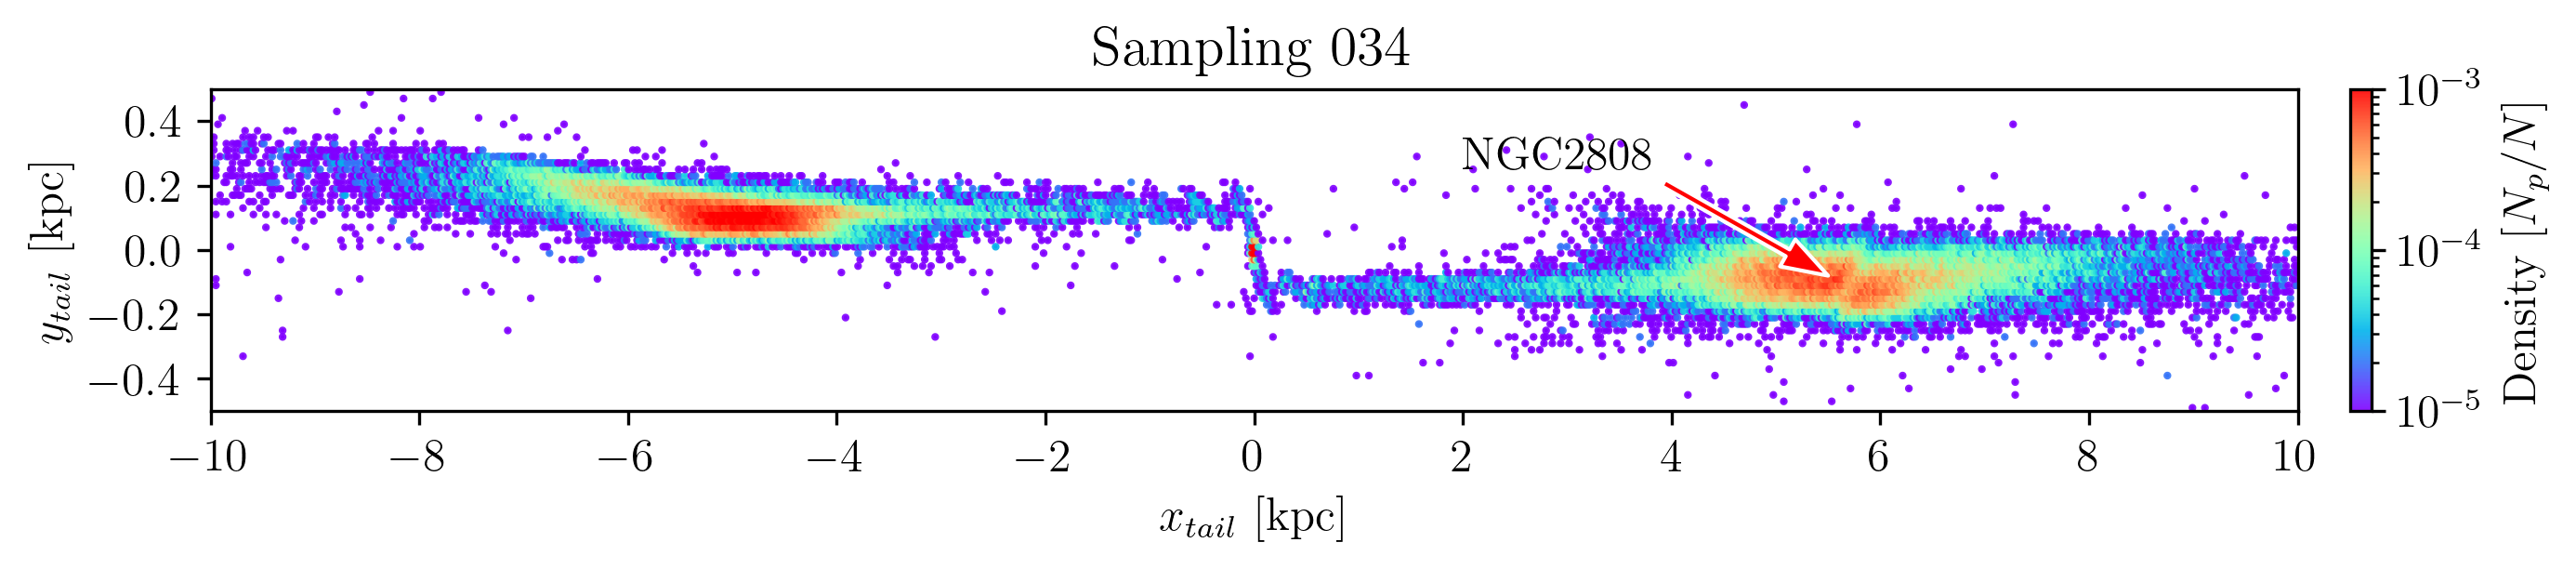
\includegraphics[width=\linewidth]{gallery_of_gaps_monte-carlo-034.png}
      \caption{Gap Gallery}
      \label{fig:TailCoordinates}
    \end{figure*}        

    \begin{figure*}
      \centering
      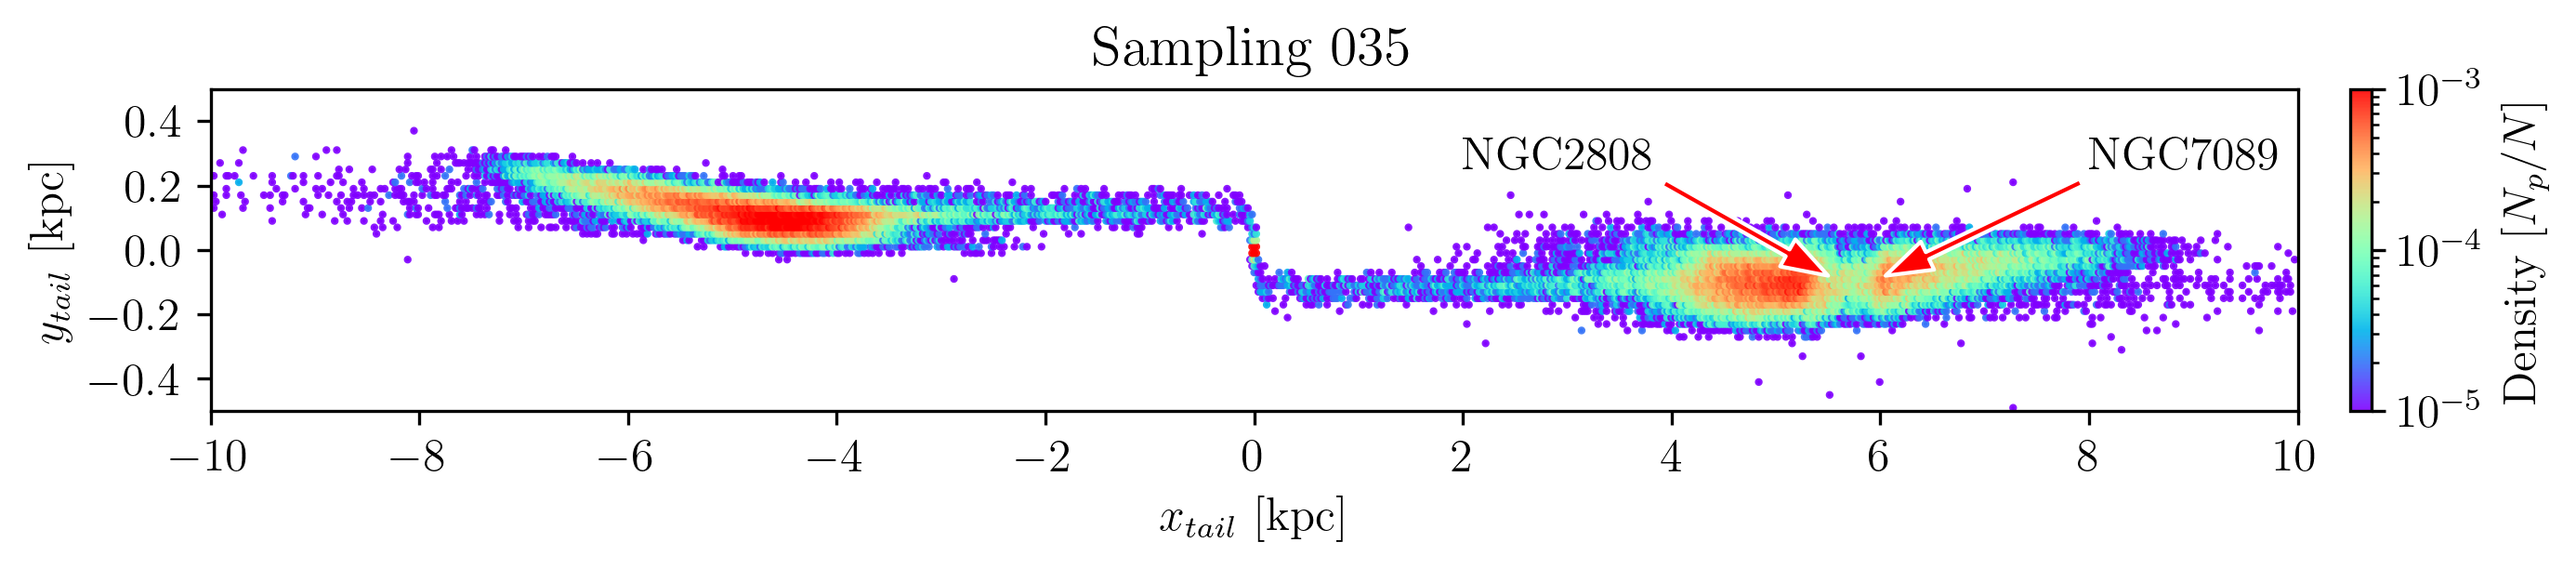
\includegraphics[width=\linewidth]{gallery_of_gaps_monte-carlo-035.png}
      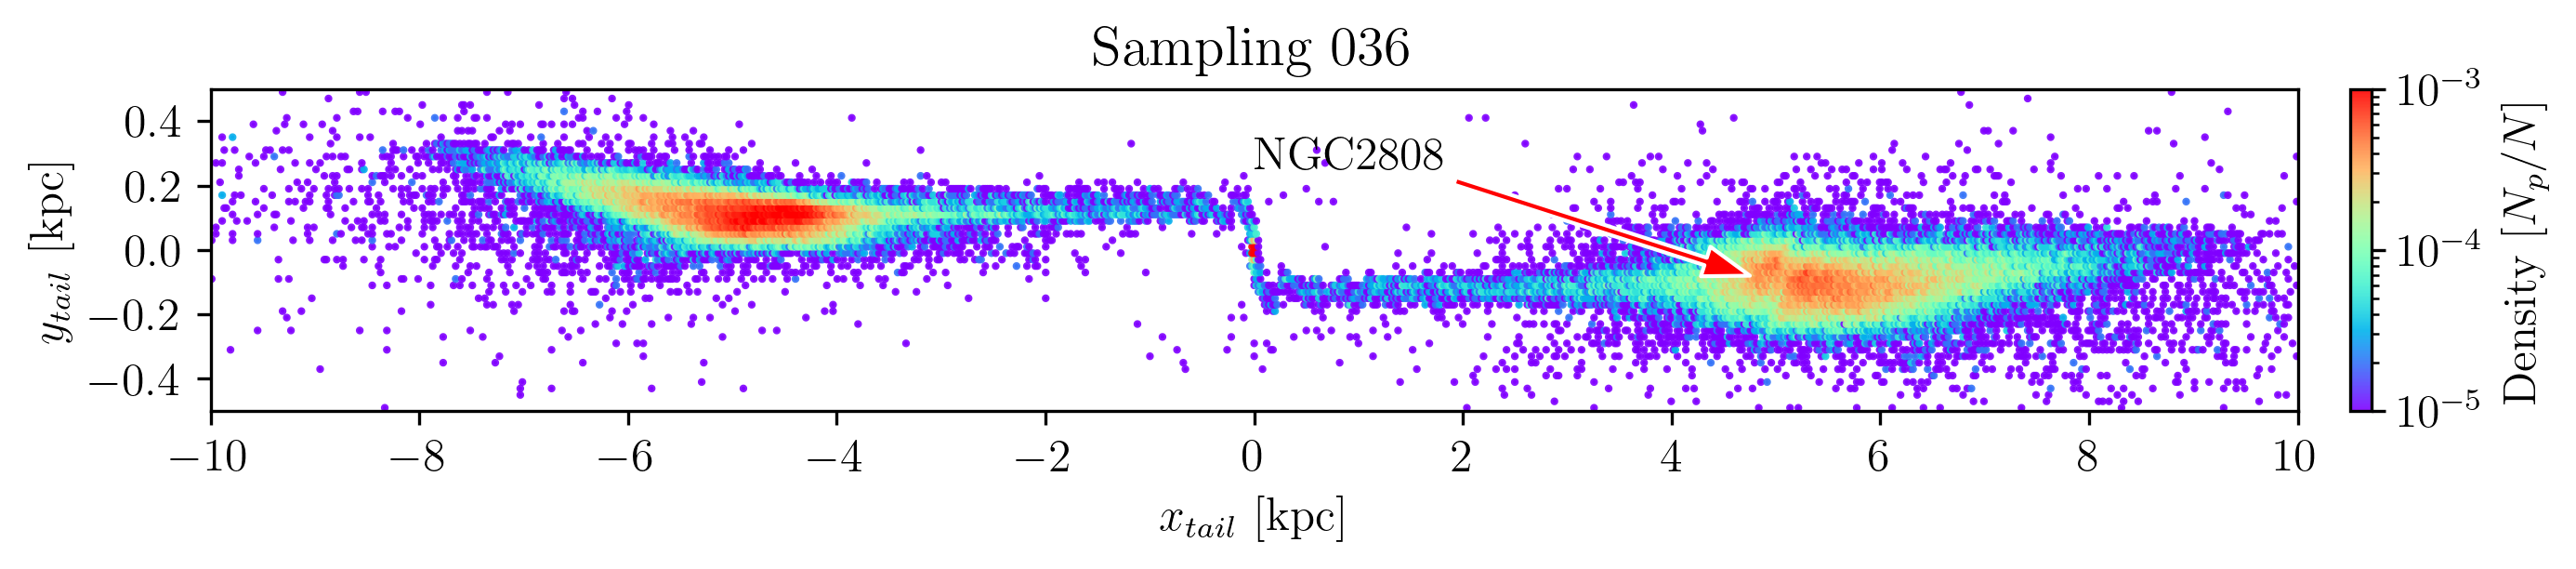
\includegraphics[width=\linewidth]{gallery_of_gaps_monte-carlo-036.png}
      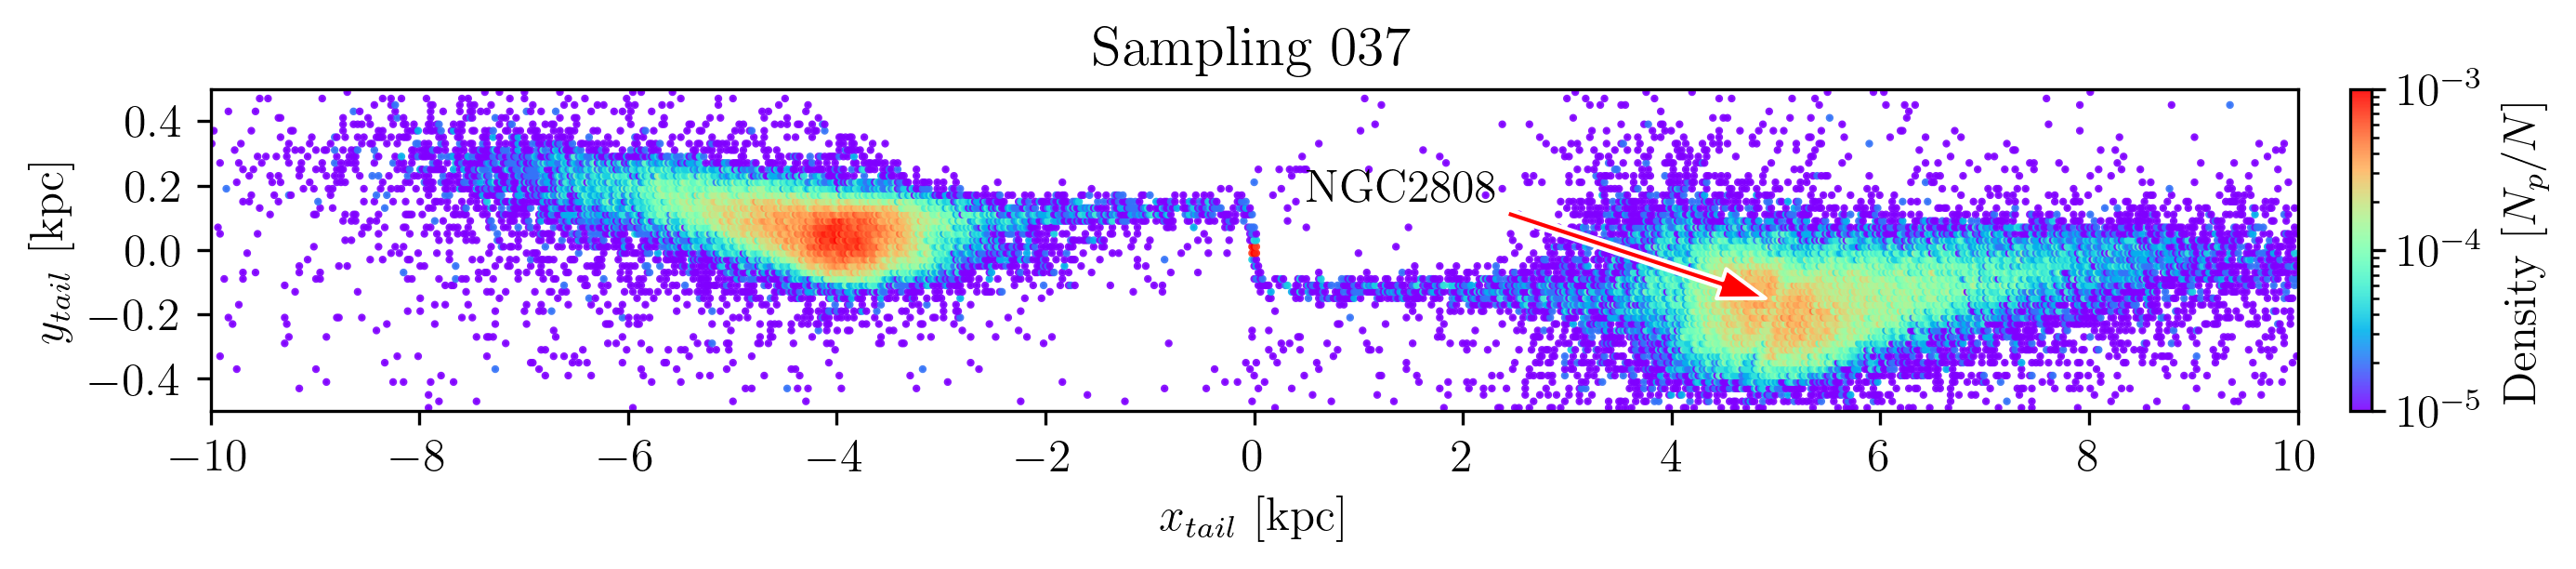
\includegraphics[width=\linewidth]{gallery_of_gaps_monte-carlo-037.png}
      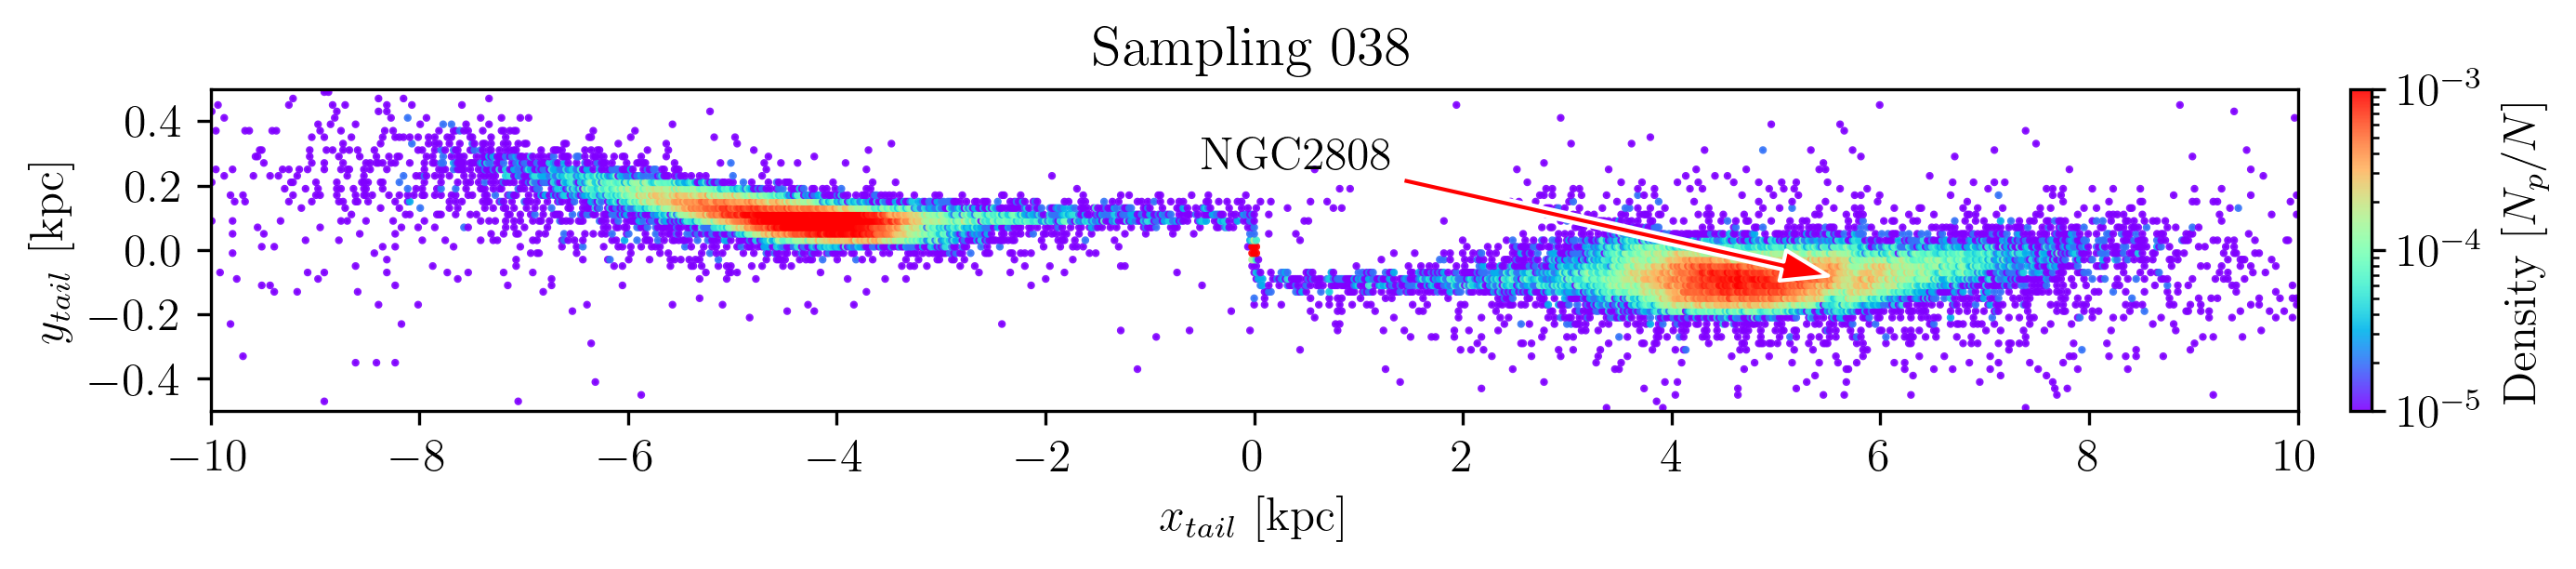
\includegraphics[width=\linewidth]{gallery_of_gaps_monte-carlo-038.png}
      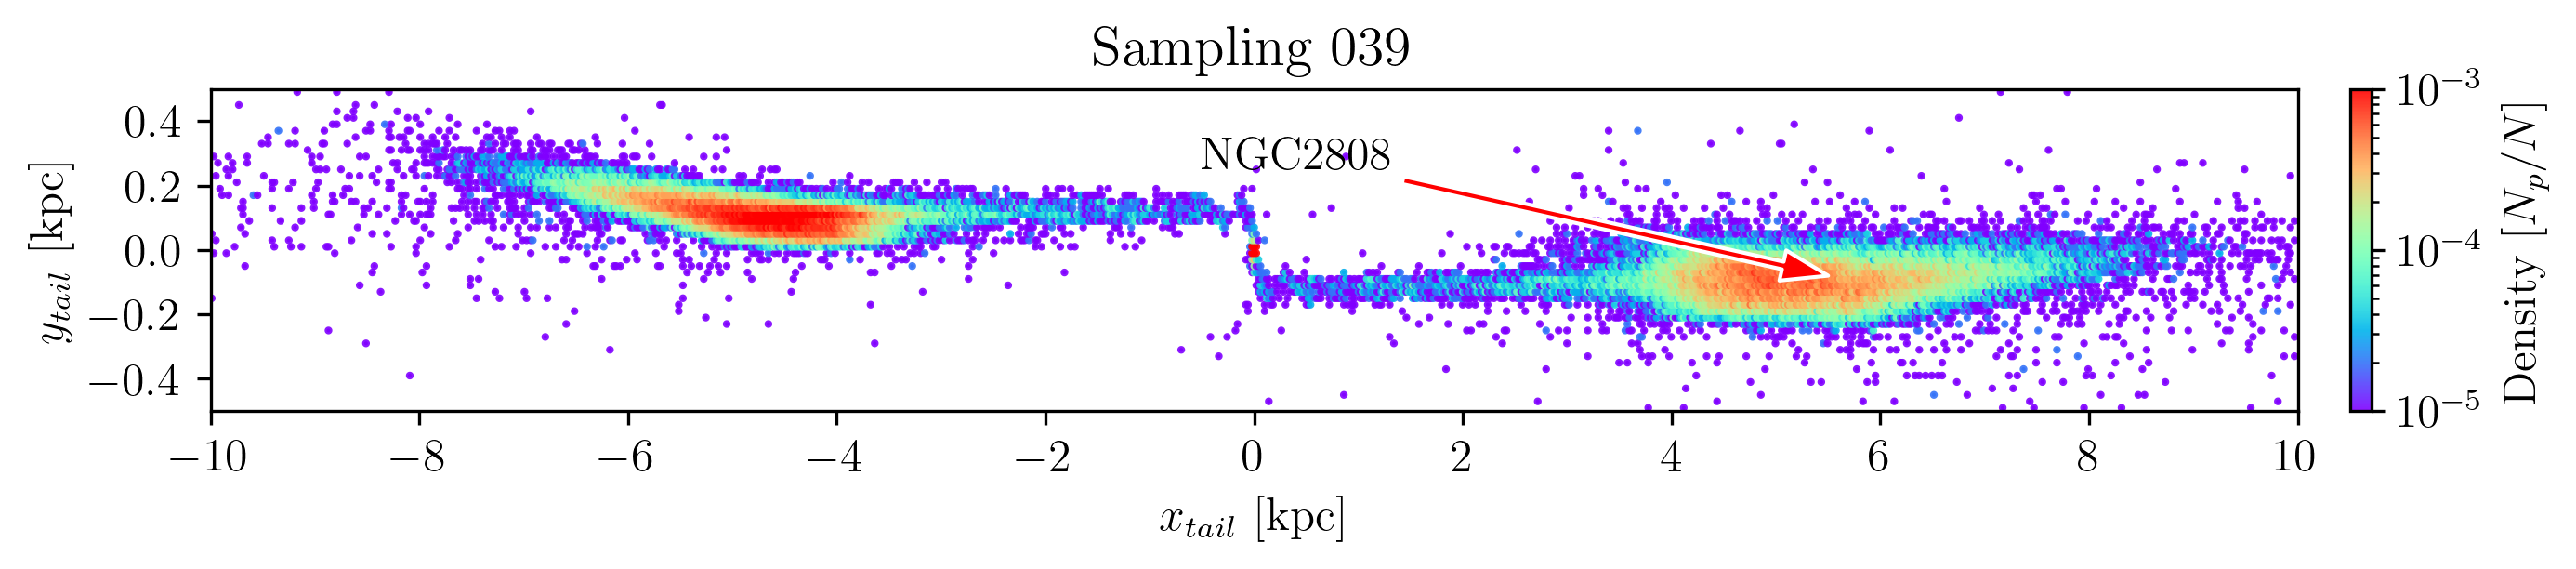
\includegraphics[width=\linewidth]{gallery_of_gaps_monte-carlo-039.png}
      \caption{Gap Gallery}
      \label{fig:TailCoordinates}
    \end{figure*}    



    \begin{figure*}
      \centering
      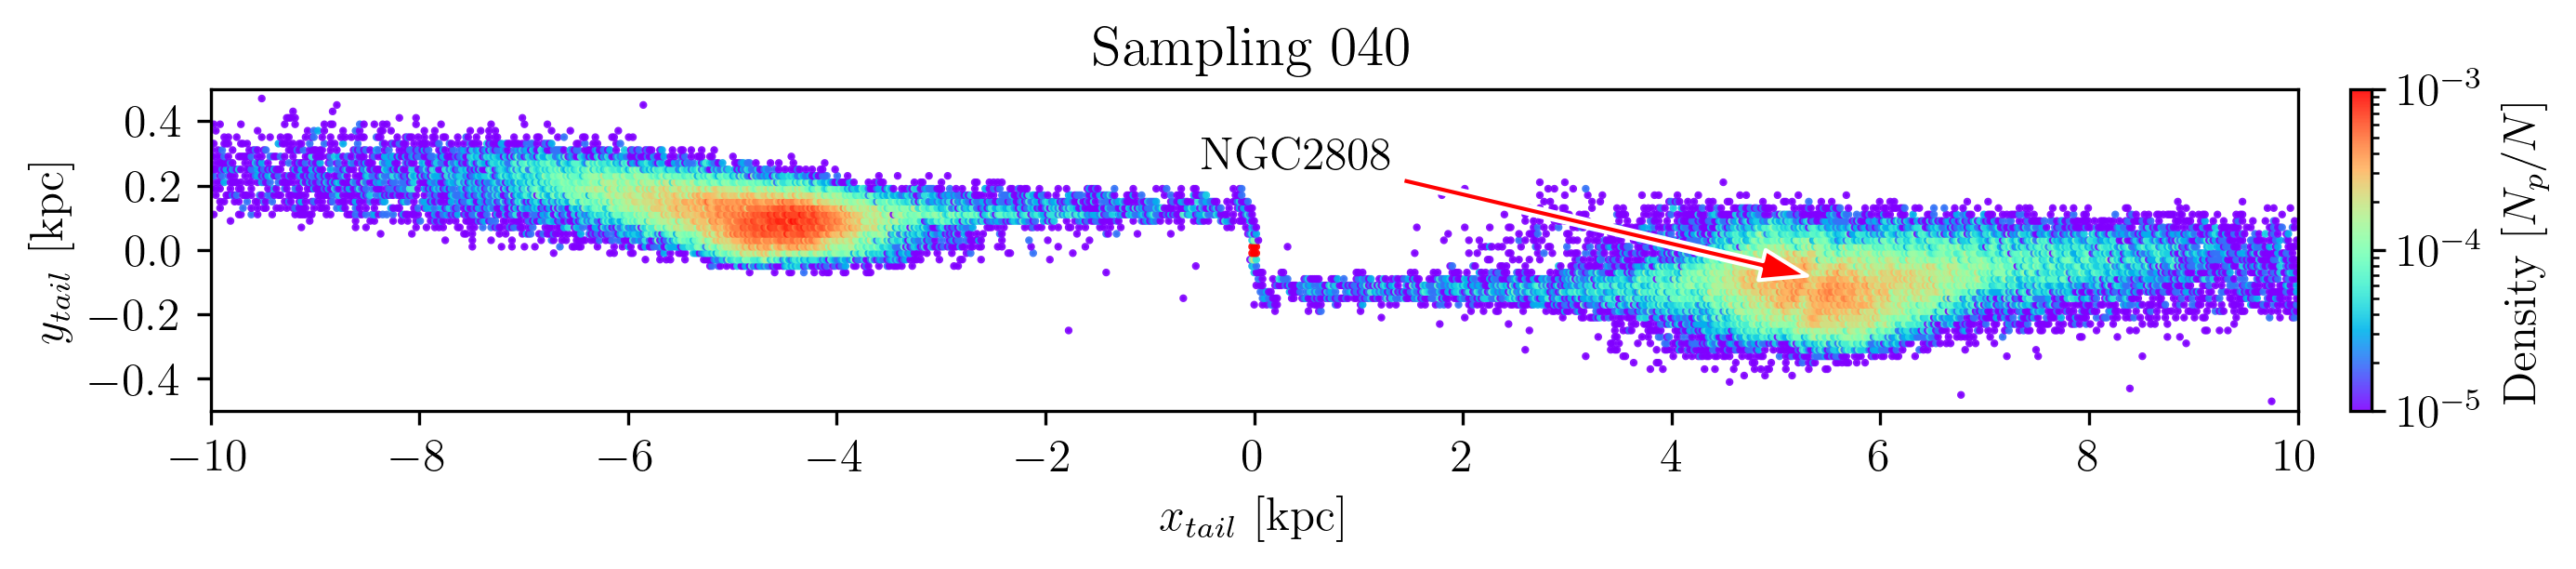
\includegraphics[width=\linewidth]{gallery_of_gaps_monte-carlo-040.png}
      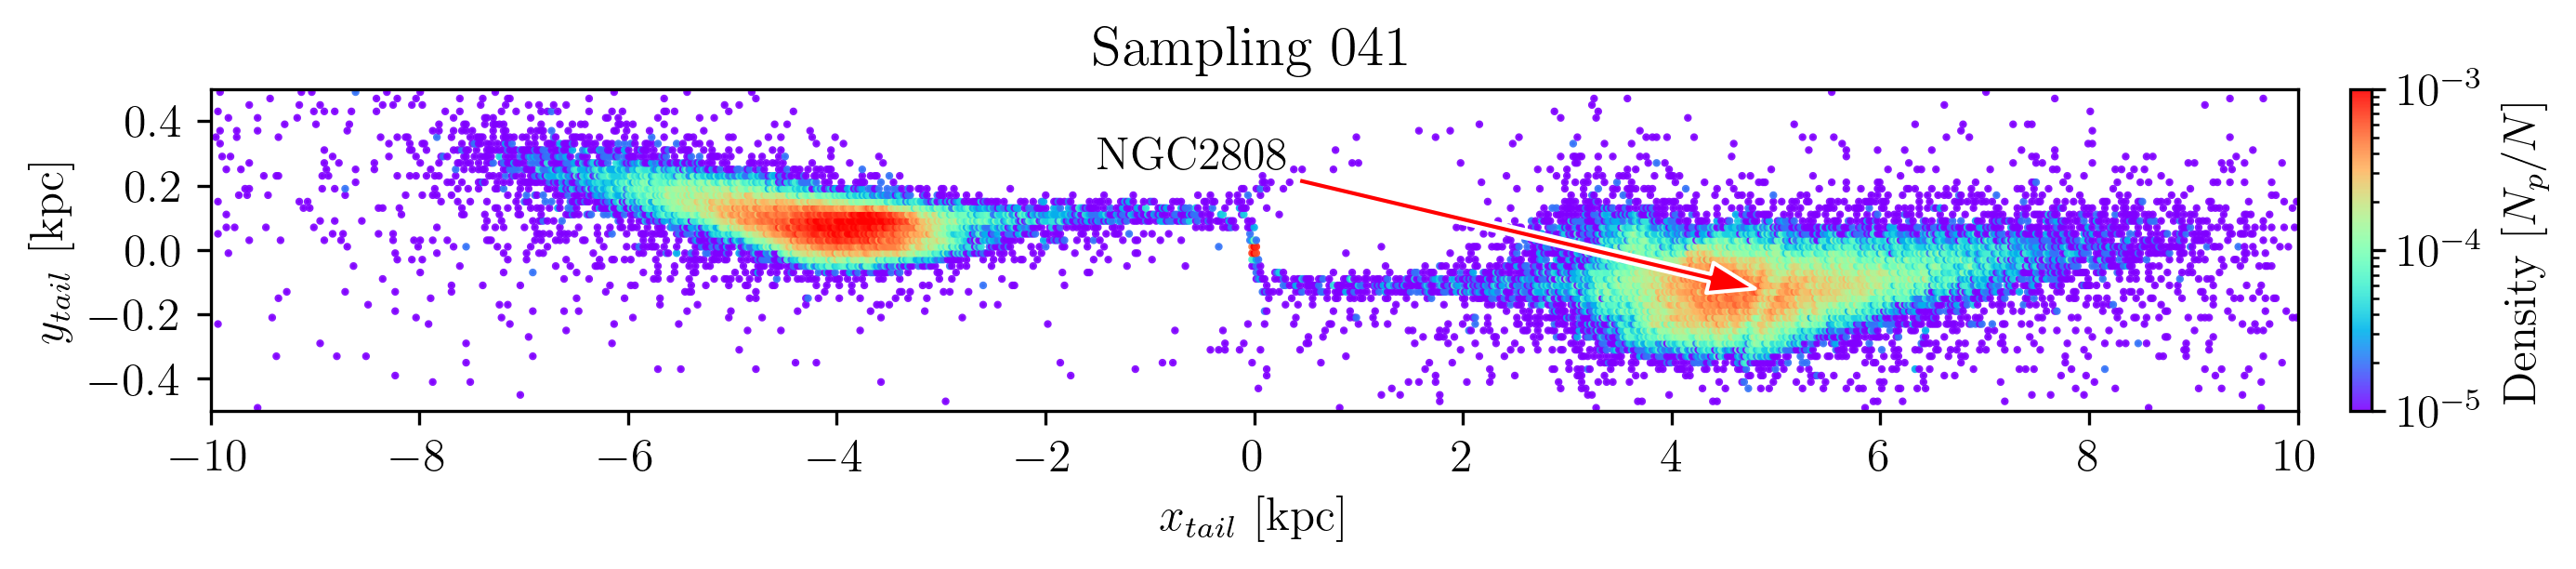
\includegraphics[width=\linewidth]{gallery_of_gaps_monte-carlo-041.png}
      \includegraphics[width=\linewidth]{gallery_of_gaps_monte-carlo-042.png}
      \includegraphics[width=\linewidth]{gallery_of_gaps_monte-carlo-043.png}
      \includegraphics[width=\linewidth]{gallery_of_gaps_monte-carlo-044.png}
      \caption{Gap Gallery}
      \label{fig:TailCoordinates}
    \end{figure*}        

    \begin{figure*}
      \centering
      \includegraphics[width=\linewidth]{gallery_of_gaps_monte-carlo-045.png}
      \includegraphics[width=\linewidth]{gallery_of_gaps_monte-carlo-046.png}
      \includegraphics[width=\linewidth]{gallery_of_gaps_monte-carlo-047.png}
      \includegraphics[width=\linewidth]{gallery_of_gaps_monte-carlo-048.png}
      \includegraphics[width=\linewidth]{gallery_of_gaps_monte-carlo-049.png}
      \caption{Gap Gallery}
      \label{fig:TailCoordinates}
    \end{figure*} 

\end{appendix}



\end{document}